% ---- ETD Document Class and Useful Packages ---- %
% This LaTeX template for Ph.D. dissertations at the University of Hanyang University.
% This template is adapted from the LaTeX template for the University of Chicago doctoral thesis:https://github.com/k4rtik/uchicago-dissertation
% Authors: Yu Zhao
\documentclass[a4paper,12pt]{HYU}
\usepackage{geometry}
\usepackage{CJKutf8}
\usepackage{algorithmic}
\usepackage{algorithm}
\setcounter{secnumdepth}{5}
\setcounter{tocdepth}{1}
\usepackage{kotex}
\usepackage{mathptmx}
\usepackage{xspace}
\usepackage{soul}
\usepackage{romannum}
\usepackage{bm}
\def\mathbi#1{\textbf{\em #1}}
\def\mathbi#1{\bm{#1}}
\usepackage{multirow}
\usepackage{pifont}% http://ctan.org/pkg/pifont
\newcommand{\cmark}{\ding{51}}%
\newcommand{\xmark}{\ding{55}}%
\usepackage{rotating}
\makeatletter
\renewenvironment{abstract}{%
    \if@twocolumn
      \section*{\abstractname}%
    \else %% <- here I've removed \small
      \begin{center}%
        {\bfseries \Large\abstractname\vspace{\z@}}%  %% <- here I've added \Large
      \end{center}%
      \quotation
    \fi}
    {\if@twocolumn\else\endquotation\fi}
\makeatother

\usepackage[utf8]{inputenc}
\setlength{\parindent}{2em}
\usepackage[T1]{fontenc}
\usepackage{indentfirst} 
\usepackage{subcaption,graphicx}
\usepackage{mathtools}  % loads amsmath
\usepackage{amssymb}    % loads amsfonts
\usepackage{amsthm}
\usepackage{nomencl}
\usepackage{array}
\DeclareMathOperator*{\argmax}{arg\,max}
\DeclareMathOperator*{\argmin}{arg\,min}
%For the abbreviations page
\newboolean{Figure}
\setboolean{Figure}{false}
\newtheorem{lemma}{Lemma}
\newtheorem{remark}{Remark}
\newtheorem{definition}{Definition}
\newtheorem{proposition}{Proposition}
\newtheorem{theorem}{Theorem}
\newtheorem{assumption}{Assumption}
\usepackage{tikz}
\newcommand*{\circled}[1]{\lower.7ex\hbox{\tikz\draw (0pt, 0pt)%
    circle (.5em) node {\makebox[1em][c]{\small #1}};}}
%% Use these commands to set biographic information for the title page:
\newcommand{\thesistitle}{Dissertation Title}
\newcommand{\thesisauthor}{Dissertation Author}
\department{Computer Science and Engineering}
\division{Dissertation Division}
\degree{Doctor of Philosophy}
\date{August 2025}
\youradvisor{Jongwon Yoon}

\definecolor{pt_stage}{HTML}{FFF47A}
\definecolor{at_stage}{HTML}{AED6CE}

\title{Towards Realistic Dense Video Captioning: Gradual, Parallel, and Adversarial Pathways}
\author{Wangyu Choi}

%% Use these commands to set a dedication and epigraph text
\dedication{Dedication Text}
\epigraph{Epigraph Text}

\usepackage{doi}
\usepackage{xurl}
\hypersetup{bookmarksnumbered,
            unicode,
            linktoc=all,
            pdftitle={\thesistitle},
            pdfauthor={\thesisauthor},
            pdfsubject={},                                % Add subject/description
            % pdfkeywords={keyword1, keyword2, keyword3}, % Uncomment and revise keywords
            pdfborder={0 0 0}}
% See https://github.com/k4rtik/ucetd-latex/issues/1
\makeatletter
\let\ORG@hyper@linkstart\hyper@linkstart
\protected\def\hyper@linkstart#1#2{%
  \lowercase{\ORG@hyper@linkstart{#1}{#2}}}
\makeatother

\begin{document}
%% Basic setup commands
% If you don't want a title page comment out the next line and uncomment the line after it:
\maketitle
%\omittitle
%\geometry{left=3.5cm,right=3.5cm,top=4cm,bottom=4cm}
% These lines can be commented out to disable the copyright/dedication/epigraph pages
% \makecopyright
% \makededication
% \makeepigraph


%% Make the various tables of contents
\newgeometry{left=3.5cm, right=3.5cm, top=4cm, bottom=4cm} 
\tableofcontents
\listoffigures
\listoftables
%\newpage
\abbreviations
\makenomenclature
\renewcommand{\nomname}{List of Abbreviations}
\printnomenclature
\hfill % add blank space




\newpage
\begin{abstract}
\begin{center}
\textbf{\fontsize{13pt}{13} \selectfont  Towards Realistic Dense Video Captioning: Gradual, Parallel, and Adversarial Pathways}
\end{center}
\addcontentsline{toc}{chapter}{Abstract}
\end{abstract}

\begin{flushleft}
\hspace{6.4cm} {\fontsize{11pt}{16} \selectfont Wangyu Choi}\\
\hspace{6.4cm} {\fontsize{11pt}{16} \selectfont Dept. of Computer Science and Engineering} \\
\hspace{6.4cm} {\fontsize{11pt}{16} \selectfont The Graduate School}\\
\hspace{6.4cm} {\fontsize{11pt}{16} \selectfont Hanyang University}
\end{flushleft}


\mainmatter
% Main body of text follows
% !TEX root = main.ex

\chapter{Introduction}
\label{chap:introduction}

\section{Background and Motivation}


The rapid advancement of artificial intelligence technology has brought revolutionary innovations to natural language processing (NLP) and computer vision, with transformative breakthroughs such as large language models \cite{Brown2020-gx,Devlin2019-ld}, attention mechanisms \cite{Vaswani2017-sc}, and vision transformers \cite{Dosovitskiy2021-vn}.
However, the multimodal domain that simultaneously processes and describes video and text content remains fraught with significant challenges \cite{rahate2021multimodal,baltrusaitis2019multimodal}.
The fundamental difficulty lies in effectively bridging the semantic gap between visual and linguistic modalities, requiring sophisticated alignment mechanisms to establish meaningful correspondences between temporal visual patterns and natural language descriptions.

Traditional video understanding technologies have predominantly focused on short, trimmed video clips, developing robust methodologies for action recognition \cite{Carreira2017-fg,Feichtenhofer2019-mh} and video classification \cite{Karpathy2014-xm}.
However, real-world applications increasingly demand the ability to capture and describe diverse events occurring within long, untrimmed videos \cite{Heilbron2015-ha}.
This paradigm shift presents substantial computational and methodological challenges, as models must process extended temporal sequences while maintaining fine-grained understanding of event boundaries and content relationships.
The transition from trimmed to untrimmed video analysis represents a fundamental evolution in video understanding, requiring novel approaches to handle the increased complexity and variability inherent in naturalistic video content.

Dense Video Captioning (DVC) has emerged as a critical technology that temporally localizes multiple events within long videos and generates accurate natural language descriptions for each identified event \cite{Krishna2017-pw}.
This technology addresses growing practical demands across diverse application domains, including automated video surveillance systems for security monitoring \cite{stallings2019automated}, intelligent sports commentary generation for broadcasting \cite{chen2024integrated}, and content-based video retrieval for large-scale media libraries \cite{luo2020comprehensive}.
The increasing volume of video content across digital platforms necessitates automated tools that can efficiently index, search, and summarize video materials, making DVC an essential component of modern multimedia systems.

In real-world video scenarios, events exhibit complex overlapping patterns and are subject to subjective interpretations that vary based on context and observer perspective \cite{long2021temporal}.
Traditional deterministic approaches, which assume a single correct interpretation for each video segment, fail to capture the inherent ambiguity and multiplicity of valid event descriptions that characterize naturalistic video content \cite{Summers2021-mz}.
This limitation becomes particularly pronounced when dealing with concurrent events, where multiple activities may occur simultaneously within the same temporal window, or when event boundaries are temporally ambiguous. 
The recognition that video interpretation involves fundamental nondeterministic elements has motivated the development of more flexible approaches that can accommodate multiple valid interpretations while maintaining coherent and contextually appropriate descriptions.

\subsection{Problem Definition and Scope}

Existing DVC models predominantly employ a sequential pipeline that performs event localization and event captioning as separate, consecutive tasks \cite{Krishna2017-pw, Li2018-ll, Wang2018-ap}.
This sequential approach inherently suffers from error propagation, where inaccuracies in the localization stage cascade to the captioning module, significantly degrading the overall quality of generated descriptions.
The localize-then-describe paradigm creates an information bottleneck that prevents the captioning module from accessing rich visual context that could inform both temporal boundary detection and language generation simultaneously.

Real-world videos present additional complexities that challenge conventional deterministic approaches to dense video captioning.
Events in untrimmed videos frequently overlap temporally, exhibit complex interdependencies, and involve subjective interpretations that vary across annotators \cite{Qasim2025-mp}.
The inherent nondeterminism in event definition and boundary delineation means that multiple valid interpretations may exist for the same video content, yet most existing methods assume a single ground truth \cite{Duan2018-qf, Shen2017-gx}. This subjectivity in event perception introduces semantic ambiguity during training, as different annotators may identify distinct event boundaries and generate diverse caption sets for identical video segments.

The computational and annotation costs associated with fully supervised dense video captioning have motivated increased interest in weakly supervised learning and large-scale pretraining approaches. While weakly supervised methods aim to reduce dependency on temporal annotations by learning from video-level captions alone \cite{Duan2018-qf, Shen2017-gx}, and pretraining approaches leverage large-scale video-text datasets to improve model generalization \cite{Yang2023-fm, Huang2020-as}, these methodologies remain underexplored in their practical application to real-world scenarios. The challenge lies in effectively bridging the gap between weak supervision signals and the precise temporal localization required for dense captioning, while maintaining caption quality and coherence.

Consequently, there is a critical need for methodological innovations that address four key limitations: efficient detection of overlapping and temporally complex events, minimization of information loss through parallel processing architectures, improved learning efficiency through weakly supervised and pretraining strategies, and realistic captioning approaches that accommodate the inherent nondeterminism in event interpretation. These challenges motivate the development of diverse algorithmic strategies that can handle the multifaceted nature of dense video captioning while maintaining practical applicability in real-world scenarios.



\subsection{Research Objectives}

To address the aforementioned challenges in dense video captioning, this research aims to develop and evaluate four distinct yet complementary approaches that tackle different aspects of the fundamental limitations in existing methods. Each approach represents a targeted solution to specific problems while contributing to the overall advancement of dense video captioning technology.

First, we propose a gradual Step-by-Step (SBS) framework that explicitly predicts the number of events in a video and progressively detects event boundaries based on this prediction. Unlike conventional approaches that rely on fixed proposal generation schemes \cite{Krishna2017-pw, Wang2018-ap}, our method addresses the challenge of overlapping and variable-length events by implementing a human-inspired progressive detection strategy. This approach aims to improve the precision of event localization, particularly in scenarios where events exhibit complex temporal overlaps and varying durations \cite{Choi2023-so}.

Second, we introduce a Parallel Pathway Dense Video Captioning (PPVC) framework that breaks away from the traditional sequential ``localize-then-describe'' pipeline.
While existing methods suffer from error propagation between event detection and caption generation stages \cite{Zhou2018-zu, Mun2019-ap}, our parallel approach performs event localization and captioning simultaneously without bottlenecks. 
By incorporating deformable transformers \cite{Vaswani2017-sc} and multi-stack cross-attention mechanisms, this framework minimizes information loss and reduces the dependency on the performance of preceding modules \cite{Choi2022-cu}.

Third, we develop a Pretraining-based Weakly Supervised Dense Video Captioning (PWS-DVC) approach that leverages large-scale clip-level caption datasets for model initialization without requiring explicit event-level annotations.
This method addresses the annotation scarcity problem inherent in dense video captioning \cite{Shen2017-gx, Duan2018-qf} by utilizing readily available video-caption pairs from datasets such as WebVid and YT-Temporal-1B.
The pretraining strategy enhances model generalization and learning stability in weakly supervised scenarios while maintaining competitive performance compared to fully supervised methods.

Fourth, we propose an Adversarial Dense Video Captioning (ADVC) framework that explicitly models the nondeterministic nature of event interpretation and caption generation.
Recognizing that dense video captioning inherently involves subjective judgments and multiple valid interpretations \cite{Goodfellow2014-hs}, this approach employs adversarial training to generate diverse and realistic event descriptions.
The framework consists of unsupervised pretraining on large-scale unlabeled data followed by adversarial adaptation, enabling the model to capture the distribution of human-annotated events and produce varied yet coherent captions for the same video content.

Each of these approaches targets specific limitations in current dense video captioning systems: the SBS framework addresses event detection precision, PPVC eliminates pipeline bottlenecks, PWS-DVC tackles annotation requirements, and ADVC handles interpretation diversity.
Through comprehensive experimental evaluation on standard benchmarks including ActivityNet Captions \cite{Krishna2017-pw} and YouCook2 \cite{Zhou2018-eq}, we aim to demonstrate that these methods not only advance the state-of-the-art in their respective problem domains but also provide complementary solutions that can be integrated for more robust and practical dense video captioning systems.

The ultimate objective of this research is to contribute to the development of more accurate, efficient, and realistic dense video captioning models that can handle the complexity and diversity of real-world video content, thereby enabling broader applications in video understanding, content retrieval, and multimedia accessibility.


\subsection{Contributions}
This dissertation addresses the primary limitations of dense video captioning by clearly defining key challenges and proposing four novel approaches (SBS, PPVC, PWS-DVC, and ADVC) to overcome them, with experimental validation demonstrating the effectiveness and synergistic integration of each approach.
Unlike existing methods that typically focus on a single aspect of the problem \cite{Krishna2017-pw, Zhou2018-zu, Mun2019-ap}, our comprehensive framework systematically tackles multiple fundamental issues including sequential pipeline limitations, data scarcity, and the nondeterministic nature of event interpretation.
The proposed unified framework advances the state-of-the-art by addressing both methodological and practical challenges that have hindered the deployment of dense video captioning systems in real-world applications.

We propose the Step-by-Step (SBS) approach that explicitly predicts the number of events and progressively processes overlapping events, and the Parallel Pathway with Deformable Transformer (PPVC) approach that simultaneously performs event detection and captioning to eliminate the bottleneck effects inherent in sequential pipelines.
The SBS framework addresses the challenge of overlapping and nested events by introducing a gradual refinement mechanism that iteratively improves event boundary detection \cite{Chen2021-sv, Deng2021-qd}.
Meanwhile, PPVC overcomes the error propagation problem common in traditional ``localize-then-describe'' pipelines \cite{Li2018-ll, Wang2018-ap} by employing parallel decoding strategies with deformable attention mechanisms, thereby reducing information loss and improving overall captioning consistency \cite{Choi2022-cu}.

To address the data scarcity problem, we introduce the Pretraining-based Weakly Supervised Dense Video Captioning (PWS-DVC) framework that leverages large-scale clip-level caption datasets for effective pretraining without requiring event-level annotations, and the Adversarial Dense Video Captioning (ADVC) approach that models the nondeterministic nature of event definitions through adversarial learning to achieve realistic captioning performance.
The PWS-DVC framework demonstrates that effective dense video captioning models can be trained using readily available video-caption pairs without expensive temporal localization annotations \cite{Huang2020-as, Luo2022-yq}, while ADVC addresses the fundamental challenge that multiple valid interpretations exist for the same video content \cite{Seo2022-ok, Yang2023-fm}.
These approaches significantly improve the practical applicability of dense video captioning by reducing annotation requirements and handling the inherent ambiguity in video interpretation.

Through comprehensive evaluation on standard benchmarks including ActivityNet Captions and YouCook2, we demonstrate that our integrated framework achieves superior performance compared to existing state-of-the-art methods across both quantitative metrics (METEOR, CIDEr, BLEU) and qualitative assessments.
Our experimental validation includes extensive ablation studies that verify the individual contribution of each proposed component, cross-dataset generalization experiments that demonstrate robustness across different domains, and comprehensive analysis of computational efficiency compared to baseline methods \cite{Krishna2017-pw, Zhou2018-zu, Wang2021-zi}.
The results consistently show significant improvements in captioning quality, temporal localization accuracy, and system robustness, establishing new benchmarks for dense video captioning performance while maintaining practical computational requirements for real-world deployment.


\subsection{Dissertation Organization}
\label{sec:dissertation_organization}

This dissertation is structured around four distinct approaches to address various challenges in dense video captioning, with each chapter systematically presenting the design motivation, model architecture, experimental evaluation, and analysis of the respective approach.

\textbf{Chapter~\ref{chap:related_work}} provides a comprehensive overview of the research background and development trends in dense video captioning. We categorize existing research according to their methodological approaches (e.g., sequential, parallel, weakly supervised, and generative) and establish the positioning and distinctive contributions of the four approaches proposed in this dissertation.

\textbf{Chapter~\ref{chap:gradual_pathway}} introduces the Step-by-Step (SBS) framework, a gradual detection-based approach that explicitly predicts the number of events and progressively localizes event boundaries based on this estimation. We demonstrate how this method enhances the precision of overlapping event detection through sequential captioning strategies.

\textbf{Chapter~\ref{chap:parallel_pathway}} presents the Parallel Pathway with Deformable Transformer (PPVC) architecture, which performs event detection and sentence generation in parallel to overcome the bottleneck and error propagation issues inherent in traditional sequential (localize-then-describe) pipelines.
We detail the bottleneck-free branching design and improvements achieved through multi-stack cross-attention mechanisms.

\textbf{Chapter~\ref{chap:pws_dvc}} introduces the Pretraining-based Weakly Supervised Dense Video Captioning (PWS-DVC) framework.
This approach demonstrates how large-scale clip-level caption datasets can be effectively utilized for model training without event-level annotations, and evaluates the generalization performance of this stable learning framework under weakly supervised conditions.

\textbf{Chapter~\ref{chap:adversarial_pathway}} describes the Adversarial Dense Video Captioning (ADVC) framework, which incorporates nondeterminism through adversarial generative learning.
This approach accommodates multiple possible interpretations in realistic video scenarios and experimentally validates the diversity and consistency of generated captions that embrace various expression possibilities.

\textbf{Chapter~\ref{chap:conclusions}} summarizes the overall contributions of this dissertation, discusses the limitations of each approach and improvement directions for practical applications, and presents future research challenges in the field of dense video captioning.

Each approach addresses independent problem formulations and solution strategies, and this dissertation systematically evaluates the methodological validity and practical effectiveness of each through comprehensive quantitative and qualitative metrics.
% !TEX root = ./main.tex

\chapter{Related Work}
\label{chap:related_work}

%------------------------------------------------------------------------------
\section{Related Work}
%------------------------------------------------------------------------------

Dense–video–captioning (DVC) research builds on three lines of prior work:  
(i) sentence–level \emph{video clip captioning},  
(ii) \emph{dense} captioning of untrimmed videos under various supervision and architectural regimes, and  
(iii) emerging techniques that exploit large–scale pre-training or adversarial learning to mitigate data sparsity and subjectivity.  
We synthesise the literature along these axes, following the analytical structure suggested by our thesis ToC.

%------------------------------------------------------------------------------
\subsection{Video Clip Captioning}
%------------------------------------------------------------------------------
Early studies generate a single sentence per \emph{trimmed} video via an encoder–decoder paradigm that mirrors neural machine translation \cite{sutskever2014sequence,cho-etal-2014-learning}.  
CNNs encode frame sequences while RNNs (LSTM/GRU) \cite{venugopalan2015sequence,venugopalan2015translating} decode word tokens.  
Enhancements include temporal attention \cite{yao2015describing}, hierarchical decoders \cite{pan2016hierarchical,baraldi2017hierarchical}, multimodal/semantic embeddings \cite{pan2016jointly,gan2017semantic,pan2017video,yu2017end}, spatial–hard attention \cite{liu2018fine}, reconstruction losses \cite{wang2018reconstruction}, and reinforcement learning for adaptive attention \cite{xiao2019video}.  
Although paragraph-level extensions exist \cite{yu2016video,xiong2018move,lei2020mart}, clip-level methods cannot describe long, overlapping events and therefore motivate DVC.

%------------------------------------------------------------------------------
\subsection{Dense Video Captioning}
%------------------------------------------------------------------------------
\subsubsection{Sequential Bottom-Up / Top-Down Paradigms}  
The seminal bottom-up DEC detects temporal proposals with LSTMs and captions them sequentially \cite{Krishna2017-pw}.  
Follow-ups improve localisation via descriptiveness prediction \cite{Li2018-ll}, bidirectional context \cite{Wang2018-ap}, or single-stream proposals \cite{Mun2019-ap}.  
Top-down pipelines invert the order: paragraph generation precedes sentence-to-segment grounding \cite{Deng2021-qd}.  
Both suffer from error propagation and often rely on NMS or threshold heuristics, which hampers overlapping–event recall \cite{lin2018bsn}.

\subsubsection{Parallel and End-to-End Transformers}  
Masked-transformer DVC \cite{Zhou2018-zu} and deformable-transformer PDVC \cite{Wang2021-zi} remove explicit proposal networks and decode localisation \emph{and} language jointly, leveraging self-attention’s long-range modelling superiority over LSTMs \cite{vaswani2017attention}.  
PPVC further alleviates branch bottlenecks through a representation organiser, gating network, and multi-stack cross attention, boosting performance on ActivityNet and YouCook2 \cite{Choi2023-so}.

\subsubsection{Pre-training for Data Efficiency}  
Limited manual annotations inspire vision–language pre-training.  
E2ESG transfers the WikiHow-pre-trained T5 captioner into DVC \cite{Zhu2022-mg}.  
UEDVC self-pre-trains on ActivityNet captions \cite{Zhang2022-ni}, whereas Vid2Seq scales to narrated YouTube videos with ASR transcripts \cite{Yang2023-fm}.  
These sequence-to-sequence models excel at lexical diversity but still depend on noisy narration and couple localisation tightly to generation.

\subsubsection{Weakly Supervised DVC}  
WS-DEC \cite{Duan2018-qf} and EC-SL \cite{Chen2021-sv} replace proposal detection with alternating \emph{event captioning} and \emph{caption localisation}, requiring only sentence supervision.  
PWS-DVC enhances this regime by pre-training the captioner on MSR-VTT and fine-tuning jointly, closing much of the gap to fully-supervised systems \cite{Aafaq2023-vk}.

\subsubsection{Gradual Reasoning for Overlapping Events}  
SBS adopts a human-like \emph{step-by-step} strategy: explicit event counting (Temporal Event Counter), boundary classification, and context-aware sentence generation.  
This avoids hand-crafted NMS, achieves high recall on overlapping regions, and remains interpretable \cite{StepByStep2023}.

%------------------------------------------------------------------------------
\subsection{Design Considerations Across Paradigms}
%------------------------------------------------------------------------------
\paragraph{Temporal Encoding.}  
Transformers capture long-term dependencies in untrimmed videos and allow parallel training, whereas LSTMs are sequential but memory-efficient \cite{krishna2017dense,zhou2018end,wang2021end}.  

\paragraph{End-to-End vs.\ Modular Training.}  
While end-to-end models back-propagate global losses, higher inductive-bias modular designs (e.g., TEC+TBC in SBS) can excel when training data are scarce.

\paragraph{Event Representation.}  
Heat-map generators and deformable sets bypass proposal filtering; query-based systems must balance query count with precision–recall trade-offs \cite{Choi2023-so}.

%------------------------------------------------------------------------------
\subsection{Adversarial and Object-Centric Extensions}
%------------------------------------------------------------------------------
Adversarial DVC (ADVC) frames localisation–captioning as a generative task: a video-conditioned GAN learns the distribution of human event sets, while a sentence GAN bridges video and language embeddings for realistic, diverse captions \cite{ssrn-4835759}.  
Object-oriented variants incorporate structured trajectories and GAN critics to capture fine-grained entity interactions, improving descriptiveness in complex scenes \cite{Zhu2022-mg}.

%------------------------------------------------------------------------------
\subsection{Summary}
%------------------------------------------------------------------------------
Research has progressed from sequential LSTM frameworks to transformer-based, parallel, pre-trained, weakly supervised, and adversarial models.  
Gradual reasoning improves overlapping-event recall; parallel deformable transformers alleviate bottlenecks; large-scale pre-training broadens linguistic coverage; and adversarial learning tackles subjectivity.  
Our work unifies these complementary advances to push dense video captioning towards detailed, coherent, and human-like descriptions of long, real-world videos.

% !TeX root = main.tex

\chapter{Gradual Approach: Step by Step Framework}
\label{chap:gradual_pathway}

\section{Human-inspired Video Understanding}
\label{sec:human_inspired}

\begin{sidewaysfigure}
  \centering
  \includegraphics[width=1\columnwidth]{figures/sbs_intro_overview.pdf}
  \caption{
    Comparison between the existing methods and ours for dense video captioning.
    Similar to human interpretation, the proposed algorithm first scans a given video and explicitly determines the number of events.
    It then generates events by specifying the start and end timestamps of the salient region based on the number of events.
    Finally, it describes a specific sentence for each event region.
    On the other hand, existing methods generate a large number of event proposals and then remove duplicates with a han-crafted algorithm such as NMS.\@
    This makes it difficult to detect different events (i.e., actions) in the same time period.
  }
  \label{fig:intro_overview}
\end{sidewaysfigure}

% \begin{figure}[t]
%   \centering
%   \includegraphics[width=1\textwidth]{figures/sbs_intro_overview.pdf}
%   \caption{
%     Comparison between the existing methods and ours for dense video captioning.
%     Similar to human interpretation, the proposed algorithm first scans a given video and explicitly determines the number of events.
%     It then generates events by specifying the start and end timestamps of the salient region based on the number of events.
%     Finally, it describes a specific sentence for each event region.
%     On the other hand, existing methods generate a large number of event proposals and then remove duplicates with a han-crafted algorithm such as NMS.\@
%     This makes it difficult to detect different events (i.e., actions) in the same time period.
%   }
%   \label{fig:intro_overview}
% \end{figure}

Human video understanding exhibits remarkable capabilities that current computational models struggle to replicate~\cite{Heilbron2015-ha,Krishna2017-pw}. When humans observe complex video sequences, they naturally employ a systematic cognitive process: first assessing the overall scene to estimate the number of concurrent activities, then focusing attention on specific temporal boundaries where events begin and end, and finally constructing coherent narratives that capture both individual events and their contextual relationships~\cite{wang2020event,long2021temporal}. This human-centric approach contrasts sharply with existing computational methods that rely heavily on exhaustive proposal generation followed by heuristic filtering mechanisms.

Current dense video captioning systems predominantly adopt bottom-up paradigms that generate numerous temporal proposals and subsequently eliminate redundancies using hand-crafted algorithms such as non-maximum suppression (NMS)~\cite{Krishna2017-pw,Li2018-ll,Wang2018-ap,Zhou2018-zu}. While these approaches have demonstrated effectiveness in controlled scenarios, they fundamentally diverge from human perceptual strategies and suffer from critical limitations when processing overlapping events. The reliance on temporal overlap thresholds rather than semantic content analysis leads to the inadvertent removal of distinct activities that occur within similar timeframes, thereby compromising the richness and accuracy of video descriptions~\cite{Mun2019-ap,fujita2020soda}.

The cognitive science literature suggests that human event perception involves hierarchical processing mechanisms that operate from global scene understanding to fine-grained temporal segmentation~\cite{zacks2007event,kurby2008segmentation}. Humans demonstrate superior performance in identifying event boundaries by leveraging contextual cues, semantic knowledge, and temporal dynamics simultaneously. This multi-faceted approach enables robust detection of overlapping activities and generation of coherent narratives that maintain both local accuracy and global consistency~\cite{radvansky2006event,speer2007reading}.

Motivated by these observations, we propose a human-inspired framework for dense video captioning that mirrors the natural cognitive process of video understanding. As illustrated in Figure~\ref{fig:intro_overview}, our approach implements a systematic progression from abstract scene assessment to detailed event description. Rather than generating numerous proposals indiscriminately, our method first estimates the explicit number of events present in each temporal region, providing crucial guidance for subsequent localization and captioning procedures.

Our framework operationalizes human-like video understanding through five sequential stages that reflect natural perceptual processes. Initially, the system performs global scene analysis to estimate the \textit{number of concurrent events}, departing from binary actionness classification toward explicit event counting that better captures the complexity of overlapping activities~\cite{yuan2017temporal,lin2018bsn}. Subsequently, the framework identifies \textit{event boundaries} by detecting semantic transitions and temporal discontinuities that correspond to activity onset and termination points~\cite{long2019gaussian,zhao2020bottom}. This boundary detection process enables precise temporal localization without relying on predetermined proposal sets.

The third stage synthesizes event count estimates and boundary information to generate a refined set of event proposals using an actionness-weighted temporal Intersection over Union (tIoU) algorithm, eliminating the need for conventional proposal selection mechanisms that ignore semantic content~\cite{lin2019bmn,hosang2017learning}. The fourth stage implements \textit{contextual encoding} of event proposals to ensure coherence and narrative consistency, reflecting the human tendency to construct interconnected rather than isolated event descriptions~\cite{zhu2020understanding,wang2018temporal}. Finally, the framework generates natural language descriptions through a hierarchical sentence construction process that maintains both local accuracy and global narrative coherence.

This human-inspired approach addresses fundamental limitations in existing dense video captioning systems by incorporating cognitive principles that enable robust handling of overlapping events, contextual understanding, and coherent narrative generation. The explicit modeling of human perceptual strategies provides a principled foundation for developing more effective and interpretable video understanding systems that can handle the complexity and ambiguity inherent in real-world video content~\cite{bhooshan2022multimodal,li2022adaptive}.



\section{Step-by-Step (SBS) Framework}

%In this section, we describe the core idea of SBS, dense video captioning framework.
\subsection{Overview} 
\label{subsec:method_overview}

\begin{sidewaysfigure}
  \centering
  \includegraphics{figures/sbs_design_overview.pdf}
  \caption{
    Overview of the Step-by-Step (SBS) framework for dense video captioning.
    (1) \textbf{Video encoder}: Extracts spatiotemporal features using C3D networks and encodes long-range temporal dependencies via transformer encoder.
    (2) \textbf{Temporal event counter}: Explicitly estimates the number of events at each temporal location.
    (3) \textbf{Temporal boundary classifier}: Localizes event start and end boundaries along the timeline.
    (4) \textbf{Event proposal generation}: Generates event proposals from predicted counts and boundaries without relying on hand-crafted selection algorithms.
    (5) \textbf{Context-level event encoder}: Encodes sequences of event proposals to capture inter-event dependencies.
    (6) \textbf{Sequential event captioner}: Generates natural language descriptions for each localized event using context-aware features.
  }
  \label{fig:method_overview}
\end{sidewaysfigure}

% \begin{figure*}[t]
%   \centering
%   \includegraphics[width=1\textwidth]{figures/sbs_design_overview.pdf}
%   \caption{
%     Overview of the Step-by-Step (SBS) framework for dense video captioning.
%     (1) \textbf{Video encoder}: Extracts spatiotemporal features using C3D networks and encodes long-range temporal dependencies via transformer encoder.
%     (2) \textbf{Temporal event counter}: Explicitly estimates the number of events at each temporal location.
%     (3) \textbf{Temporal boundary classifier}: Localizes event start and end boundaries along the timeline.
%     (4) \textbf{Event proposal generation}: Generates event proposals from predicted counts and boundaries without relying on hand-crafted selection algorithms.
%     (5) \textbf{Context-level event encoder}: Encodes sequences of event proposals to capture inter-event dependencies.
%     (6) \textbf{Sequential event captioner}: Generates natural language descriptions for each localized event using context-aware features.
%   }
%   \label{fig:method_overview}
% \end{figure*}

The Step-by-Step (SBS) framework addresses the fundamental challenge of overlapping event detection in dense video captioning through a human-inspired progressive approach, as illustrated in Figure~\ref{fig:method_overview}. 
Unlike conventional methods that rely on proposal-based architectures with non-maximum suppression (NMS)~\cite{Krishna2017-pw,Li2018-ll}, SBS explicitly models the number of events and their temporal boundaries to achieve more precise localization of overlapping events.

The framework comprises six interconnected modules that process videos in a systematic manner.
Given an input video $V$, the \textbf{video encoder} first extracts spatiotemporal features using C3D networks~\cite{Tran2015-uq} and applies a transformer encoder~\cite{Vaswani2017-sc} to capture long-range temporal dependencies across the entire video sequence.
This encoding strategy effectively handles the temporal complexity inherent in untrimmed videos while preserving fine-grained visual information necessary for accurate event detection.

The core innovation of SBS lies in its explicit event quantification approach.
The \textbf{temporal event counter} estimates the number of overlapping events at each temporal location, providing crucial guidance for subsequent localization stages.
This differs fundamentally from binary actionness scoring used in existing methods~\cite{lin2018bsn,buch2017sst}, enabling the detection of multiple concurrent events within the same temporal region.
Subsequently, the \textbf{temporal boundary classifier} performs fine-grained localization by identifying event start and end boundaries along the timeline, leveraging the count information to guide boundary detection accuracy.

Event proposals are then generated through the \textbf{event proposal generation} module, which combines the predicted event counts and boundary classifications to produce temporally coherent event segments.
Crucially, this approach eliminates the need for hand-crafted selection algorithms such as NMS, which often suppress valid overlapping events and compromise recall performance~\cite{hosang2017learning}.

To ensure coherent and contextually appropriate caption generation, SBS employs a two-stage captioning architecture.
The \textbf{context-level event encoder}, implemented as a single-layer LSTM, processes the sequence of event proposals to capture inter-event dependencies and contextual relationships within the video narrative.
This context-aware encoding addresses the limitation that events in dense videos are not independent but form coherent temporal sequences that require understanding of their relationships.

Finally, the \textbf{sequential event captioner} generates natural language descriptions for each localized event by leveraging both the visual features of individual events and the context-encoded representations.
This sequential generation process ensures that the produced captions maintain narrative coherence and contextual appropriateness across the entire video sequence, addressing the challenge of generating fluent and coherent descriptions for multiple related events~\cite{Yu2016-il,Lei2020-tg}.

The progressive nature of the SBS framework, from explicit event counting to boundary detection and context-aware captioning, mirrors human cognitive processes in understanding complex video content.
This design choice not only improves localization accuracy for overlapping events but also enhances the interpretability of the model's decision-making process, making it more suitable for applications requiring transparent and reliable video understanding capabilities.

\subsection{Video Encoder}
\label{subsec:method_video_encoder}

The video encoder serves as the foundation of our SBS framework, responsible for extracting rich spatiotemporal representations from untrimmed videos that enable subsequent event counting and boundary classification. Given the varying lengths and complex temporal structures of untrimmed videos in dense captioning scenarios, we design a two-stage encoding architecture that combines spatial feature extraction with temporal dependency modeling.

\textbf{Video Preprocessing and Segmentation.}
For a given input video $V$, we first divide it into non-overlapping, fixed-length snippets $V=\{v_n\}_{n=1}^{T}$, where each snippet $v_n$ contains 8 consecutive frames. This snippet-based representation follows established practices in video understanding \cite{Wang2019-xv,Feichtenhofer2019-mh} and provides a manageable computational unit while preserving temporal coherence. The fixed snippet length of 8 frames balances computational efficiency with temporal granularity, as empirically validated in previous video captioning works \cite{Krishna2017-pw,Zhou2018-zu}.

The choice of non-overlapping segmentation, while potentially losing some temporal continuity, offers several advantages: (i) reduced computational complexity for long videos, (ii) clear temporal boundaries for subsequent event localization, and (iii) compatibility with standard video feature extraction pipelines \cite{Carreira2017-fg,Tran2015-uq}.

\textbf{Spatial Feature Extraction.}
Our video encoder employs a two-component architecture consisting of a CNN backbone for spatial feature extraction followed by a transformer encoder for temporal dependency modeling. This hybrid design leverages the complementary strengths of convolutional and attention-based architectures \cite{Dosovitskiy2021-vn,Arnab2021-gv}.

For spatial feature extraction, we adopt the C3D network \cite{Tran2015-uq} as our CNN backbone due to its proven effectiveness in capturing spatiotemporal patterns in video data. C3D extends traditional 2D convolutions to 3D, enabling simultaneous processing of spatial and short-term temporal information within video clips \cite{Karpathy2014-xm}. The network takes each snippet $v_n$ as input and produces feature representations $\mathbf{f}_n \in \mathbb{R}^{d_f}$, where $d_f$ denotes the feature dimension.

The complete spatial feature extraction process yields:
\begin{equation}
  \mathbf{F}_v = \text{C3D}(V) = [\mathbf{f}_1, \mathbf{f}_2, \ldots, \mathbf{f}_T] \in \mathbb{R}^{T \times d_f}
  \label{eq:spatial_features}
\end{equation}
where $T$ represents the total number of snippets in the video.

\textbf{Temporal Dependency Modeling.}
To capture long-range temporal dependencies crucial for event understanding in untrimmed videos, we employ a transformer encoder \cite{Vaswani2017-sc} with multi-head attention mechanisms. This choice is motivated by transformers' superior ability to model long-term dependencies compared to recurrent architectures \cite{Vaswani2017-sc}, which is particularly important given that videos in our datasets can extend up to 2,827 $\times$ 8 seconds (detailed in Section \ref{subsec:exp_dataset}).

Before feeding the spatial features to the transformer encoder, we apply dimensionality alignment to match the feature dimension $d_f$ with the transformer's model dimension $d_m$:
\begin{equation}
  \mathbf{H}_v^0 = \mathcal{I}_{\text{nearest}} \left( \mathbf{F}_v \right) \in \mathbb{R}^{T \times d_m}
  \label{eq:dimension_alignment}
\end{equation}
where $\mathcal{I}_{\text{nearest}}(\cdot)$ denotes nearest-neighbor interpolation for dimension transformation.

The transformer encoder then processes these aligned features through $L$ encoder layers, where each layer $l$ applies multi-head self-attention followed by a feed-forward network:
\begin{equation}
  \mathbf{H}_v^{l+1} = \text{FFN}\left(\text{LayerNorm} \left(\mathbf{H}_v^l + \text{MultiHead}\left( \mathbf{H}_v^l, \mathbf{H}_v^l, \mathbf{H}_v^l \right) \right)\right)
  \label{eq:transformer_layer}
\end{equation}

The multi-head attention mechanism computes:
\begin{equation}
  \text{MultiHead}(\mathbf{Q}, \mathbf{K}, \mathbf{V}) = \text{Concat}(\text{head}_1, \ldots, \text{head}_h) \mathbf{W}^O
  \label{eq:multihead_attention}
\end{equation}
where each attention head is defined as:
\begin{equation}
  \text{head}_i = \text{Attention}(\mathbf{Q}\mathbf{W}_i^Q, \mathbf{K}\mathbf{W}_i^K, \mathbf{V}\mathbf{W}_i^V)
  \label{eq:attention_head}
\end{equation}

The feed-forward network applies a two-layer MLP with ReLU activation \cite{He2016-qc}:
\begin{equation}
  \text{FFN}(\mathbf{x}) = \text{ReLU} \left(\mathbf{x}\mathbf{W}_1 + \mathbf{b}_1 \right)\mathbf{W}_2 + \mathbf{b}_2
  \label{eq:feed_forward_network}
\end{equation}

\textbf{Output Representation.}
The final output of the video encoder is the hidden states from the last transformer layer:
\begin{equation}
  \mathbf{H}_v = \mathbf{H}_v^L \in \mathbb{R}^{T \times d_m}
  \label{eq:final_video_representation}
\end{equation}

These contextual video representations $\mathbf{H}_v$ encode both local spatial features and global temporal dependencies, providing a comprehensive foundation for subsequent event counting and boundary classification modules in our SBS framework. The self-attention mechanism enables each snippet representation to attend to all other snippets, facilitating the detection of complex temporal patterns and event relationships necessary for accurate dense video captioning \cite{Zhou2018-zu,Wang2021-zi}.


\subsection{Temporal Event Counter}
\label{subsec:method_temporal_event_counter}

The fundamental challenge in dense video captioning lies in accurately identifying the number and temporal boundaries of overlapping events within untrimmed videos. Traditional approaches rely on proposal generation networks followed by non-maximum suppression (NMS) algorithms \cite{Krishna2017-pw,Li2018-ll}, which suffer from inherent limitations in handling multiple concurrent events due to their dependence on fixed confidence thresholds and hand-crafted post-processing heuristics \cite{hosang2017learning,lin2018bsn}.

To address these limitations, we propose the Temporal Event Counter (TEC), a novel module that explicitly estimates the number of events occurring at each temporal location in the video. Unlike binary actionness prediction methods \cite{lin2018bsn,buch2017sst} that classify temporal segments as either containing events or not, our approach provides fine-grained event count estimation, enabling the detection of multiple overlapping events within the same temporal region.

\textbf{Multi-scale Temporal Modeling.}
The TEC employs a multi-scale temporal convolutional architecture to capture event patterns across different temporal receptive fields. Given the input video features $\mathbf{H}_v \in \mathbb{R}^{L \times d}$, where $L$ represents the temporal length and $d$ denotes the feature dimension, we apply three parallel temporal convolutional branches designed to capture short-term, medium-term, and long-term temporal dependencies.

Each temporal convolutional layer is denoted as $\text{Conv}(c_n, c_k, c_s)$, where $c_n$, $c_k$, and $c_s$ represent the number of filters, kernel size, and stride, respectively. The three branches are specifically configured as:
\begin{itemize}
    \item \textbf{Short-term branch}: $\text{Conv}(512, 2, 1)$ with a temporal receptive field of approximately 0.53 seconds
    \item \textbf{Medium-term branch}: $\text{Conv}(512, 10, 5)$ with a temporal receptive field of approximately 2.67 seconds  
    \item \textbf{Long-term branch}: $\text{Conv}(512, 20, 10)$ with a temporal receptive field of approximately 5.33 seconds
\end{itemize}

These receptive field sizes are empirically determined based on the typical duration distribution of events in dense video captioning datasets \cite{Krishna2017-pw,Zhou2018-eq}, ensuring comprehensive coverage of event temporal scales.

\textbf{Event Count Prediction.}
The multi-scale feature extraction process can be formally expressed as:
\begin{align}
  \mathbf{F}_{\text{short}} &= \text{Conv}_{(512, 2, 1)} (\mathbf{H}_v) \\
  \mathbf{F}_{\text{medium}} &= \text{Conv}_{(512, 10, 5)} (\mathbf{H}_v) \\
  \mathbf{F}_{\text{long}} &= \text{Conv}_{(512, 20, 10)} (\mathbf{H}_v) \\
  \mathbf{F}_{\text{fused}} &= \text{Stack}(\mathbf{F}_{\text{short}}, \mathbf{F}_{\text{medium}}, \mathbf{F}_{\text{long}}) \\
  P_c &= \text{AvgPool}(\mathbf{F}_{\text{fused}}, N)
\end{align}

where $\text{Stack}(\cdot)$ concatenates the multi-scale features along the channel dimension with temporal alignment, and $\text{AvgPool}(\cdot, N)$ performs global average pooling to generate probability distributions over $N$ possible event counts.

The resulting event counter table $P_c = \{p_{l,n}^c\}_{l=1,n=0}^{L, N-1}$ encodes the probability of having $n$ events at temporal location $l$, where $N=15$ represents the maximum number of overlapping events plus one background class. This design choice is motivated by empirical analysis of event overlap patterns in ActivityNet Captions \cite{Krishna2017-pw}, where the maximum observed overlap rarely exceeds 14 concurrent events.

\textbf{Advantages over Traditional Approaches.}
The proposed TEC offers several key advantages over conventional event proposal methods:

\textit{Elimination of NMS dependency}: By explicitly predicting event counts rather than binary actionness scores, TEC circumvents the precision-recall trade-off inherent in NMS-based post-processing \cite{hosang2017learning}. This is particularly beneficial for detecting overlapping events, where traditional NMS algorithms tend to suppress valid proposals with high spatial-temporal overlap.

\textit{Context-aware event counting}: The multi-scale temporal modeling enables the capture of both local event characteristics and global video context, leading to more accurate event count estimation compared to single-scale approaches \cite{yuan2017temporal,long2019gaussian}.

\textit{Interpretable event localization}: The explicit event count prediction provides interpretable intermediate representations that facilitate subsequent boundary detection and caption generation, aligning with the human-inspired step-by-step reasoning process that motivates our overall framework design.

The TEC serves as the foundation for subsequent event boundary classification and caption generation modules, providing crucial guidance for determining precise temporal boundaries of the identified events.



\subsection{Temporal Boundary Classifier}
\label{subsec:method_temporal_boundary_classifier}
While the temporal event counter successfully identifies snippets containing salient actions and estimates their total number, this information alone is insufficient for precise event localization. Specifically, knowing that $N$ events exist within a video segment creates multiple possible configurations for event boundary placement, leading to ambiguous temporal segmentation. To resolve this ambiguity and achieve precise event localization, we introduce the temporal boundary classifier module.

The temporal boundary classifier aims to detect the precise temporal boundaries (i.e., start points, end points, or both) of events within each identified snippet. Unlike conventional boundary detection methods that rely on hand-crafted features~\cite{lin2018bsn} or non-maximum suppression~\cite{hosang2017learning}, our approach employs a learning-based two-stream architecture that captures both actionness and boundary-specific features.

As illustrated in Figure~\ref{fig:method_overview}, the temporal boundary classifier consists of two parallel streams with complementary objectives. The first stream reuses the convolutional layers from the temporal event counter with fixed parameters, preserving the learned actionness representations that effectively capture salient temporal regions. This design choice ensures consistency with the event counting stage while avoiding redundant parameter learning. The second stream employs multiple dense temporal 1D convolutional layers with small kernel sizes and strides, specifically designed to capture fine-grained temporal transitions that characterize event boundaries~\cite{lin2019bmn,zhao2020bottom}.

The architectural design reflects our intuition that effective boundary detection requires both global actionness awareness and local temporal precision. The actionness stream provides semantic understanding of event-relevant regions, while the dense temporal stream focuses on detecting rapid changes in visual content that typically occur at event transitions~\cite{long2019gaussian,yuan2017temporal}. 

For each snippet $s_l$ in the input sequence, the temporal boundary classifier outputs start and end probabilities:
$$P_b = \{(p_{l,s}^b, p_{l,e}^b)\}_{l=1}^{L}$$
where $p_{l,s}^b$ and $p_{l,e}^b$ represent the probabilities that snippet $l$ contains an event start and end boundary, respectively. We refer to $P_b$ as the event boundary table, which serves as input to the subsequent event localization and captioning stages.

The training process follows the same optimization framework as the temporal event counter, but targets boundary-specific ground truth labels derived from temporal annotations. This modular design enables independent optimization of counting and boundary detection objectives while maintaining end-to-end differentiability when integrated with the complete SBS framework.

\subsection{Event Proposal Generation}%
\label{subsec:method_event_proposal_generation}

Building upon the outputs from the Temporal Event Counter (TEC) and Temporal Boundary Classifier (TBC) modules described in Sections~\ref{subsec:method_temporal_event_counter} and~\ref{subsec:method_temporal_boundary_classifier}, we now present our event proposal generation algorithm that leverages both event count predictions and boundary classifications to produce high-quality event proposals without relying on traditional post-processing techniques.

\textbf{Actionness Score Computation.}
Given the event counter table $P_c$ and event boundary table $P_b$ from the previous modules:
\begin{align}
  P_c &= \{p_{l,n}^c\}_{l=1,n=1}^{L, N-1} \\
  P_b &= \{(p_{l,s}^b, p_{l,e}^b)\}_{l=1}^{L}
\end{align}
we first construct a one-dimensional actionness table $T_a$ that quantifies the expected number of events occurring at each temporal location. The actionness score for each snippet $l$ is computed as the weighted sum of event counts, where each count $n$ is weighted by its corresponding probability:
\begin{align}
  T_{a}[l] = \sum_{n=0}^{N-1} n \cdot p_{l,n}^c
\end{align}
This formulation provides a continuous measure of event density that reflects both the likelihood and magnitude of event occurrences at each temporal position.

\textbf{Candidate Proposal Generation.}
Unlike traditional methods that generate dense proposal sets followed by non-maximum suppression (NMS) \cite{hosang2017learning}, our approach constructs candidate proposals directly from high-confidence boundary predictions. We define the set of candidate event proposals as:
\begin{align}
  \hat{E} = \{(\iota_s, \iota_e) \mid \iota_s < \iota_e, \, p_{\iota_s,s}^b \geq \tau_b, \, p_{\iota_e,e}^b \geq \tau_b\}
\end{align}
where $\iota_s$ and $\iota_e$ represent the start and end indices of candidate proposals, respectively, and $\tau_b = 0.5$ is the confidence threshold for boundary classification. This construction ensures that only high-confidence temporal boundaries are considered for proposal formation.

\textbf{Content-Aware Proposal Selection.}
To select meaningful event proposals from the candidate set $\hat{E}$, we employ a content-aware filtering mechanism based on the computed actionness scores. For each candidate proposal $(\iota_s, \iota_e) \in \hat{E}$, we calculate the average actionness score across its temporal span:
\begin{align}
  S(\iota_s, \iota_e) = \frac{1}{\iota_e - \iota_s + 1} \sum_{i=\iota_s}^{\iota_e} T_a[i]
\end{align}
The final set of event proposals consists of candidates whose average actionness score exceeds unity:
\begin{align}
  E = \{(\iota_s, \iota_e) \in \hat{E} \mid S(\iota_s, \iota_e) > 1\}
\end{align}
This threshold ensures that selected proposals contain, on average, at least one significant event occurrence.

\textbf{Advantages Over Traditional Approaches.}
Our event proposal generation algorithm offers several key advantages over conventional methods employed in dense video captioning \cite{Krishna2017-pw, Li2018-ll, Wang2018-ap}:

\textit{Content-Aware Selection:} Unlike NMS-based approaches \cite{hosang2017learning} that rely solely on temporal intersection over union (tIoU) metrics for duplicate removal, our method considers the actual video content through actionness scores.
This content-aware selection mechanism prevents the elimination of semantically important but temporally overlapping events, which is particularly crucial for complex video scenarios where multiple concurrent activities occur \cite{Mun2019-ap}.

\textit{Computational Efficiency:} Our approach generates proposals in a single forward pass without requiring exhaustive proposal enumeration followed by post-processing. This eliminates the computational overhead associated with traditional two-stage methods \cite{buch2017sst, lin2018bsn} while maintaining proposal quality.

\textit{Interpretability:} The explicit modeling of event counts and boundary classifications provides interpretable intermediate representations that facilitate debugging and analysis. This contrasts with end-to-end approaches where proposal generation mechanisms remain opaque \cite{Zhou2018-zu}.

\textit{Overlapping Event Handling:} By avoiding hard suppression mechanisms like NMS, our method naturally accommodates overlapping events that frequently occur in real-world scenarios. This capability is essential for comprehensive video understanding where simultaneous activities are common \cite{Duan2018-qf}.

The proposed event proposal generation framework thus provides a principled and efficient approach to temporal event localization that addresses key limitations of existing methods while maintaining computational tractability.

\subsection{Sentence Generation}
Dense video captioning requires generating contextually coherent descriptions that not only accurately describe individual events but also maintain logical consistency across multiple events within the same video~\cite{Krishna2017-pw}. Unlike traditional video captioning approaches that generate isolated descriptions~\cite{venugopalan2015sequence,venugopalan2015translating}, dense video captioning necessitates understanding inter-event relationships and temporal dependencies to produce contextually aware captions~\cite{yu2016video,lei2020mart}.

\textbf{Motivation for Context-Aware Generation.}
Real-world videos contain events that are temporally related and semantically interdependent. A key challenge in dense video captioning is ensuring that generated descriptions maintain coherence across events while accurately reflecting temporal transitions and causal relationships~\cite{xiong2018move}. For instance, when describing sequential actions such as "a person starts cooking" followed by "he adds ingredients," the model must understand the contextual relationship between these events to generate appropriate transitional phrases and maintain narrative consistency. Previous approaches that generate captions independently for each event often fail to capture such contextual nuances, resulting in repetitive or incoherent descriptions~\cite{mun2019streamlined}.

\textbf{Two-Level Hierarchical Architecture.}
To address these challenges, our sentence generation module adopts a two-level hierarchical approach that explicitly models both local event contexts and global video-level dependencies~\cite{pan2016hierarchical,baraldi2017hierarchical}. This design enables the model to generate contextually rich descriptions by: (1) encoding comprehensive contextual information that captures both intra-event and inter-event relationships, and (2) leveraging this encoded context during sequential caption generation to maintain coherence across multiple event descriptions.

As illustrated in Figure~\ref{fig:method_overview}, our framework employs two specialized LSTM networks: a context-level event encoder ($\text{LSTM}_c$) and a sequential event captioner ($\text{LSTM}_s$). The context-level event encoder processes video features corresponding to detected event proposals and generates enriched contextual representations that capture temporal dependencies and semantic relationships between events. The sequential event captioner then utilizes these contextual representations to generate coherent descriptions while maintaining awareness of previously generated captions.

\textbf{Context Encoding Process.}
The context-level event encoder takes video features $\mathbf{F}_v \in \mathbb{R}^{T \times d_f}$ corresponding to event proposals and encodes comprehensive contextual information for a sequence of events, where $T$ represents the temporal duration of the event proposal and $d_f$ denotes the feature dimension. This encoder aggregates multi-scale temporal information and establishes contextual relationships that are essential for generating coherent event descriptions~\cite{Chen2020-di,Wang2021-xe}.

\textbf{Sequential Caption Generation.}
The sequential event captioner leverages the encoded contextual information to generate word-by-word descriptions while maintaining awareness of both the current event context and previously generated captions. This sequential processing ensures that generated descriptions exhibit temporal coherence and appropriate use of contextual cues such as transitional phrases and referential expressions~\cite{Huang2020-as}.

Given the $t$-th event proposal $e_t$, the sentence generation process is formulated as follows:
\begin{align}
  r_t &= \text{LSTM}_c(\mathbf{F}_v(e_t), g_{t-1}, r_{t-1}) \\
  g_t &= \text{LSTM}_s(\mathbf{F}_v(e_t), r_t, g_{t-1}),
\end{align}
where $r_t$ represents the encoded contextual feature for the $t$-th event proposal, $g_t$ denotes the hidden state of the sequential captioner, and $\mathbf{F}_v(\cdot)$ is a function that extracts video features corresponding to the input event proposal. The contextual encoder $\text{LSTM}_c$ integrates visual features from the current event with contextual information from previous events ($g_{t-1}$) and previous contextual states ($r_{t-1}$), enabling the model to maintain long-term dependencies across event sequences. The sequential captioner $\text{LSTM}_s$ then generates natural language descriptions by combining current visual features, encoded context, and previous hidden states, ensuring both accuracy and contextual coherence in the generated captions.

\section{Experimental Results and Discussion}
\subsection{Dataset}
\label{subsec:exp_dataset}
We evaluated the performance of SBS on the ActivityNet Captions dataset \cite{krishna2017dense}, which contains 19,994 YouTube videos.
The dataset is divided into three subsets for training, validation, and testing, consisting of 10,009, 4,917, and 4,885 videos, respectively.
The videos range in length from short to long, with minimum, average, and maximum lengths of 1.58, 117.60, and 755.11, respectively.
The number of events per video ranges from 2 to 27, with minimum, average, and maximum values of 2, 3.66, and 27.
The lengths of the sentences in the dataset range from 17 to 409 words, with an average of 67.7 words.

\subsection{Metrics}
To evaluate the performance of SBS event localization, we compare the temporal intersection over union (tIoU) between ground-truth events and predicted events.
We measure recall and precision for thresholds of 0.3, 0.5, 0.7, and 0.9. Specifically, we consider the sample to be true if the tIoU between the two is above each threshold.
For captioning performance evaluation, we use three metrics: METEOR \cite{banerjee2005meteor}, CIDEr \cite{vedantam2015cider}, and BLEU \cite{papineni2002bleu}.
We use publicly available evaluation code\footnote{\url{https://github.com/ranjaykrishna/densevid_eval}} provided by the ActivityNet Captions Challenge.
Given an event and sentence pair, we calculate a captioning score by comparing the corresponding ground-truth sentence if the tIoU between the predicted event and any ground-truth event is greater than the threshold. Otherwise, the score is set to 0.

\subsection{Implementation Details}
\label{subsec:exp_impl}
The transformer of SBS's video encoder follows the original paper \cite{vaswani2017attention}.
Specifically, we set the hidden size $d_m$ of multi-head attention to 512, the number of attention heads to 8, and the number of layers in the encoder to 6. The feed-forward network has 2,048 nodes.
The dropout rate for residual blocks and attention is set to 0.1.
Following previous works \cite{mun2019streamlined,wang2021end}, we set the hidden size of the event context encoder and sequential captioner in the captioning network to a single layer of 512.
To prevent overfitting and improve generalization, we use PRELU \cite{he2015delving} and GELU \cite{hendrycks2016gaussian} as activation functions for the CNNs and fully-connected layers for the temporal event counter and temporal boundary classifier, which experimentally outperforms other options.
We set the epochs for each stage of SBS to 20, 20, and 30, and train with an adamW optimizer \cite{loshchilov2017decoupled} and a batch size of 1.
The focal loss hyperparameter, $\gamma$, is set to 2.0 (more information on $\gamma$ settings is in Section \ref{subsec:exp_ablation}).
Several recently proposed methods \cite{mun2019streamlined,wang2020event,deng2021sketch} use reinforcement learning (RL) to further improve the captioning module.
To ensure fair comparison, we also fine-tune the context-level event encoder and sequential event captioner using RL (based on \cite{rennie2017self}) with the reward function METEOR.

\subsection{Performance Comparison}
\label{subsec:exp_comparison}

\textbf{Event Localization.}
We compared several state-of-the-art dense video captioning methods to evaluate the performance of SBS. First, we present the performance of event localization in Table \ref{tab:eval_event_localizer}.
Above all, SBS shows the best F1 score performance among other methods.
MFT and SDVC generate candidate event proposals, then use an event selection network, such as ESGN, to remove less significant or overlapping ones. On the other hand, PDVC and PPVC generate proposals directly in parallel from a localization head composed of box prediction and classification.
In contrast, SBS has a gradual approach to explicitly estimate the number of events, detect event boundaries, and then generate event proposals. This approach is more effective in localizing overlapping or short events.
Moreover, SBS can detect multiple context events in a video, enabling detailed video descriptions (details in Section \ref{subsec:exp_qualitative}).
SBS outperforms MFT by a large margin and is superior to both SDVC and PDVC in terms of overall localization performance and F1 score.

\textbf{Dense Captioning.}
Table \ref{tab:eval_captioner} shows the performance of state-of-the-art methods in dense video captioning.
When using ground-truth event proposals, SBS achieves a remarkable improvement compared to other methods in terms of the METEOR score, which is a commonly used evaluation metric in the ActivityNet Captions Challenge.
When using predicted proposals, SBS achieves comparable performance to state-of-the-art algorithms on CIDEr and METEOR.
Specifically, it exceeds SGR by 5.8 on CIDEr and is only 0.02 below SGR on METEOR.
In particular, SBS outperforms MV-GPT or Vid2Seq with pre-trained models.
These results prove that both the context-level event encoder and sequential captioner, which consist of two LSTMs, provide excellent captioning quality.

\begin{sidewaystable}
% \begin{table}[t]
  \centering
  \caption{
    Performance comparison of the event localization with respect to the 4 temporal intersection of unions (@tIoU) thresholds on the Activity Captions validation set.
  }
  \begin{tabular}{@{}l|ccccc|ccccc|c@{}}
    \hline
    \multirow{2}{*}{Method}        & \multicolumn{5}{|c|}{Recall (@tIoU)} & \multicolumn{5}{|c|}{Precision (@tIoU)} & \multirow{2}{*}{F1}                                                                     \\
                                   & @0.3                                 & @0.5                                    & @0.7                & @0.9  & Average & @0.3  & @0.5  & @0.7  & @0.9  & Average &       \\
    \hline
    MFT \cite{xiong2018move}       & 46.18                                & 29.76                                   & 15.54               & 5.77  & 24.31   & 86.34 & 68.79 & 38.30 & 12.19 & 51.41   & 33.01 \\
    SDVC \cite{mun2019streamlined} & 93.41                                & 76.40                                   & 42.40               & 10.10 & 55.58   & 96.71 & 77.73 & 44.84 & 10.99 & 57.57   & 56.56 \\
    PDVC \cite{wang2021end}        & 89.47                                & 81.91                                   & 44.63               & 15.67 & 55.42   & 97.16 & 78.09 & 42.68 & 14.40 & 58.07   & 56.71 \\
    PPVC \cite{choi2022parallel}   & 91.71                                & 78.90                                   & 56.73               & 20.60 & 61.98   & 96.23 & 73.80 & 37.66 & 12.61 & 55.07   & 58.33 \\
    Vid2Seq \cite{yang2023vid2seq} & -                                    & -                                       & -                   & -     & 52.7    & -     & -     & -     & -     & 53.9    & 53.29 \\
    \textbf{SBS}                   & 93.14                                & 82.29                                   & 45.70               & 15.88 & 59.25   & 96.85 & 79.68 & 43.56 & 11.47 & 57.89   & 58.56 \\
    \hline
  \end{tabular}
  \label{tab:eval_event_localizer}
% \end{table}
\end{sidewaystable}

% \begin{table*}[t]
\begin{sidewaystable}
  \centering
  \caption{
    A summary of the performance comparison using BLEU, CIDEr and METEOR on the ActivityNet validation set.
    We present the performances obtained from both learned and ground-truth events.
    Asterisk (*) indicates methods evaluated on incomplete dataset (e.g., 80\%) due to download issues.
    CE and RL stand for cross-entropy and reinforcement learning, respectively.
  }
  \begin{tabular}{@{}l|c|cc|ccc|ccc@{}}
    \hline
    \multirow{2}{*}{Method}             & \multirow{2}{*}{Pretrained} & \multicolumn{2}{|c|}{Training} & \multicolumn{3}{|c|}{with GT proposals} & \multicolumn{3}{c}{with predicted proposals}                                                 \\
                                        &                             & CE                             & RL                                      & BLEU                                         & CIDEr   & METEOR  & BLEU   & CIDEr   & METEOR \\
    \hline
    DCE \cite{krishna2017dense}         &                             & $\checkmark$                   &                                         & 1.60                                         & 25.12   & 8.88    & 0.71   & 12.43   & 5.69   \\
    MFT \cite{xiong2018move}            &                             & $\checkmark$                   &                                         & 1.24                                         & 21.00   & 7.08    & 1.15   & 9.25    & 4.98   \\
    TDA-CG \cite{wang2018bidirectional} &                             & $\checkmark$                   &                                         & -                                            & -       & -       & 1.31   & 7.99    & 5.86   \\
    DVC \cite{li2018jointly}            &                             & $\checkmark$                   &                                         & 1.62                                         & 25.24   & 10.33   & 0.73   & 12.61   & 6.93   \\
    Efficient \cite{suin2020efficient}  &                             & $\checkmark$                   &                                         & -                                            & -       & -       & 1.35   & 13.82   & 6.21   \\
    % MT \cite{zhou2018end}               & TSN & $\checkmark$ & & 2. &&& 1.15 & 9.25 & 4.98  \\
    SDVC \cite{mun2019streamlined}      &                             & $\checkmark$                   & $\checkmark$                            & 1.28                                         & 47.71   & 13.07   & 0.93   & 30.68   & 8.82   \\
    ECHR \cite{wang2020event}           &                             & $\checkmark$                   &                                         & 1.96                                         & 39.73   & 10.58   & 1.29   & 14.71   & 7.19   \\
    WS-DEC \cite{chen2021towards}*      &                             & $\checkmark$                   &                                         & -                                            & -       & -       & 1.33   & 21.21   & 7.49   \\
    SGR \cite{deng2021sketch}           &                             & $\checkmark$                   & $\checkmark$                            & -                                            & -       & -       & 1.67   & 22.12   & 9.07   \\
    PDVC \cite{wang2021end}             &                             & $\checkmark$                   &                                         & 2.64                                         & 47.26   & 10.54   & 1.65   & 25.87   & 7.50   \\
    {MV-GPT \cite{seo2022end}}          & \checkmark                  & {\checkmark}                   & {}                                      & {6.84}                                       & {-}     & {12.31} & {-}    & {-}     & {-}    \\
    {PPVC \cite{choi2022parallel}}      & {}                          & {{\checkmark}}                 & {}                                      & {2.76}                                       & {49.31} & {10.48} & {1.68} & {23.02} & {7.91} \\
    {Vid2Seq \cite{yang2023vid2seq}}    & {\checkmark}                & {{\checkmark}}                 & {}                                      & {-}                                          & {-}     & {-}     & {-}    & {30.1}  & {8.5}  \\
    \textbf{SBS}                        &                             & $\checkmark$                   & $\checkmark$                            & 1.22                                         & 41.82   & 14.27   & 1.08   & 27.92   & 9.05   \\
    \hline
  \end{tabular}
  \label{tab:eval_captioner}
\end{sidewaystable}
% \end{table*}


\textbf{Inference Time.}
We compare the inference time of SBS with that of other methods in Table \ref{tab:eval_inference_time}.
The inference time of SBS is 1.13 seconds, faster than TDA-CG and MT, but slower than PDVC.
This can be explained by the fact that SBS does not generate unnecessary event proposals unlike previous works.
Secondly, SBS generates event proposals with only one feed-forward without repetitive inferences for event proposal generation.
However, compared to PDVC, which decodes captioning and localization in parallel as, SBS is inherently inferior.

\subsection{Qualitative Results}
\label{subsec:exp_qualitative}

We visualize the results for two videos included in the ActivityNet Captions validation set in Figure \ref{fig:experiment_qualitative} to examine the results of SBS in more detail through qualitative evaluation.
It indicates two main features that can clarify SBS.
First, SBS is highly effective at detecting events that occur at the same time.
For instance, in the first video, the red and blue events have a temporal Intersection over Union (tIoU) of over 0.8, but SBS recognizes them as distinct events and retains both. Algorithms that don't take content into account, like NMS, would remove one of the events.
In the second video, SBS creates temporally overlapped events and provides different captions, demonstrating its ability to caption multiple stories that unfold simultaneously in the video.
Second, the 1d actionness table approximately represents the number of scene transitions and duplicate events in the video story.
In the first video, it is evident that the black event interval (where three events overlap) has the highest actionness.
In the second video, we observe a pattern where actionness rapidly decreases whenever the scene changes and remains consistent when the scene is maintained.

\begin{figure}[t]
  \centering
  \includegraphics[width=\textwidth]{figures/sbs_exp_qualitative}
  \caption{
    Examples of qualitative result on the ActivityNet Captions dataset.
    Sentences corresponding to the event are matched with the same color.
    We also show the 1D actionness table obtained from the event counter table.
    % (details are in Section \ref{subsec:method_temporal_event_counter}).
  }
  \label{fig:experiment_qualitative}
\end{figure}


\begin{table}[t]
  \parbox{\linewidth}{
    \centering
    \caption{
      Ablation results on the ActivityNet Captions validation set.
      TEC, TBC, NMS stand for the temporal event counter, the temporal boundary classifier, and non-maximum suppression algorithm, respectively.
      R, P, M stand for recall, precision, and F1 score, respectively.
    }
    \begin{tabular}{ccc|c|c|c|c}
      \hline
      \multicolumn{3}{c|}{Applied modules} & \# of        & \multirow{2}{*}{R} & \multirow{2}{*}{P} & \multirow{2}{*}{M}                \\
      TEC                                  & TBC          & NMS                & proposals          &                    &              \\
      \hline
      $\checkmark$                         &              & $\checkmark$       & 2.57               & 44.32              & 49.03 & 6.64 \\
                                           & $\checkmark$ &                    & 2.77               & 51.81              & 53.09 & 6.93 \\
      $\checkmark$                         & $\checkmark$ &                    & 3.54               & 59.25              & 58.89 & 9.05 \\
      \hline
    \end{tabular}
    \label{tab:exp_ablation_module}
  }
\end{table}

\begin{table}[t]
  \parbox{\linewidth}{
    \centering
    \caption{
      Ablation study on focal loss weight $\gamma$.
      % in Section \ref{subsec:method_temporal_event_counter}.
      We report F1 scores for tIoU thresholds of 0.3, 0.5, 0.7, and 0.9.
    }
    \setlength\tabcolsep{6pt}
    \begin{tabular}{c|cccc|c}
      \hline
      \multirow{2}{*}{$\gamma$} & \multicolumn{4}{c|}{F1 (@tIoU)} & \multirow{2}{*}{Average}                                                 \\
                                & @0.3                            & @0.5                     & @0.7          & @0.9          &               \\
      \hline
      0.5                       & \textbf{95.9}                   & \textbf{82.9}            & 42.0          & 11.7          & 58.1          \\
      1.0                       & 95.4                            & 81.4                     & 43.6          & 11.5          & 58.0          \\
      2.0                       & 94.9                            & 80.9                     & \textbf{44.6} & \textbf{13.3} & \textbf{58.4} \\
      5.0                       & 91.4                            & 77.4                     & 42.61         & 12.2          & 55.9          \\
      \hline
    \end{tabular}
    \label{tab:exp_ablation_gamma}
  }
\end{table}

\begin{table}[t]
  \centering
  \caption{
    {Comparison of SBS's inference time with existing methods.
        We measure the average inference time per video on the ActivityNet Captions dataset with a single RTX 3090 GPU.}
  }
  \begin{tabular}{l|cccc}
    \hline
    {Method}   & {TDA-CG \cite{wang2018bidirectional}} & {MT \cite{zhou2018end}} & {PDVC \cite{wang2021end}} & {{SBS}}  \\
    \hline
    {Time (s)} & {2.28}                                & {1.97}                  & {0.18}                    & {{1.13}} \\
    \hline
  \end{tabular}
  \label{tab:eval_inference_time}
\end{table}

\subsection{Ablation Study}
\label{subsec:exp_ablation}

We conduct several ablation studies on the ActivityNet Captions validation set to verify the effectiveness of SBS's each modules.
We compare three models of modules in different combinations as follows: (i) SBS without the temporal boundary classifier, (ii) SBS without the temporal event counter, (iii) Full model.
Specifically, model (i) generates a large number of valid proposals from the event counter map and removes duplicates with a non-maximum suppression algorithm because information around the boundary is ambiguous.
Model (ii) generates event proposals from a binary actionness map without inferring an explicit number of events.
Model (iii) is a full SBS using all modules.
The results are summarized in Table \ref{tab:exp_ablation_module}.
Model (i) detects fewer events per video due to the elimination of unnecessary event proposals, which eventually leads to low recall.
Furthermore, ambiguous event boundaries hinder high-quality localization.
Since model (ii) generates event proposals using actionness maps composed of positive or negative elements (threshold is 0.5), it is difficult to detect events in overlapping or different contexts.
The full model successfully localizes events and leads to improved performance in terms of METEOR.
These results demonstrate that both the temporal event counter and temporal boundary classifier, which are modules for localization of SBS, are effective in detecting multiple overlapping events of dense video captioning.

We vary the focal loss hyperparameter, $\gamma \in \left[0.5, 1.0, 2.0, 5.0\right]$ used in \cite{lin2017focal}.
We report the F1 score of the event localization for four trained model.
The results are presented in Table \ref{tab:exp_ablation_gamma}.
With an F1 difference of up to 2.6 over a wide range of $\gamma$, SBS shows stable results.
Based on these results, we set $\gamma$ to 2.0 for the best performance.


\section{Discussion and Analysis}
\label{sec:discussion}

\subsection{Strengths and Advantages of the SBS Framework}

The Step-by-Step framework demonstrates several key advantages over existing dense video captioning approaches, particularly in addressing the fundamental challenges of overlapping event detection and coherent caption generation.

\textbf{Explicit Event Counting for Overlapping Events.}
Unlike traditional binary actionness classification approaches \cite{lin2018bsn,long2019gaussian}, SBS explicitly predicts the number of events in each temporal region. This design choice proves particularly effective for detecting multiple concurrent events, as demonstrated in our qualitative results where events with temporal IoU exceeding 0.8 are successfully distinguished and retained. The explicit counting mechanism eliminates the need for hand-crafted algorithms such as NMS, which often remove semantically distinct but temporally overlapping events based solely on temporal overlap criteria \cite{hosang2017learning}.

\textbf{Content-Aware Proposal Generation.}
The actionness-weighted tIoU algorithm represents a significant departure from content-agnostic proposal selection methods. By incorporating video content through the actionness table, SBS ensures that meaningful events are preserved even when they exhibit complex temporal relationships. This approach addresses a critical limitation of existing methods \cite{krishna2017dense,wang2018bidirectional} that rely on geometric constraints alone for proposal selection.

\textbf{Hierarchical Sentence Generation.}
The two-level RNN architecture consisting of context-level event encoder and sequential event captioner demonstrates clear benefits for generating coherent and contextually appropriate captions. As shown in Table~\ref{tab:eval_captioner}, SBS achieves remarkable improvements in METEOR scores, which correlates well with human judgment of caption quality \cite{banerjee2005meteor}. The hierarchical design enables the model to maintain narrative coherence across multiple events within the same video, addressing a limitation noted in previous work \cite{xiong2018move,lei2020mart}.

\subsection{Limitations and Challenges}

Despite its strengths, the SBS framework faces several limitations that merit careful consideration.

\textbf{Computational Complexity.}
The gradual processing approach, while effective for localization accuracy, introduces computational overhead compared to parallel processing methods. As shown in Table~\ref{tab:eval_inference_time}, SBS requires 1.13 seconds per video, which is significantly slower than PDVC's 0.18 seconds. This limitation may restrict its applicability in real-time processing scenarios or large-scale video analysis tasks.

\textbf{Sequential Processing Bottlenecks.}
Although SBS improves upon traditional sequential approaches, it maintains the fundamental localize-then-describe paradigm that can propagate errors from the localization stage to caption generation. While our results show improved robustness compared to baseline methods, the inherent sequential nature of the framework prevents complete elimination of this error propagation issue \cite{wang2021end}.

\textbf{Limited Scalability to Complex Scenes.}
The current implementation assumes a maximum of 14 overlapping events, which may prove insufficient for highly complex video scenarios. Additionally, the fixed temporal resolution based on 8-frame snippets may not capture events at multiple temporal scales effectively, particularly for videos with both short-duration actions and long-term activities.

\subsection{Insights from Experimental Analysis}

\textbf{Event Localization Performance.}
The superior F1 score achieved by SBS (58.56) compared to existing methods validates the effectiveness of explicit event counting for dense video captioning. The consistent performance across different tIoU thresholds suggests that the approach is robust to varying temporal precision requirements. Notably, the improvement is most pronounced at higher tIoU thresholds (0.7, 0.9), indicating better temporal boundary detection accuracy.

\textbf{Ablation Study Implications.}
The ablation results in Table~\ref{tab:exp_ablation_module} provide crucial insights into the contribution of individual components. The significant performance drop when removing either the temporal event counter or temporal boundary classifier confirms that both components are essential for effective overlapping event detection. The comparison with NMS-based approaches further validates our design choice of content-aware proposal generation.

\textbf{Focal Loss Sensitivity.}
The stability of performance across different focal loss hyperparameters (Table~\ref{tab:exp_ablation_gamma}) demonstrates the robustness of the training procedure. The optimal performance at $\gamma = 2.0$ aligns with findings in object detection literature \cite{lin2017focal}, suggesting that the temporal event counting task shares similar characteristics with dense prediction problems.

\subsection{Comparison with Contemporary Approaches}

The SBS framework's performance relative to contemporary methods reveals important insights about design choices in dense video captioning.

\textbf{Versus Parallel Processing Methods.}
While PDVC \cite{wang2021end} achieves faster inference through parallel processing, SBS demonstrates superior localization accuracy, particularly for overlapping events. This trade-off highlights the tension between computational efficiency and localization precision in dense video captioning systems.

\textbf{Versus Transformer-based Approaches.}
Despite using transformer encoders for temporal modeling, SBS employs LSTM-based decoders for caption generation. This hybrid approach proves effective, as evidenced by the superior METEOR scores compared to fully transformer-based methods \cite{zhou2018end}. The results suggest that careful architectural choices based on task requirements may be more important than uniformly adopting the latest architectural innovations.

\textbf{Versus Weakly Supervised Methods.}
The competitive performance of SBS compared to weakly supervised approaches \cite{chen2021towards} demonstrates that carefully designed fully supervised methods can achieve strong results without requiring complex training procedures or large-scale pretraining datasets.

\subsection{Future Directions and Improvements}

\textbf{Computational Optimization.}
Future work should explore methods to reduce the computational overhead of the gradual processing approach. Potential strategies include adaptive processing based on video complexity, early termination mechanisms for scenes with limited events, and parallel processing of independent temporal segments.

\textbf{Multi-Scale Temporal Modeling.}
Extending the framework to handle events at multiple temporal scales could improve its applicability to diverse video types. This might involve adaptive snippet duration based on scene content or hierarchical temporal modeling that captures both fine-grained actions and long-term narrative structure.

\textbf{Integration with Modern Architectures.}
While maintaining the core principles of explicit event counting and content-aware proposal generation, future versions could benefit from integration with modern transformer architectures and attention mechanisms. The deformable attention mechanisms explored in concurrent work \cite{zhu2021deformable} could potentially improve both efficiency and accuracy.

\textbf{Cross-Modal Enhancement.}
The current framework focuses primarily on visual information. Incorporating audio features and potentially automatic speech recognition could enhance event detection and description quality, particularly for videos with rich audio content \cite{iashin2020better,akbari2021vatt}.

\subsection{Broader Implications}

The SBS framework's success in explicit event counting suggests broader implications for temporal video understanding tasks.
The principle of decomposing complex spatio-temporal problems into interpretable sub-tasks (counting, boundary detection, description) may prove valuable for other video analysis applications, including action detection, video summarization, and temporal video grounding \cite{Gao2017-ij,yuan2019temporal}.

Furthermore, the demonstrated effectiveness of content-aware proposal generation challenges the widespread reliance on geometric constraints in temporal localization tasks, potentially influencing future research directions in video understanding and multimodal learning.
% !TEX root = ./main.tex

\chapter{Parallel Pathway: Simultaneous Localization and Caption Generation}
\label{chap:parallel_pathway}


\section{Breaking the Sequential Paradigm}

The fundamental challenge in dense video captioning lies in effectively coordinating two interconnected yet distinct subtasks: temporal event localization and natural language generation.
Traditional approaches have predominantly adopted sequential processing paradigms, where these subtasks are performed consecutively rather than collaboratively~\cite{krishna2017dense,li2018jointly,wang2018bidirectional,mun2019streamlined}.
While this decomposition simplifies the problem conceptually, it introduces critical limitations that fundamentally constrain the quality and coherence of generated video descriptions.

\begin{figure}[t]
  \centering
  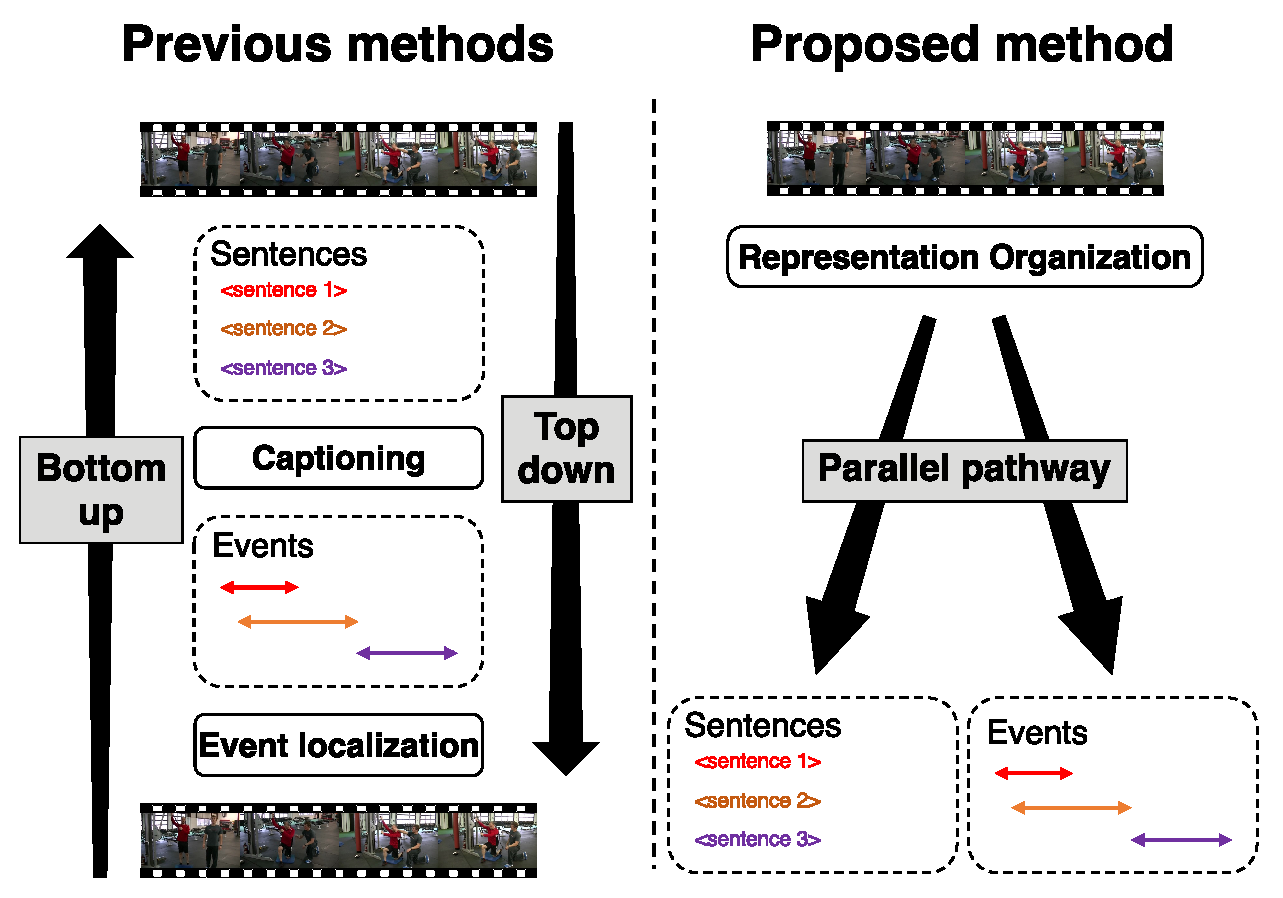
\includegraphics[width=\linewidth]{figures/ppvc_fig1}
  \caption{A summary of comparisons between existing methods and our approach to dense video captioning.}
  \label{fig:intro_approaches}
\end{figure}

\subsection{Limitations of Sequential Processing}

Sequential dense video captioning frameworks can be categorized into two primary paradigms: bottom-up and top-down approaches.
Bottom-up methods~\cite{krishna2017dense,li2018jointly,wang2018bidirectional,zhou2018end,mun2019streamlined} first detect temporal event proposals and subsequently generate corresponding captions, following a ``localize-then-describe'' pipeline.
Conversely, top-down approaches~\cite{deng2021sketch} generate paragraph-level descriptions and then ground individual sentences to specific temporal segments through a ``describe-then-localize'' strategy.

Both paradigms suffer from inherent architectural limitations that constrain their effectiveness.
The most critical issue is \textit{error propagation}: inaccuracies in the initial stage cascade to subsequent modules, creating a compounding effect that degrades overall performance.
In bottom-up approaches, poorly localized events inevitably lead to contextually inappropriate captions, regardless of the sophistication of the language generation module.
Similarly, top-down methods struggle when initial paragraph-level descriptions fail to capture essential temporal structures~\cite{wang2021end}.

Furthermore, sequential approaches typically require \textit{hand-crafted post-processing algorithms} such as Non-Maximum Suppression (NMS) for proposal selection \cite{hosang2017learning}.
These algorithms operate independently of video content, relying solely on temporal overlap criteria and predefined thresholds.
This content-agnostic processing often eliminates semantically meaningful events, particularly in scenarios involving multiple concurrent activities or nested temporal structures.

The sequential dependency also prevents \textit{end-to-end optimization}, necessitating complex multi-stage training procedures that hinder convergence and limit the model's ability to learn optimal joint representations for both localization and captioning tasks~\cite{zhou2018end,wang2021end}.

\subsection{Emergence of Parallel Processing}
Recognizing these fundamental limitations, recent research has explored parallel processing paradigms that perform event localization and caption generation simultaneously~\cite{wang2021end}.
Parallel approaches aim to eliminate sequential dependencies by employing shared encoder representations and parallel decoder heads for the two subtasks.

Wang et al.~\cite{wang2021end} introduced PDVC (Parallel Dense Video Captioning), which demonstrated that parallel decoding could significantly improve performance compared to sequential methods.
However, this pioneering work revealed new challenges specific to parallel architectures: \textit{information bottlenecks at branching points} and \textit{query limitation problems}.

The information bottleneck occurs because parallel approaches still maintain an ``encode-then-decode'' structure, where encoded video features must simultaneously serve both localization and captioning decoders.
This shared representation may not optimally capture the distinct information requirements of each subtask.
Additionally, the limited number of queries in transformer-based decoders restricts the maximum number of detectable events, particularly problematic for long videos containing multiple overlapping activities.

\subsection{Motivation for Enhanced Parallel Architecture}
Our analysis reveals that while parallel processing addresses the error propagation problem inherent in sequential approaches, current implementations fail to fully realize the potential of this paradigm.
The key insight driving our approach is that effective parallel processing requires not merely simultaneous decoding, but architectural innovations that eliminate information bottlenecks while preserving the rich contextual information necessary for both accurate localization and coherent caption generation.

To achieve this goal, we identify three critical design principles:
\begin{enumerate}
  \item Bottleneck-free Information Flow: Instead of forcing all information through a single bottleneck point, we propose passing comprehensive potential information at branching points and filtering unnecessary elements just before decoding. This approach ensures that both localization and captioning modules have access to the full spectrum of relevant visual and temporal information.
  \item Multi-scale Feature Integration: Recognizing that event localization and caption generation may benefit from different levels of feature abstraction, we introduce multi-stack cross-attention mechanisms that enable simultaneous access to both high-level semantic representations and low-level visual details~\cite{vaswani2017attention}.
  \item Dynamic Event Enumeration: Rather than predetermining the number of events through separate counter modules, we propose allowing the model to dynamically determine the optimal number of events based on video content, eliminating artificial constraints on event detection capability.
\end{enumerate}

As illustrated in Figure \ref{fig:intro_approaches}, our proposed Parallel Pathway Dense Video Captioning (PPVC) framework fundamentally reimagines the dense video captioning architecture by eliminating sequential dependencies while addressing the bottleneck limitations of existing parallel approaches.
Through these innovations, PPVC achieves superior performance in both temporal localization accuracy and caption quality compared to state-of-the-art sequential and parallel methods.

The remainder of this chapter details the architectural design and implementation of PPVC, demonstrating how these motivational insights translate into concrete algorithmic improvements that advance the state-of-the-art in dense video captioning.

\section{Parallel Pathway Architecture (PPVC)}
This section describes the core ideas and the network architecture of PPVC in detail.

\subsection{Overview}
For a given video, dense video captioning is the task of detecting multiple overlapping events and generating sentences accordingly.
Existing methods generally divide the whole process into two sub-problems, event detection, and sentence generation, and solve them one by one in order.
The performance of the two modules is tightly coupled, and this sequential processing method causes a major flaw: the result of the preceding module greatly affects the performance of the subsequent module.
However, parallel architectures have the challenge that the bottleneck of information at branch points can limit the outcomes.
Therefore, it is critical to decouple the dependency between the two modules by breaking the sequential processing paradigm while not occurring a bottleneck.

With this consideration, we construct two sub-problems of dense video captioning in parallel.
We first organize the encoded video features into highly relevant ones to understand the core context of the video, rather than directly generating events and sentences from the video.
PPVC consists of five modules: video encoder $\mathcal{E}$, representation organizer $\mathcal{O}$, event localizer $\mathcal{L}$, sentence generator $\mathcal{S}$, gating network $\mathcal{G}$ as depicted in Figure \ref{fig:architecture}. 

Given a video $\mathcal{V}$, it is converted to a hidden state vector $\mathbi{H}_v$ by the video encoder $\mathcal{E}$.
$\mathbi{H}_v$ is fed into the representation organizer $\mathcal{O}$ to organize the encoded video features that determine the context of the video storyline, which is the branch point of the parallel pathway without any bottleneck.
The event localizer $\mathcal{L}$ and sentence generator $\mathcal{S}$ then localize the events $\{e_i\}_{i=1}^{n}$ and generate sentences $\{s_i\}_{i=1}^{n}$, respectively, while further mitigating bottlenecks using multi-stack cross attention.
The gating network $\mathcal{G}$ controls the flow at branch points and refines information by blocking the flow of unnecessary event queries.
The procedure of PPVC is described in Algorithm~\ref{algo:ppvc}.

\begin{sidewaysfigure}
  \centering
   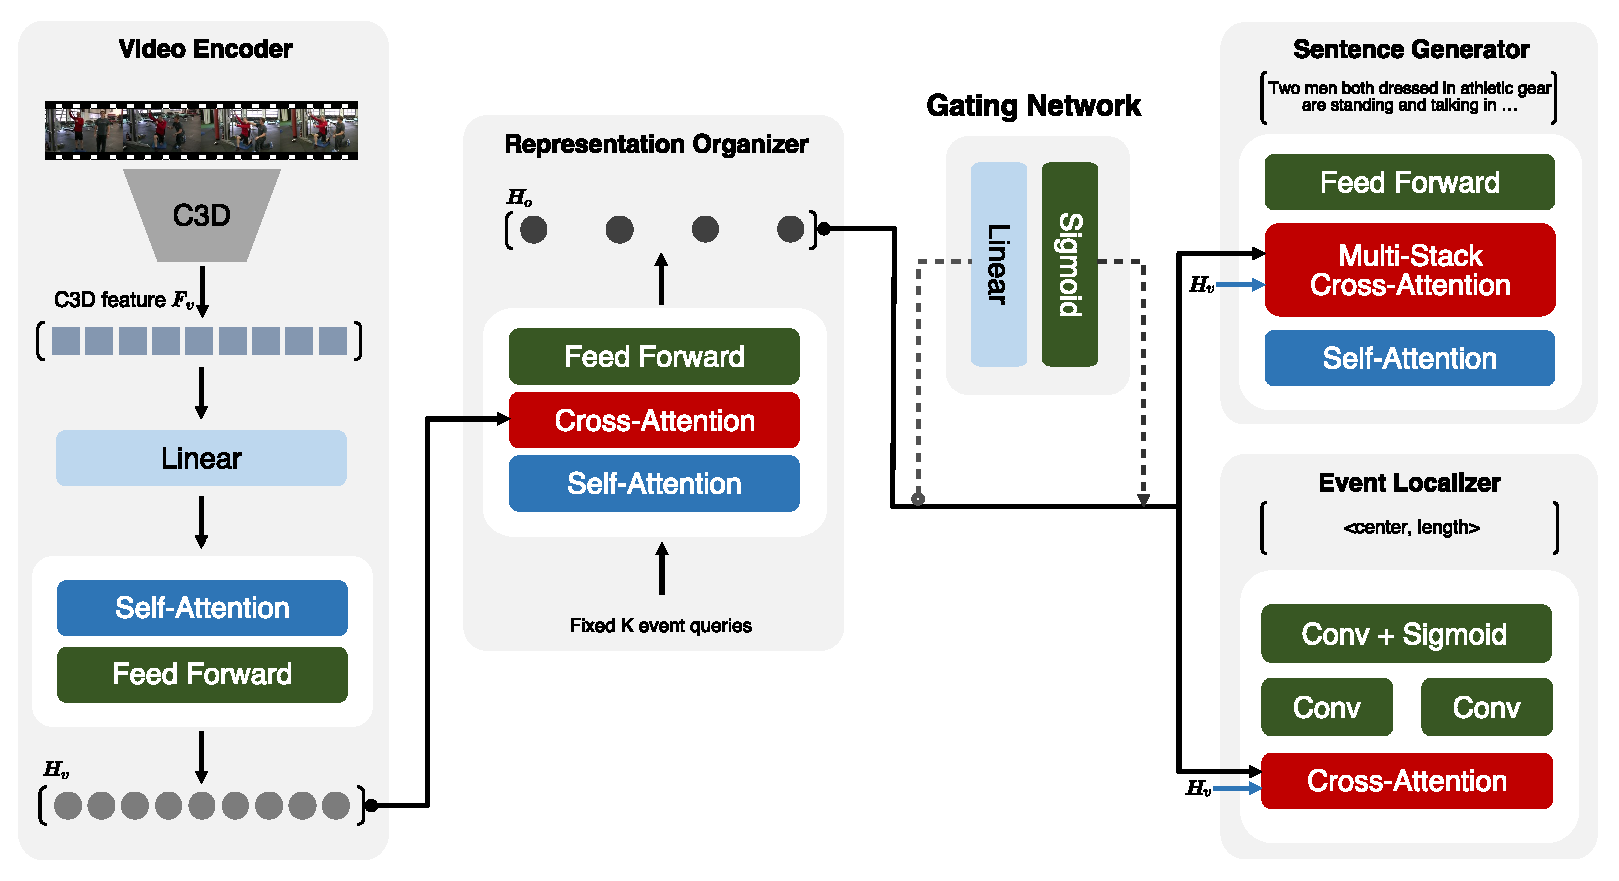
\includegraphics[width=\linewidth]{figures/ppvc_fig2}
   \caption{
    Architecture of the proposed method, PPVC.
   }
  \label{fig:architecture}
\end{sidewaysfigure}

% \begin{figure}[t]
%   \centering
%    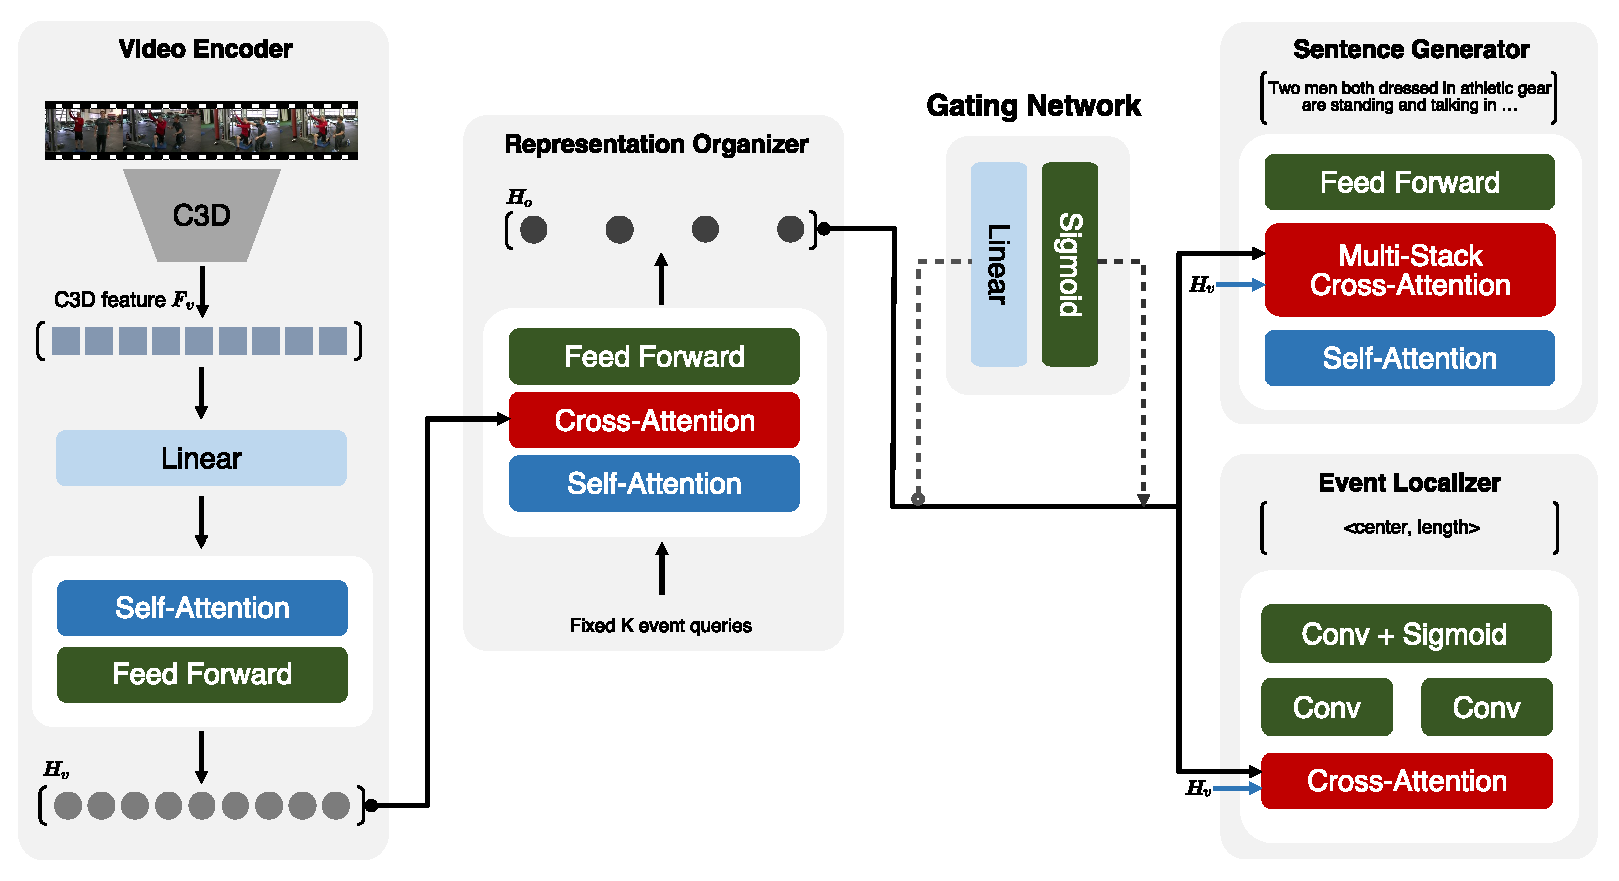
\includegraphics[width=\linewidth]{figures/ppvc_fig2}
%    \caption{
%     Architecture of the proposed method, PPVC.
%    }
%   \label{fig:architecture}
% \end{figure}

\subsection{Video Encoder}
The goal of the video encoder $\mathcal{E}$ is to extract the hidden state $\mathbi{H}_v$ by encoding the spatiotemporal context of the video $\mathcal{V}$.
Our video encoder consists of a convolution network and a sequential data encoder.
In particular, we adopt the C3D~\cite{tran2015learning} network and the transformer encoder~\cite{vaswani2017attention} with multi-head attention (MA) to understand the long-term temporal context of a video.
First, the video encoder divides a given video $\mathcal{V}$ into non-overlapping segments of fixed length (e.g., 8 frames).
The C3D network takes a segment as input and extracts features $\mathbi{F}_v \in \mathbb{R}^{T \times d_f}$, where $T$ is the number of segments and $d_f$ is the dimension of features.
We apply a linear transformation to feed the video feature $\mathbi{F}_v$ of dimension $d_f$ to the transformer encoder~\cite{vaswani2017attention} of dimension $d_m$ as follows:
\begin{equation}
  \mathbi{H}_v^0 = \text{PE} (\text{Linear} \left( \mathbi{F}_v \right) )
  \label{eq:linear_transformation}
\end{equation}
Then, after applying the positional encoding (i.e., $\text{PE}(\cdot)$) to $\text{Linear}(\bm{F}_v)$, we start with the input $\mathbi{H}_v^0$.

\begin{algorithm}[t]
  \caption{Parallel Pathway Dense Video Captioning}
  \label{algo:ppvc}
  \begin{algorithmic}[1]
    \STATE \textbf{Procedure} $\textsc{PPVC}(\mathcal{V})$
    \STATE $\mathbi{H}_v \gets \mathcal{E}(\mathcal{V})$ \COMMENT{Encode video}
    \FOR{$k = 1$ \TO $K$}
      \STATE $\mathbi{H}_o \gets \mathcal{O}(\mathbi{H}_v, \textbf{q}_k)$ \COMMENT{Organize features}
      \STATE $\mathbi{H}_o^{\text{gated}} \gets \mathbi{H}_o \times \mathcal{G}(\mathbi{H}_o)$ \COMMENT{Filter out}
      \STATE \COMMENT{Branch point!}
      \STATE $s_{k} \gets \mathcal{S}(\mathbi{H}_o^{\text{gated}}, \mathbi{H}_v)$ \COMMENT{Describe}
      \STATE $E_{k} \gets \mathcal{L}(\mathbi{H}_o^{\text{gated}}, \mathbi{H}_v)$ \COMMENT{Localize}
    \ENDFOR
    \RETURN $\{E_{k}\}_{k=1}^{K},\;\{s_{k}\}_{k=1}^{K}$
  \end{algorithmic}
\end{algorithm}

The transformer encoder, which contains multiple $N$ layers, is the core of our video encoder.
Each layer is made up of self-attention and feed-forward modules, and at the end of each module, there is a residual connection and layer normalization.
The transformer encoder outputs $\bm{H}_v^{l+1}$  in one cycle given $\mathbi{H}_v^l$, and the output of the last cycle---i.e., the last layer---is $\mathbi{H}_v$.
The following two equations can be used to describe the entire procedure:
\begin{equation}
  \mathbi{H}_v^{l+1} = \text{FFN}\left(\Psi \left(H_v^l + \text{MA}\left( \mathbi{H}_v^l, \mathbi{H}_v^l, \mathbi{H}_v^l \right) \right)\right)
  \label{eq:video_encoder_self_attention}
\end{equation}
\begin{equation}
  \text{FFN}(x) = \text{max} \left(0, x\mathbi{W}_1 + b_1 \right)\mathbi{W}_2 + b_2
  \label{eq:video_encoder_feed_forward}
\end{equation}
\begin{equation}
    \text{MA}(\bm{Q}, \bm{K}, \bm{V}) = \text{Cat}(\{\text{ATT}_i(\bm{Q}, \bm{K}, \bm{V})\}_{i=1}^h)W_O
  \end{equation}
  \begin{equation}
    \text{ATT}(\bm{Q}, \bm{K}, \bm{V}) = \text{softmax}( \frac{(\bm{QW}_Q)(\bm{K}\bm{W}_K)^T}{\sqrt{d_m}} ) (\bm{VW}_V)
  \label{eq:video_encoder_att}
\end{equation}
where, $\Psi\left(\cdot\right)$ represents the layer normalization function.
$\text{Cat}(\cdot)$ denotes vector concatenation and $\bm{W}_*$ are trainable parameters.
We repeat the above process as many times as the number of encoder layers.
Finally, the output of the video encoder is the output of the last layer $\mathbi{H}_v$.

Specifically, the multi-head attention module contains the following two classes of trainable parameters: $\bm{W}_{\{\bm{K},\bm{Q},\bm{V}\}}$ for the query ($\bm{Q}$), key ($\bm{K}$), and value ($\bm{V}$) attention matrix, and $\bm{W}_O$, which is in charge of the output by concatenating attention heads.
The attention head is calculated by scaled dot-product attention, as defined in Equation (\ref{eq:video_encoder_att}), with the same $\bm{H}_v^l$ being served into $\bm{K}$, $\bm{Q}$, and $\bm{V}$ for self-attention.
The final output of multi-head attention is then produced by concatenating all attention heads and applying the weight of $\bm{W}_O$. 
Two linear transformations and a ReLU \cite{agarap2018deep} activation function make up the feed-forward network $\text{FFN}(\cdot)$.
The first linear transformation (i.e., $\bm{W}_1$) and ReLU activation are applied to the output $x$ of multi-head attention. Then it goes through a second linear transformation (i.e., $\bm{W}_2$) with dropout as provided in Equation (\ref{eq:video_encoder_feed_forward}).

The representation organizer inherits the transformer's learning principle.
Specifically, with positional encoding and sequentially input video features, the transformer encoder learns the self-attention between features and organizes features for localization and captioning.
Intuitively, each hidden vector in the outputs of the transformer encoder implicitly contains information for localization and captioning. Therefore, by training in an end-to-end manner from the input to the localization and captioning heads, the representation organizer is trained toward the optimal.

\subsection{Representation Organization}
\label{subsec:method_representation_organization}
Before entering the parallel pathway, we introduce a representation organizer that organizes key encoded video features in the video's spatiotemporal context and uses them as intermediate information for event localization and sentence generation.
The goal of the representation organizer is to extract a representation of salient temporal regions in a video while implicitly producing all potential events.
Specifically, given a video $\mathcal{V}$, representation organizer outputs multiple representations $\mathbi{H}_o$ considering the entire video story.
Later, each representation serves as the core information for an event (i.e., timestamp and sentence), resulting in high-quality event localization and captioning.

For this, we adopt a query-based transformer decoder \cite{carion2020end,zhu2021deformable} because of its high performance and efficiency in object detection tasks using transformers \cite{vaswani2017attention}.
Given the $\mathbi{H}_v$ obtained by the video encoder and the input organized representation vector $\mathbi{H}_o^0$, the representation organizer computes the hidden state $\mathbi{H}_o$ as follows:
\begin{equation}
  \mathbi{H}_o^{\text{self}} = \Psi \left( \mathbi{H}_w^l + \text{MA} \left(\mathbi{H}_o^l, \mathbi{H}_o^l, \mathbi{H}_o^l \right) \right)
  \label{eq:representation_organization_self_attention}
\end{equation}
\begin{equation}
  \mathbi{H}_o^{\text{cross}} = \Psi \left( \mathbi{H}_o^{\text{self}} + \text{MA} \left( \mathbi{H}_o^{\text{self}}, \mathbi{H}_v, \mathbi{H}_v \right) \right)
  \label{eq:representation_organization_cross_attention}
\end{equation}
\begin{equation}
  \mathbi{H}_o^{l+1} = \Psi \left( \mathbi{H}_o^{\text{cross}} + \text{FFN}\left( \mathbi{H}_o^{\text{cross}} \right) \right)
  \label{eq:representation_organization_ffn}
\end{equation}
where, MA($\cdot$), FFN($\cdot$) and $\Psi \left(\cdot\right)$ are the same as used in Equation \ref{eq:video_encoder_self_attention} and Equation \ref{eq:video_encoder_feed_forward}.
$l$ is the sequence number of the transformer decoder.
The output of the last layer is $\mathbi{H}_o \in \mathbb{R}^{K \times d_m}$ ($K$ is the number of generated representations).

Here, as described above, we set the number of event queries to a fixed number of $K$ without depending on the event counter.
The event counter is likely to output the average number regardless of the content based on the statistics of the entire dataset.
We control the number of events by generating events for fixed $K$ event queries (i.e., the maximum number of events that PPVC can generate.) and removing unnecessary ones.

\textbf{Choice of $K$.}
Determining $K$ requires great care as it limits the maximum number of events that PPVC can generate.
With a high $K$, PPVC generates many events, so recall can be high, but precision is not guaranteed. 
On the other hand, a low $K$ increases precision, but does not guarantee high recall in videos containing many events.
Therefore, we empirically set $K$ to 10 to measure the F1 score by varying $K$ to strike the balance between recall and precision (details in Section \ref{subsec:experiments-ablation_study}).

\subsection{Event Localizer}
\label{subsec:method_event_localizer}
The goal of the event localizer is to predict the center and duration of an event in the video corresponding to an organized representation.
Common problems with the event localizer are that it is difficult to predict how many events are included in the video, and the events must be determined by considering the correlations between events.
Our event localization approach implicitly determines the number of events (i.e., the number of organized representations) in the previous step (representation organization), without an event counter or a proposal generation network.
Therefore, this section only focuses on the localization of the timestamps corresponding to the organized representations in the entire video.

The event localizer is based on the transformer decoder \cite{vaswani2017attention}.
The difference from the basic transformer decoder is that it does not have a self-attention block (i.e., not auto-regressive) and directly regresses the timestamp through several convolutional neural networks after the cross-attention block.
For each organized representation $\mathbi{H}_o$, we use a multi-head attention module to incorporate the entire video storyline (i.e., encoded video feature $\mathbi{H}_v$) as follows:
\begin{equation}
  \mathbi{H}_e^{\text{cross}} = \Psi \left( \mathbi{H}_e^{\text{self}} + \text{MA} \left( \mathbi{H}_e^{\text{self}}, \mathbi{H}_{v}, \mathbi{H}_{v} \right) \right)
  \label{eq:event_localizer_cross_attention}
\end{equation}
We then apply several 1D convolutional layers on the temporal dimension and predict the ratio of center and duration timestamps to the entire video using two linear regression heads.

\subsection{Sentence Generator}
\label{subsec:method-sentence_generator}
The goal of the sentence generator $\mathcal{S}$, the second part of the parallel pathway, is to receive organized representations $\{\mathbi{H}_o^i\}_{i=0}^{N}$ from the representation organizer and generate sentences ${\{s_i\}}_{i=0}^{N}$: $\mathcal{S}\left({\{\mathbi{H}_o^i\}_{i=0}^{N}}\right) \rightarrow {\{s_i\}}_{i=0}^{N}$.
One of the important points in sentence generation in a dense video captioning task is to maintain coherency.
There are several approaches to this, but we guarantee coherency between sentences by directly incorporating the textual features of the video.
Directly merging video features instead of merging past sentences improves sentence coherency while avoiding referencing ill-defined words in the last sentence.

Our sentence generator is based on a transformer decoder \cite{vaswani2017attention}, and most of the process is similar to $\mathcal{O}$.
The difference from the basic transformer decoder is that there are two hidden states (i.e., two pairs of key and value) that are input to the cross-attention block: the visual hidden state $\mathbi{H}_v$ and the organized representation $\mathbi{H}_o$.
Therefore, we design a multi-stack cross-attention module that refers to multiple hidden states.
This applies the multi-head attention module sequentially to two or more hidden states by stacking, which makes it possible to utilize various information during decoding.

The sentence generation process using multi-stack cross-attention is as follows:
\begin{equation}
  \mathbi{H}_s^{\text{cross}^1} = \Psi \left( \mathbi{H}_s^{\text{self}} + \text{MA} \left( \mathbi{H}_s^{\text{self}}, \mathbi{H}_{v}, \mathbi{H}_{v} \right) \right)
  \label{eq:setence_constructor_cross1_attention}
\end{equation}
\begin{equation}
  \mathbi{H}_s^{\text{cross}^2} = \Psi \left( \mathbi{H}_s^{\text{cross}^1} + \text{MA} \left( \mathbi{H}_s^{\text{cross}^1}, \mathbi{H}_{w}, \mathbi{H}_{w} \right) \right)
  \label{eq:setence_constructor_cross2_attention}
\end{equation}
Note that we omit positional encoding, self-attention, and feed-forward processes because they are the same as the representation organizer (Section \ref{subsec:method_representation_organization}).

\subsection{Gating Network}
\label{subsec:method-gating_network}
In addition to the modules described above, we employ a gating network that signals the end of a sequence of the representation organizer and controls the flow into parallel pathways.
Since the representation organizer creates all of the possible organized representations, it is necessary to prevent the generation of redundant or unnecessary events by indicating the end of the sequence and limiting the flow of parallel pathways.
In other words, the gating network consequently serves to increase precision in event localization.
Our gating network outputs a confidence score for the organized representation through the sigmoid activation function after linear transformation as follows:
\begin{equation}
  g(x) = \sigma (\text{Linear}(x))
\end{equation}
\begin{equation}
  \mathbi{H}_o^{\text{gated}} = g(\mathbi{H}_o) \cdot \mathbi{H}_o
  \label{eq:gating_network}
\end{equation}
It is simple but effective, prevents unnecessary representation generation, and as a result helps high-quality localization and captioning.

\section{Experimental Evaluation}
\subsection{Dataset}
\label{subsec:experiments-dataset}

% \begin{table*}[t]
\begin{sidewaystable}
  \centering
  \caption{
    Performance comparison of the event localization.
  }
  \begin{tabular}{@{}l|c|ccccc|ccccc|c@{}}
    \hline
    % Method & Recall (@tIoU) & Precision (@tIoU) \\
    % & \multicolumn{5}{l}{} & \multicolumn{5}{l}{} \\
    \multirow{2}{*}{Method} & \multirow{2}{*}{PN} & \multicolumn{5}{|c|}{Recall (@tIoU)} & \multicolumn{5}{c}{Precision (@tIoU)} & \multirow{2}{*}{F1} \\
    && @0.3 & @0.5 & @0.7 & @0.9 & Average & @0.3 & @0.5 & @0.7 & @0.9 & Average & \\
    \hline
    MFT'18 \cite{xiong2018move} & $\checkmark$ & 46.18 & 29.76 & 15.54 & 5.77 & 24.31 & 86.34 & 68.79 & 38.30 & 12.19 & 51.41 & 33.01 \\
    SDVC'19 \cite{mun2019streamlined} & $\checkmark$ & 93.41 & 76.40 & 42.40 & 10.10 & 55.58 & 96.71 & 77.73 & 44.84 & 10.99 & 57.57 & 56.56 \\
    PDVC'21 \cite{wang2021end} &  & 89.47 & 81.91 & 44.63 & 15.67 & 55.42 & 97.16 & 78.09 & 42.68 & 14.40 & 58.07 & 56.71 \\
    \textbf{PPVC} &  & 91.71 & 78.90 & \textbf{56.73} & \textbf{20.60} & \textbf{61.98} & 96.23 & 73.80 & 37.66 & 12.61 & 55.07 & \textbf{58.33} \\
    \hline
  \end{tabular}
  
  \label{tab:eval_event_localizer}
% \end{table*}
\end{sidewaystable}

% \begin{table*}[tp]
\begin{sidewaystable}
  \centering
  \caption{
    Performance comparison of the dense video captioning (ActivityNet Captions validation set).
  }
  \begin{tabular}{@{}l|ccc|cc|ccccccc@{}}
    \hline
    % Method & Recall (@tIoU) & Precision (@tIoU) \\
    % & \multicolumn{5}{l}{} & \multicolumn{5}{l}{} \\
    % \multirow{2}{*}{Method} & \multicolumn{6}{|c|}{with GT events} & \multicolumn{6}{c}{with predicted events} \\
    \multirow{2}{*}{Method} & \multicolumn{3}{|c|}{Feature} & \multicolumn{2}{|c|}{Training} \\
     & C3D & TSN & Optical & CE & RL & B@1 & B@2 & B@3 & B@4 & C & M\\
     \hline
    DCE'17 \cite{krishna2017dense}        & $\checkmark$ & & & $\checkmark$ & & 10.81 & 4.57  & 1.90  & 0.71 & 12.43 & 5.69\\
    TDA-CG'18 \cite{wang2018bidirectional} & $\checkmark$ & & & $\checkmark$ & & -     & -     & -     & 1.31  & 7.99 & 5.86\\
    DVC'18 \cite{li2018jointly}            & $\checkmark$ & & & $\checkmark$ & & 12.22 & 5.72  & 2.27  & 0.73 & 12.61 & 6.93\\
    Efficient'20 \cite{suin2020efficient}  & $\checkmark$ & & & $\checkmark$ & & -     & -     & 2.87  & 1.35 & 13.82 & 6.21\\
    ECHR'20 \cite{wang2020event}           & $\checkmark$ & & & $\checkmark$ & & -     & -     & -     & 1.29 & 14.71 & 7.19\\
    WS-DEC'21 \cite{chen2021towards}*      & $\checkmark$ & & & $\checkmark$ & & 13.36 & 5.96  & 2.78  & 1.33 & 21.21 & 7.49\\
    PDVC'21 \cite{wang2021end}             & $\checkmark$ & & & $\checkmark$ & & -     & -     & -     & 1.65 & 25.87 & 7.50 \\
    \textbf{PPVC}                       & $\checkmark$ & & & $\checkmark$ & & \textbf{14.93} & \textbf{7.40}  & \textbf{3.58}  & \textbf{1.68} & 23.02 & \textbf{7.91} \\
    \hline
    MT'18 \cite{zhou2018end} & & $\checkmark$ & $\checkmark$ & $\checkmark$   & & 9.96 & 4.81 & 2.42 & 1.15 & 9.25 & 4.98 \\
    SDVC'19 \cite{mun2019streamlined} & $\checkmark$ & & & $\checkmark$ & $\checkmark$ & 17.92 & 7.99 & 2.94 & 0.93 & 30.68 & 8.82 \\
    SGR'21 \cite{deng2021sketch} & $\checkmark$ & & & $\checkmark$ & $\checkmark$ & 14.05 & - & - & 1.67 & 22.12 & 9.07 \\
    \hline
  \end{tabular}
  \label{tab:eval_captioner}
% \end{table*}
\end{sidewaystable}

\begin{table}[tp]
  \centering
  \caption{
    Performance comparison of the dense video captioning (YouCook2-TSN).
  }
  \begin{tabular}{@{}l|c|c|cccc|ccccc|c@{}}
    \hline
    Method &  B@4 & C &  M \\
    \hline
    MT'18 \cite{zhou2018end} & 0.30 &  6.10 &  3.18 \\
    ECHR'18 \cite{wang2018bidirectional} & - & - &  3.82 \\
    PDVC'21 \cite{wang2021end} &  0.80 &  22.71 &  4.74 \\
    SGR'21 \cite{deng2021sketch} & - &  - &  4.35 \\
    \textbf{PPVC} &  \textbf{0.89} &  19.70 &  \textbf{4.94} \\
    \hline
  \end{tabular}
  \label{tab:eval_captioner_yc2}
\end{table}

We evaluate the performance of our framework on the two large-scale benchmark datasets, ActivityNet Captions \cite{krishna2017dense} and YouCook2 \cite{zhou2018towards}.
The ActivityNet Captions dataset contains 19,994 Youtube videos, which are divided into three subsets: 10,009, 4,917, and 4,885 videos for training, validation, and testing, respectively.
% We evaluate the performance of our framework on the ActivityNet Captions dataset \cite{krishna2017dense}, which contains 19,994 Youtube videos.
% They are divided into three subsets with 10,009, 4,917 and 4,885 videos for training, validation, and testing, respectively.
On average, the length of videos is 120 seconds, and each video has 3.65 pairs of events and sentences.
Each sentence has, on average, 13.48 words.
YouCook2 has 2,000 untrimmed videos of cooking activities with an average length of 320 seconds.
The videos have 7.7 events and sentences on average.
We use C3D \cite{tran2015learning} and TSN \cite{wang2018temporal} features for fair comparison for the ActivityNet Captions dataset and the YouCook2 dataset, respectively.
C3D features are obtained by passing non-overlapping, fixed-length video segments of 8 frames to the C3D network pre-trained on Sports-1M \cite{karpathy2014large}.

\subsection{Metrics}
\label{subsec:experiments-metrics}

We use publicly available evaluation code\footnote{\url{https://github.com/ranjaykrishna/densevid_eval}} provided by the ActivityNet Captions Challenge.
We measure recall and precision of event localization and METEOR \cite{banerjee2005meteor}, CIDEr \cite{vedantam2015cider} and BLEU \cite{papineni2002bleu} of sentences.
Given a generated event and sentence pair, if its event has an overlapping larger than the threshold with any ground-truth events, the captioning score is computed by comparing the corresponding ground-truth sentence.
Otherwise, the score is set to 0.


% METEOR is a widely used metric of the ActivityNet Captions challenge, but it tends to score high for redundant captions that are difficult for humans to read.
% METEOR inherently has a gap between what human prefer to read and what machines can generate.
% To circumvent such pitfall, we use SODA(c) \cite{fujita2020soda} as an evaluation metric, which is a story-oriented dense video captioning evaluation framework.
% SODA(c) is based on METEOR, however it penalizes duplicated captions.
% Thus, higher scores are given for captions that are equal to the number reference captions.
% We include SODA(c) because it reflects human readability better than METEOR.


\subsection{Implementation Details}
\label{subsec:experiments-impl_details}

For all modules, the hidden size $d_m$ of multi-head attention is 512, the number of attention heads is 8, and the encoder and decoder have 6 layers.
The feed-forward network used in the encoder and decoder is 2,048 dimensions.
The residual and attention dropout ratio is 0.1.
To prevent over-fitting, we apply dropout to the visual input embedding layer.
We train the model with adamW \cite{loshchilov2017decoupled} for 30 epochs with a batch size of 1.
We vary the learning rate as in \cite{vaswani2017attention} and set warmup steps to 10 epochs, which initially increases linearly from 0 to about 0.00005, and then decreases proportionally to the inverse square root.
The label smoothing factor is set to 0.1.

\subsection{Performance Comparison}
\label{subsec:experiments-perfom_comp}
We compare the performance of PPVC with several state-of-the-art methods \cite{krishna2017dense,wang2018bidirectional,li2018jointly,zhou2018end,mun2019streamlined,suin2020efficient,wang2020event,chen2021towards,deng2021sketch,wang2021end}.



\textbf{Event localization.}
We first compare the performance of the event localizer among the two subtasks and present the results in Table \ref{tab:eval_event_localizer}.
We evaluate the localization performance of PPVC with respect to the 4 temporal intersections of unions (@tIoU) thresholds on the Activity Captions validation set.
PN stands for proposal network.


MFT, SDVC, and PDVC explicitly detect events through the event proposal networks.
In contrast, our method uses the representation organizer to roughly compose representations of the events (i.e., implicit) and then localize each representation.
Our event localizer achieves superior performance over MFT, SDVC, and PDVC in terms of F1 score.
Specifically, PPVC surpasses MFT by a large margin, and although its precision is slightly lower than SDVC and PDVC, its recall is slightly superior, resulting in a higher F1 score.
Based on these results, we can confirm the effectiveness of the representation organizer, the event localizer, and the gating network without any proposal network.

\textbf{Dense video captioning.}
Tables \ref{tab:eval_captioner} and \ref{tab:eval_captioner_yc2} show the comparisons of captioning performance for state-of-the-art methods using BLEU@N (B@N), CIDEr (C) and METEOR (M) on the ActivityNet validation set and YouCook2 dataset, respectively.
Asterisk (*) indicates methods evaluated under an incomplete dataset (e.g., 80\%) due to a download issue.
CE and RL stand for cross-entropy and reinforcement learning, respectively.
PPVC achieves superior performance compared to the state-of-the-art scheme in terms of the widely used METEOR metric in the ActivityNet Captions challenge.

A few methods \cite{mun2019streamlined,deng2021sketch,wang2020event} adopt reinforcement learning to further improve performance after cross-entropy training.
They require extra-long training time for RL training and most importantly they tend to generate repetitive phrases \cite{wang2019describing}.
The RL fine-tuning approach expects high metric values but yields rather poor results in terms of human readability.
In short, metrics such as CIDEr and METEOR cannot perfectly evaluate human readability.
In this paper, since we attach great importance to both quantitative and qualitative results, we do not adopt the RL training in the language model.

\begin{table}[t]
  \centering
  \caption{
    A performance comparison of the dense video captioning with ground-truth proposals.
    % A summary of the performance comparison using BLEU@4 (B@4), CIDEr (C), and METEOR (M) with ground-truth proposals on the ActivityNet validation set.
  }
  \begin{tabular}{l|c|c|c}
    \hline
    Method & B@4 & C & M \\
    \hline
    DCE'17 \cite{krishna2017dense} & 1.60 & 8.88 & 25.12 \\
    TDA-CG'18 \cite{wang2018bidirectional} & - & 9.69 & - \\
    DVC'18 \cite{li2018jointly} & 1.62 & 10.33 & 25.24 \\
    ECHR'20 \cite{wang2020event} & 1.96 & 10.58 & 39.73 \\
    PDVC'21 \cite{wang2021end} & 2.64 & 10.54 & 47.26 \\
    \textbf{PPVC} & \textbf{2.76} & 10.48 & \textbf{49.31} \\
    \hline
  \end{tabular}
  \label{tab:eval_captioning_gt}
\end{table}

Note that, we exclude comparison methods that use anything other than C3D/TSN features (i.e., multi-modal) or train the captioning module with reinforcement learning after cross-entropy training.
RL adopts a natural language evaluation metric such as METEOR directly as a reward, which is very effective for high scores. 
However, it tends to generate repetitive phrases with long sentences \cite{wang2019describing}, which reduces readability \cite{wang2018bidirectional,fujita2020soda}.
In this work, we do not use the RL training in the language model since we place a high value on both quantitative and qualitative results.

We evaluate the PPVC with ground-truth proposals, examining only the captioning performance separately from event localization on the ActivityNet validation set, as shown in Table \ref{tab:eval_captioning_gt}.
Compared to other algorithms, PPVC is slightly inferior in CIDEr but superior in BLEU@4 and METEOR metrics, indicating that the events generated by PPVC are more accurate.
We also compare the performance of PPVC with the state-of-the-art methods on the YouCook2 dataset, as shown in Table \ref{tab:eval_captioner_yc2}.
Similarly, PPVC outperforms other algorithms in terms of METEOR and BLEU@4.
Based on these results, we can see that PPVC is effective with parallel pathways instead of sequential paradigms.
Compared to PDVC, which is a similar parallel decoding approach, PPVC achieves slightly better results in terms of BLEU and METEOR, indicating the effectiveness of representation organizers over event counter head.

We analyze PPVC in depth based on the evaluation mechanisms and values of the metrics.
CIDEr (Consensus-based Image Description Evaluation) is a TF-IDF (Term Frequency-Inverse Document Frequency)-based natural language evaluation metric.
By taking into account both the frequency of the words and the length of the document, TF-IDF determines the importance of each word.
CIDEr evaluates a candidate sentence by vectorizing the TF-IDF values of words in the candidate sentence and reference sentences and comparing their similarity.
Intuitively, it tends to ignore grammar and word order and concentrate more on event-specific words than common words in reference sentences.
METEOR (Metric for Evaluation of Translation with Explicit ORdering), on the other hand, evaluates a candidate sentence using a penalty function for inconsistencies and weighted F-score (i.e., both recall and precision).
It takes into account the portion of the generated sentence where the n-grams match those of the reference sentences.
We contend, based on these facts, that PPVC has advantages in terms of sentence completeness using common words and drawbacks in generating event-specific words.

\begin{table}[t]
  \centering
  \caption{
    Average number of events per video.
    % Average number of events per video generated by the event localizer on ActivityNet Caption validation set.
    % PN, NMS and EC are proposal network, non-maximum suppression and event counter, respectively.
  }
  \begin{tabular}{l|c|c}
    \hline
    Method & Approach & Num. events \\
    \hline
    SDVC'19 \cite{mun2019streamlined} & PN+NMS & 2.85 \\
    PDVC'21 \cite{wang2021end} & EC & 3.03\\
    \textbf{PPVC} & - & 5.54 \\
    % Avg. number of GT events & & 3.65 \\
    \hline
  \end{tabular}
  \label{tab:eval_num_events}
\end{table}

\begin{figure}[t]
  \centering
%   \includegraphics[width=0.9\linewidth]{figures/distribution_num_events}
   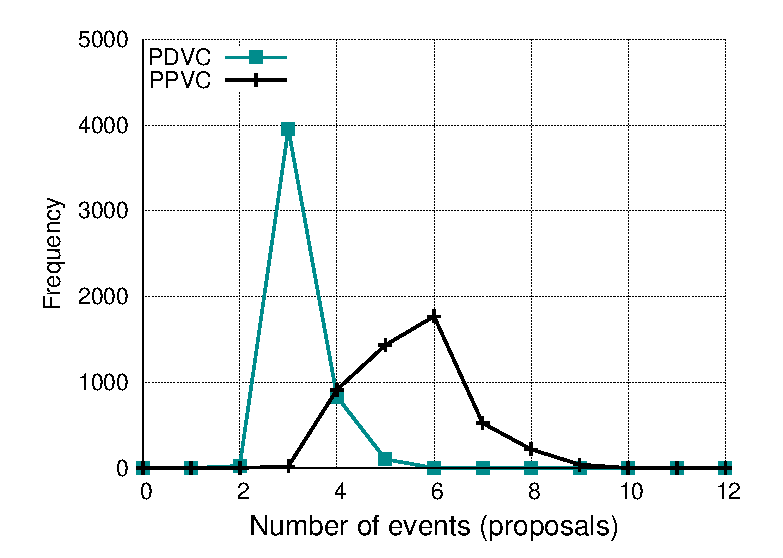
\includegraphics[width=0.9\linewidth]{figures/ppvc_fig3}
   \caption{
    Distribution of the number of events per video.
    % Distribution of the number of events generated by PDVC and PPVC.
    % PPVC generates more events and sentences on average, indicating a richer description of the video.
   }
   \label{fig:eval_dist_events}
\end{figure}

\textbf{Representation organization.}
For a more in-depth analysis of representation organizers, we examine the events generated from all videos included in the ActivityNet Captions validation set.
Table \ref{tab:eval_num_events} and Figure \ref{fig:eval_dist_events} show the number of events generated from each method, and the distribution of the number of events generated for all videos, respectively.
In Table {\ref{tab:eval_num_events}}, PN, NMS, and EC are proposal network, non-maximum suppression, and event counter, respectively.

In PPVC, the number of events is widely distributed from 3 to 9, whereas PDVC generates only 3 to 5 events per video.
In terms of the average number, PPVC, PDVC, and SDVC generate 5.54, 3.03, and 2.85 events, respectively, indicating that PPVC generates more sentences and a more detailed description of the video.

Furthermore, based on the above results, the event counter of PDVC outputs 3 (80.4 \%), which is the average of the number of events of the videos in the entire dataset.
On the other hand, PPVC without an event counter generates proposals with a more diverse number of events.





\begin{figure}[t]
  \centering
%   \includegraphics[width=0.9\linewidth]{figures/eval_ablation}
   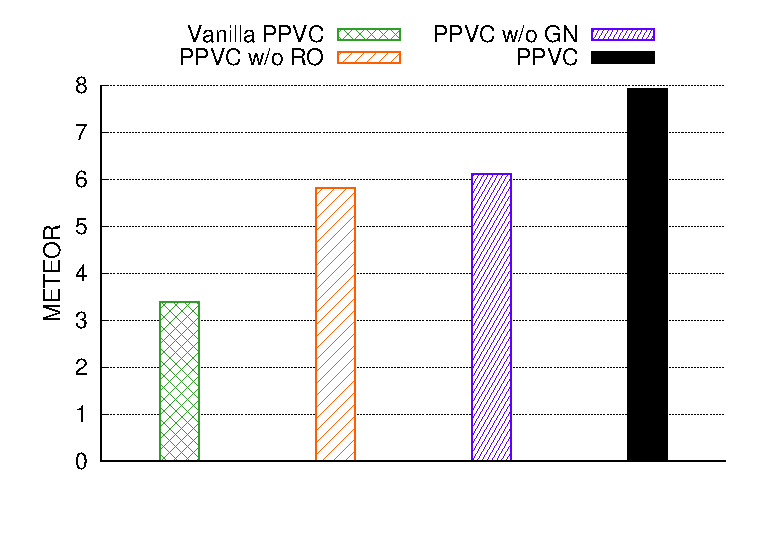
\includegraphics[width=0.9\linewidth]{figures/ppvc_fig4}
   \caption{
    The ablation result of each module for captioning.
    % Ablation results on ActivityNet Captions validation set.
    % Vanilla PPVC means a simple parallel pathway model without both the representation organizer and the gating network used in the full model.
    % ``RO" and ``GN" stand for the representation organizer and the gating network, respectively.
    }
   \label{fig:eval_ablation}
   \end{figure}

\begin{table}[t]
   \centering
   \caption{
      The ablation result of each module for localization.
    %   Ablation results of average recall and precision on the ActivityNet Captions validation set.
    %   Vanilla PPVC means a simple parallel pathway model without the representation organizer and the gating network used in the full model.
    % ``RO" and ``GN" stand for the representation organizer and the gating network, respectively.
   }
   \begin{tabular}{l|c|c}
      \hline
      Method & Recall & Precision \\
      \hline
      Vanilla    & 44.53 & 32.92 \\
      W/o RO    & 77.90 & 34.57 \\
      W/o GN    & 74.37 & 39.93 \\
      Full       & 61.98 & 58.33 \\
      \hline
  \end{tabular}
  \label{tab:eval_ablation_event_localization}
 \end{table}
 


\subsection{Ablation Study}
\label{subsec:experiments-ablation_study}
\textbf{Ablation study on each module.}
We conduct several ablation studies to precisely quantify the contribution of the core modules of PPVC.
We compare the performance of 4 different models with different combinations of modules as follows: (i) vanilla PPVC: has a parallel pathway but no representation organizer and gating network, (ii) PPVC without representation organizer: directly localizes and describes the events from the encoded video, (iii) PPVC without gating network: does not control the flow to the event localizer and the sentence generator, (iv) PPVC (full model).

Figure {\ref{fig:eval_ablation}} and Table {\ref{tab:eval_ablation_event_localization}} show the average recall and precision (i.e., localization) of an ablation study on the ActivityNet validation set and we have the following observations.
``RO" and ``GN" stand for the representation organizer and the gating network, respectively.
First, vanilla PPVC eliminates the dependency between the two modules with a parallel architecture, however, suffers from localizing and describing events directly from the vast amounts of video features.
We argue that the simple parallel pathway dense video captioning model may not be as effective as the conventional sequential method.
Second, applying the representation organizer to vanilla PPVC, it can be seen that there is a significant performance gain.
This result proves that the representation organizer acts as a filter to extract only the necessary (core) information and guides the event localizer and sentence generator.
Third, the gating network is essential in PPVC because it controls the flow from the representation organizer to the parallel pathway and filters the unnecessary representations.
%

\begin{figure}[t]
  \centering
%   \includegraphics[width=0.9\linewidth]{figures/eval_ablation_num_query.eps}
   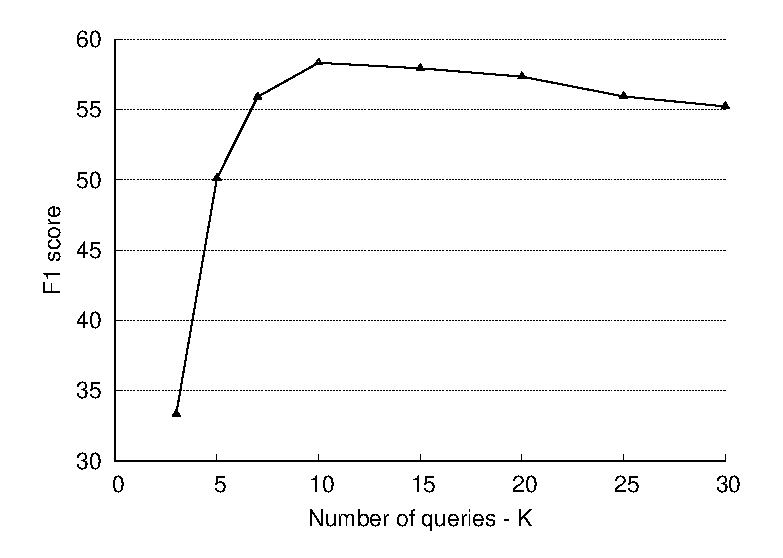
\includegraphics[width=0.9\linewidth]{figures/ppvc_fig5}
   \caption{
    The ablation result of the number of queries.
    % Ablation results on ActivityNet Captions validation set.
    % We measure the F1 score by varying $K$, the number of fixed queries in PPVC.
   }
   \label{fig:eval_ablation_num_query}
\end{figure}



\textbf{Ablation study on the number of queries.}
We train several times to determine the number of fixed queries, $K$, and measure F1 for the generated events by varying $K$.
Based on the fact that the ActivityNet Captions dataset contains videos of up to 27 events, we examine the results for $K$ of 3, 5, 7, 10, 15, 20, 25, and 30.
It can be seen that the best performance is when the number of queries is 10, as shown in Figure \ref{fig:eval_ablation_num_query}.
The overall performance tends to improve as the number of queries rises, but when it exceeds 10, it starts to somewhat decline.
PPVC has the following trade-offs, depending on the number of queries: Low query numbers cause PPVC to have a low recall in event localization; on the other hand, high query numbers cause a high recall but poor precision.
Consequently, we set $K$ to 10 for the number of queries, which is the best F1 score (i.e., the harmonic mean of the recall and precision).

In short, by eliminating bottlenecks caused by the representation organizer and the gating network, PPVC achieves performance improvements over PDVC, an existing parallel decoding method.
Figure \ref{fig:eval_ablation} demonstrates the efficiency of the representation organizer and the gating network, while Figure \ref{fig:eval_ablation_num_query} demonstrates the need for a larger number of queries.

\begin{sidewaysfigure}
\centering
  % \fbox{\rule{0pt}{5in} \rule{1\linewidth}{0pt}}
%  \includegraphics[width=1\linewidth]{figures/eval_qualitative}
  \includegraphics[width=0.8\columnwidth]{figures/ppvc_fig6}
  \caption{
    Examples of qualitative results on ActivityNet Captions validation set.
    Sentences corresponding to the event are matched with the same color.
  }
  \label{fig:eval_qualitative_results}
\end{sidewaysfigure}

% \begin{figure*}[!tp]
%   \centering
%   % \fbox{\rule{0pt}{5in} \rule{1\linewidth}{0pt}}
% %  \includegraphics[width=1\linewidth]{figures/eval_qualitative}
%   \includegraphics[width=1\linewidth]{figures/ppvc_fig6}
%   \caption{
%     Examples of qualitative results on ActivityNet Captions validation set.
%     Sentences corresponding to the event are matched with the same color.
%   }
%   \label{fig:eval_qualitative_results}
% \end{figure*}

\subsection{Qualitative Results}
\label{subsec:experiments-qual_res}

Figure \ref{fig:eval_qualitative_results} illustrates the qualitative results of localizing and describing events in the video.
First, it can be seen that PPVC localizes and describes videos with a large number of events (i.e., more than 4) in both examples.
To detect more events, PPVC has two mechanisms: the representation organizer (Section \ref{subsec:method_representation_organization}) and the gating network (Section \ref{subsec:method-gating_network}).
The representation organizer implicitly generates all possible events based on the number of queries.
Then, the gating network eliminates unnecessary events to determine the final events of PPVC.

Second, We can see that PPVC generates fluent and rich sentences using the keywords such as ``kayak'', ``waves'', ``bumpy'', ``dog'', ``man'', ``frisbee'' and ``catch'' in both examples.
Unfortunately, there are some ill-defined sentences in the black and pink sentences in the second video.
PPVC generates the same sentence for two different events.
However, generating repeated sequences is one of the common challenges of language models.
We leave reducing this by contributing to sentence generation as our future work.

\section{Advantages and Limitations}
\label{sec:advantages_limitations}

The Parallel Pathway Dense Video Captioning (PPVC) framework introduces significant architectural innovations that address fundamental limitations of sequential processing paradigms while introducing new challenges inherent to parallel transformer-based architectures. This section provides a comprehensive analysis of the advantages and limitations of our proposed approach.

\subsection{Advantages}

\textbf{Elimination of Error Propagation.}
The most significant advantage of PPVC lies in its ability to eliminate the error propagation problem that plagues sequential dense video captioning methods~\cite{Krishna2017-pw,Li2018-ll,Wang2018-ap}.
By performing event localization and caption generation simultaneously rather than sequentially, PPVC prevents localization errors from cascading to the captioning module.
This architectural design ensures that both subtasks have access to the same rich visual representations, enabling more robust and accurate dense video captioning performance as demonstrated in our experimental results.

\textbf{Bottleneck-Free Information Flow.}
Traditional parallel approaches suffer from information bottlenecks at branching points where encoded features must serve both localization and captioning decoders~\cite{Wang2021-zi}. PPVC addresses this limitation through its representation organizer module, which extracts comprehensive potential information before branching and filters unnecessary elements just before decoding. This design ensures that both pathways receive rich, contextually relevant features without artificial constraints imposed by limited intermediate representations.

\textbf{Enhanced Feature Utilization through Multi-Stack Cross-Attention.}
The multi-stack cross-attention mechanism represents a key innovation that enables simultaneous access to both organized high-level features and raw low-level visual information~\cite{Vaswani2017-sc}. This dual-pathway feature utilization addresses the limitation that individual attention heads may focus on different aspects of the input, allowing the model to leverage complementary information sources for improved localization and captioning accuracy. The parallel processing of multi-head attention mechanisms provides computational efficiency while maintaining the model's ability to capture complex temporal relationships~\cite{Dosovitskiy2021-vn}.

\textbf{Content-Aware Event Detection.}
Unlike conventional approaches that rely on hand-crafted algorithms such as Non-Maximum Suppression (NMS)~\cite{hosang2017learning}, PPVC employs a gating network that makes content-aware decisions about event relevance. This eliminates the risk of removing semantically important but temporally overlapping events, which is particularly crucial for complex video scenarios where multiple concurrent activities occur. Our results demonstrate that PPVC generates significantly more events per video (5.54 vs. 3.03 for PDVC), enabling richer and more detailed video descriptions.

\textbf{End-to-End Optimization.}
The parallel architecture enables true end-to-end optimization without the complex multi-stage training procedures required by sequential methods~\cite{Zhou2018-zu}. This unified training approach allows the model to learn optimal joint representations for both localization and captioning tasks, leading to improved overall performance and training stability.

\subsection{Limitations}
\textbf{Fixed Query Limitations and Scalability Constraints.}
A fundamental limitation of PPVC lies in its reliance on a fixed number of queries ($K=10$) to determine the maximum number of detectable events.
This design choice creates an inherent trade-off between recall and precision: low query numbers limit recall for videos with many events, while high query numbers may decrease precision due to false positive generation. Although our empirical analysis determined the optimal value through F1 score optimization, this constraint may limit the framework's applicability to videos with highly variable event densities or exceptionally complex temporal structures.

\textbf{Computational Complexity and Memory Requirements.}
The transformer-based architecture, while enabling parallel processing, introduces significant computational overhead due to the quadratic complexity of self-attention mechanisms~\cite{Vaswani2017-sc}. Specifically, the computational complexity scales as $O(n^2 \cdot d + n \cdot d^2)$, where n represents the sequence length and d denotes the feature dimension.
This quadratic scaling in both time and memory requirements can become prohibitive for long video sequences, particularly when processing untrimmed videos that may contain hundreds or thousands of temporal segments. Recent work has established theoretical lower bounds proving that self-attention complexity is necessarily quadratic unless strong computational assumptions are violated~\cite{duman2023computational}.

\textbf{Residual Sequential Characteristics.}
Despite the parallel decoding architecture, PPVC maintains an encoding-then-decoding structure that preserves some sequential characteristics. The video encoder processes the entire input sequence before parallel pathways begin operation, potentially creating a bottleneck where poorly encoded features can negatively impact both localization and captioning performance. This limitation suggests that future architectures might benefit from more thoroughly parallel processing that extends to the encoding stage.

\textbf{Caption Generation Quality and Diversity.}
Our qualitative analysis reveals that PPVC occasionally generates repetitive captions for distinct events, particularly in scenarios with similar visual content but different semantic contexts.
This limitation reflects a broader challenge in neural language generation where models may converge to high-probability but less diverse outputs~\cite{wang2019describing}.
The repetitive caption problem is exacerbated by the parallel generation process, which lacks the sequential context that might help differentiate between similar events.

\textbf{Memory Allocation and Hardware Constraints.}
The multi-stack cross-attention mechanism and large query sets require substantial GPU memory, potentially limiting deployment in resource-constrained environments.
Modern transformer architectures typically face sequence length limitations of approximately 512 tokens due to memory constraints~\cite{tay2022efficient}, which may restrict PPVC's applicability to extremely long video sequences without additional optimization techniques such as gradient checkpointing or attention approximations.

\textbf{Limited Adaptability to Variable Event Complexity.}
The framework's performance is optimized for datasets with specific event density distributions, as evidenced by the empirical determination of $K=10$ based on ActivityNet Captions statistics.
This specialization may limit generalizability to video domains with significantly different temporal structures, such as surveillance footage with sparse events or highly dynamic content with continuous action sequences.

\subsection{Future Directions for Improvement}
The identified limitations suggest several promising directions for future research. Adaptive query mechanisms that dynamically adjust the number of queries based on video content could address the fixed query limitation. Advanced attention approximation techniques, such as linear attention variants or sparse attention patterns, could mitigate computational complexity while preserving model effectiveness. Additionally, incorporating more sophisticated caption diversification strategies during training could reduce repetitive generation issues and improve overall caption quality.
% !TEX root = main.tex

\chapter{Weakly Supervised Dense Video Captioning with Pretraining}
\label{chap:pws_dvc}

\section{The Challenge of Limited Annotations}

The advancement of dense video captioning has been significantly constrained by the fundamental challenge of limited annotated datasets, which poses critical obstacles for developing robust and generalizable models. While recent progress in parallel processing approaches~\cite{Wang2021-zi,Choi2022-cu} has addressed architectural bottlenecks and error propagation issues, these methods continue to rely heavily on fully supervised learning with expensive temporal annotations that require precise event boundaries and corresponding natural language descriptions.

The scarcity of densely annotated video datasets presents a multifaceted challenge that extends beyond simple data quantity. Current datasets such as ActivityNet Captions~\cite{Krishna2017-pw} and YouCook2~\cite{Zhou2018-eq} contain only 20,000 and 2,000 videos respectively, which pales in comparison to the millions of video-text pairs available in large-scale clip-level datasets~\cite{Miech2019-hk,Bain2021-si,Xu2016-ti}. The annotation process for dense video captioning requires human annotators to precisely identify temporal boundaries for multiple overlapping events and generate corresponding captions, making it substantially more expensive and time-consuming than clip-level video captioning tasks~\cite{Chen2011-ai,Wang2019-tk}.

\textbf{Annotation Dependency in Current Approaches.}
Despite architectural innovations in recent dense video captioning methods, including parallel processing frameworks~\cite{Wang2021-zi,Choi2022-cu} and transformer-based approaches~\cite{Zhou2018-zu,Lin2022-wi}, the fundamental reliance on dense temporal annotations remains unchanged. These methods require ground-truth event boundaries and caption pairs for effective training, creating a significant bottleneck for scaling to larger and more diverse video collections. Even sophisticated approaches that employ multi-modal fusion~\cite{Iashin2020-ln,Rahman2019-rp} or hierarchical processing~\cite{Deng2021-qd} cannot circumvent this annotation dependency, limiting their practical applicability in real-world scenarios where extensive manual annotation is prohibitive.

The annotation challenge becomes particularly acute when considering the nondeterministic nature of event interpretation illustrated in Figure~\ref{fig:nondeterminism}. Different annotators may identify distinct temporal boundaries and generate diverse captions for identical video content, introducing variability that compounds the difficulty of creating consistent training datasets~\cite{Summers2021-mz}. This subjectivity in human annotation not only increases the cost of dataset creation but also raises questions about the reliability and generalizability of models trained on such data.

\begin{figure}[t]
    \centering
    \includegraphics[width=\columnwidth]{figures/pws_introduction_nondeterminism}
    \caption{Example of dense video captioning for a video extracted from the ActivityNet Captions dataset.
        Note the different definitions of events and captions for the same video, highlighting the nondeterministic nature of human annotation.}
    \label{fig:nondeterminism}
\end{figure}

\textbf{Limitations of Current Pretraining Approaches.}
Recent efforts to address annotation scarcity through large-scale pretraining~\cite{Yang2023-fm,Zhang2022-ni,Seo2022-ok} have shown promise but face inherent limitations. Methods like Vid2Seq~\cite{Yang2023-fm} leverage narrated video datasets with automatically transcribed speech, but these approaches suffer from temporal misalignment between narration and visual events, particularly in videos with limited or no speech content. Similarly, approaches that utilize automatically generated pseudo-events~\cite{Zhang2022-ni} often produce noisy supervision signals that may not transfer effectively to downstream dense captioning tasks.

The fundamental challenge lies in bridging the gap between abundant clip-level video-text datasets and the sparse event-level annotations required for dense video captioning. While clip-level datasets contain millions of video-caption pairs that could potentially inform dense captioning models, existing approaches have struggled to effectively leverage this wealth of data due to the mismatch between clip-level and event-level supervision signals.

\textbf{Promise of Weakly Supervised Learning.}
Weakly supervised approaches~\cite{Duan2018-qf,Chen2021-sv,Rahman2019-rp} offer a promising alternative by learning from video-level captions without requiring explicit temporal annotations. However, existing weakly supervised methods face a critical limitation: their performance is heavily dependent on the quality of the captioning module, creating a chicken-and-egg problem where poor captions lead to ineffective localization, which in turn degrades caption quality.

The key insight motivating our approach is that the abundance of high-quality clip-level video captioning datasets~\cite{Xu2016-ti,Bain2021-si,Wang2019-tk} can be strategically leveraged to pretrain robust captioning modules that subsequently enable effective weakly supervised dense video captioning. Unlike fully supervised methods that require expensive event-level annotations, or existing pretraining approaches that rely on noisy automatically generated data, our strategy harnesses the wealth of human-annotated clip-level datasets to bootstrap dense video captioning capabilities.

\begin{figure}[t]
    \centering
    \includegraphics[width=\columnwidth]{figures/pws_Introduction_approach}
    \caption{The approach of the proposed method. Our technique addresses annotation scarcity by pretraining the event captioning module on abundant clip-level datasets, then fine-tuning through weakly supervised learning.
        CL and EC stand for caption localization and event captioning, respectively.}
    \label{fig:approach}
\end{figure}

\textbf{Motivation for PWS-DVC.}
Our proposed PWS-DVC framework, illustrated in Figure~\ref{fig:approach}, addresses the annotation challenge through a two-stage approach that maximizes the utilization of available data while minimizing dependence on expensive temporal annotations. By pretraining the event captioning module on large-scale clip-level datasets and subsequently fine-tuning through weakly supervised learning, PWS-DVC enables effective dense video captioning without requiring the extensive event-level annotations that constrain existing approaches.

This strategy offers several key advantages: (1) it leverages the vast amount of clip-level video-text data already available, (2) it reduces the annotation burden by eliminating the need for precise temporal boundaries during training, and (3) it enables better generalization by learning from diverse video content across multiple domains. The resulting framework demonstrates that effective dense video captioning can be achieved through careful utilization of existing data resources rather than requiring extensive new annotations.

\begin{sidewaysfigure}
    \centering
    \includegraphics[width=\textwidth]{figures/pws_network_architecture}
    \caption{Network architecture of the proposed model, PWS-DVC.
        PWS-DVC consists of two modules: caption localization and event captioning.
        The caption localization module takes a video and a caption as input and aims to localize which temporal region the caption corresponds to in the video.
        The event captioning module aims to generate a sentence describing the event given a video and its event.
        Both modules enable dense video captioning by alternatively training with video and ground-truth captions without supervision on events.}
    \label{fig:net_archi}
\end{sidewaysfigure}
% \begin{figure}[t]
%     \centering
%     \includegraphics[width=\textwidth]{figures/pws_network_architecture}
%     \caption{Network architecture of the proposed model, PWS-DVC.
%         PWS-DVC consists of two modules: caption localization and event captioning.
%         The caption localization module takes a video and a caption as input and aims to localize which temporal region the caption corresponds to in the video.
%         The event captioning module aims to generate a sentence describing the event given a video and its event.
%         Both modules enable dense video captioning by alternatively training with video and ground-truth captions without supervision on events.}
%     \label{fig:net_archi}
% \end{figure}

\section{PWS-DVC Framework}

\subsection{Overview}
Our proposed method, PWS-DVC, addresses the constraint of existing dense video captioning methods, which rely on specialized datasets for dense video captioning, such as ActivityNet Captions~\cite{Krishna2017-pw}.
Instead, we leverage weakly supervised dense video captioning to its maximum capacity by pretraining on readily accessible datasets for video clip-level captioning.
As depicted in Figure~\ref{fig:net_archi}, PWS-DVC comprises two distinct modules, namely the caption localization module and the event captioning module.
The module for captioning localization is responsible for determining the specific temporal interval in a video where a particular caption is positioned. On the other hand, the event captioning module is designed to construct a phrase that describes a video clip based on the provided video and event.
To address the difficulty of dense video captioning, we employ a two-step approach. Firstly, we pretrain the event captioning module using video clip-level datasets.
Subsequently, the two modules are trained in an alternating manner.

\begin{algorithm}
    \caption{Training procedure of PWS-DVC.}
    \begin{algorithmic}[1]
        \renewcommand{\algorithmicrequire}{\textbf{Input:}}
        \renewcommand{\algorithmicensure}{\textbf{Output:}}
        \REQUIRE $\mathcal{D}_\text{MSR-VTT}, \mathcal{D}_\text{ANetC}$ // datasets used for training
        \REQUIRE $\mathcal{C}, \mathcal{G}$ // event captioning and caption localization modules
        \REQUIRE $\left\{\boldsymbol{E}_j^{(a)}\right\}_{j=0}^{N_a}$ // anchors for training $\mathcal{G}$
        \REQUIRE $E^{(0.5,1)}$ // event that covers the entire video.
        \ENSURE  $\theta_\mathcal{C}$, $\theta_\mathcal{G}$ // trained parameters
        \\ Pretrain procedure
        \FOR {($\bm{V},\{C_i\}_{i=0}^{N_v}) \in \mathcal{D}_\text{MSR-VTT}$}
        \STATE $C = \textit{ChooseOne}(\{C_i\}_{i=0}^{N_v})$
        \STATE $C^\prime = \mathcal{C}(V, E^{(0.5,1)})$
        \STATE $\mathcal{L}_c = \textit{CrossEntropy}(C, C^\prime)$
        \STATE $\theta_\mathcal{C} = \theta_\mathcal{C} - \eta_\mathcal{C} \frac{\partial \mathcal{L}_c}{\partial \theta_\mathcal{C}}$
        \ENDFOR
        \\ Fine-tuning procedure
        \FOR {($\bm{V},\{C_i\}_{i=0}^{N_v}) \in \mathcal{D}_\text{ANetC}$}
        \STATE $C = \textit{ChooseOne}(\{C_i\}_{i=0}^{N_v})$
        \STATE $E^\prime, \text{confidence} = \mathcal{G}(V,C+\delta)$
        \STATE $C^\prime = \mathcal{C}(V,E^\prime)$
        \STATE $E^{\prime\prime} = \mathcal{G}(V,C^\prime)$
        \STATE $\{C_j\}_{j=0}^{N_a} = \{\mathcal{G}(V, E_j)\}_{j=0}^{N_a}$
        \STATE $\{\text{score}_j\}_{j=0}^{N_a}=\{\text{METEOR}(C,C_j)\}_{j=0}^{N_a}$
        \STATE $\text{best}=\text{argmax}_j\{\text{score}_j\}_{j=0}^{N_a}$
        \STATE $\mathcal{L}_c = \textit{CE}(C, C^\prime)$
        \STATE $\theta_\mathcal{C} = \theta_\mathcal{C} - \eta_\mathcal{C} \frac{\partial \mathcal{L}_c}{\partial \theta_\mathcal{C}}$
        \STATE $\mathcal{L}_l = \textit{MSE}(E^\prime, E^{\prime\prime}) + \textit{CE}(\text{confidence, \text{best}})$
        \STATE $\theta_\mathcal{G} = \theta_\mathcal{G} - \eta_\mathcal{G} \frac{\partial \mathcal{L}_l}{\partial \theta_\mathcal{G}}$
        \ENDFOR
        \RETURN $\theta_\mathcal{C}$, $\theta_\mathcal{G}$
    \end{algorithmic}
    \label{algo:training_procedure}
\end{algorithm}


\subsection{Caption Localization Module}
The goal of the sentence localization module is to accurately determine the temporal position of a sentence generated by the event captioning module, which is based on a specific segment of a video.
To achieve this objective, the event localization module analyzes the correlation between video frames and captions.
This task is accomplished by leveraging the temporal correlation of representations within the videos.

We adopt transformer encoder~\cite{Vaswani2017-sc} to encode both video and caption, enabling exploration of the temporal association between these two modalities through their respective representations, which is proven highly effective in capturing sequential data.
The process involves sequentially encoding video and caption using transformer encoders, resulting in the generation of video context memory and caption context memory, respectively.
The input is then subjected to an attention-pooling layer to rectify its temporal structure.
Finally, video and caption context memory integration is achieved by employing an attention network, allowing for the examination of video representations that align with the given fixed caption temporally.

We formulate this process as follows.
In the context of the transformer model, the initial step involves the application of positional encoding to both a sequence of video frames and a sequence of words inside a sentence, as illustrated in Figure~\ref{fig:net_archi}.
\begin{equation}
    \bm{H}_v^0 = \text{PE} (\text{Linear} \left( \bm{F} \right) )
    \label{eq:linear_transformation}
\end{equation}
The positional encoding function, denoted as PE($\cdot$), is applied to the frame-level video feature $\bm{F}$, which represents the input video $v$ or the embedding vector of the input caption.
The frame-level video feature is based on the C3D model proposed by~\cite{Tran2015-uq}.

The video and caption encoding components are based on the transformer encoder, which comprises a multiple of $N$ layers.
The composition of each layer consists of self-attention and feed-forward modules, with a residual connection and layer normalization appended after each module.
The output $\bm{H}^{l+1}$ of the transformer encoder is obtained in a single cycle, using the input $\bm{H}^l$.
The final output of the last cycle, which corresponds to the last layer, is denoted as $\bm{H}$.
The subsequent pair of equations can be employed to delineate encoding based on transformers.
\begin{equation}
    \bm{H}^{l}_{self} = \Psi \left(H^l + \text{MA}\left( \bm{H}^l, \bm{H}^l, \bm{H}^l \right) \right)
    \label{eq:video_encoder_self_attention}
\end{equation}
\begin{equation}
    \bm{H}^{l+1} = \Psi \left( \text{FFN}\left(\bm{H}^{l}_{self}\right) + \bm{H}^{l}_{self} \right)
    \label{eq:video_encoder_ffn}
\end{equation}
\begin{equation}
    \text{FFN}(x) = \text{max} \left(0, x\bm{W}_1 + b_1 \right)\bm{W}_2 + b_2
    \label{eq:video_encoder_feed_forward}
\end{equation}
\begin{equation}
    \text{MA}(\bm{Q}, \bm{K}, \bm{V}) = \text{Cat}(\{\text{ATT}_i(\bm{Q}, \bm{K}, \bm{V})\}_{i=1}^h)W_O
\end{equation}
\begin{equation}
    \text{ATT}(\bm{Q}, \bm{K}, \bm{V}) = \text{softmax}( \frac{(\bm{QW}_Q)(\bm{K}\bm{W}_K)^T}{\sqrt{d_m}} ) (\bm{VW}_V)
    \label{eq:video_encoder_att}
\end{equation}
where, $\Psi\left(\cdot\right)$ represents the layer normalization function.
$\text{Cat}(\cdot)$ denotes vector concatenation and $\bm{W}_*$ are trainable parameters.
We repeat the above process as many times as the number of encoder layers.
The output of the video encoder is the output of the last layer $\bm{H}_v$ and $\bm{H}_c$, for the video and the caption, respectively.

The attention-based feature fusing process is a mechanism used to align and fuse video context memory and caption context memory in order to determine the temporal region in a video that corresponds to the caption.
This process involves several steps.
To start, we have two sets of context memories: the video context memory represented as $\bm{H}_v$ and the caption context memory represented as $\bm{H}_c$.
These context memories contain information about the video and caption, respectively.

The first step in attention-based feature fusing is to achieve temporal dimension matching between these two sets of memories.
This means that we want to make sure that both memories have the same dimensions and can be effectively compared.
To achieve this matching, an attention pooling layer is employed.
This layer computes attention weights for each element in the memories, effectively giving importance scores to each element.

The formula used to calculate the attention weights is given as follows:
\begin{equation}
    \bm{a}_{i} = \frac{e^{w \cdot \bm{h}_i}}{\sum_{j=1}^{K}e^{w \cdot \bm{h}_j}}
\end{equation}
where, $\bm{a}_{i}$ represents the attention weight assigned to each element of memory $H$, denoted as $\bm{h}_i$.
$w$ represents the attention weights, which are learnable parameters in the model.
$K$ represents the number of dimensions in the output vector.
This value is determined by the hidden dimension of the transformer hyperparameter ($K$ corresponds to the hidden dimension).
Once we have computed these attention weights, we proceed to fuse the memories.
The pooled memory, denoted as $\bm{H}_{pooled}$, is calculated by taking a weighted sum of the elements in the memory, where the weights are determined by the attention scores:
\begin{equation}
\bm{H}_{pooled} = \sum_{i=1}^{N}\bm{a}_i \cdot \bm{h}_i
\end{equation}
where, $\bm{H}_{pooled}$ represents the fused memory that combines information from both the video and caption context memories.
Each element of this pooled memory is a weighted combination of the corresponding elements in the original memories, with the weights determined by the attention scores.

Now, with the pooled video context memory $\bm{H}_{v,\text{pooled}}$ and caption context memory $\bm{H}_{c,\text{pooled}}$, we have effectively aligned and fused the information from both modalities.
The final step in attention-based feature fusing is to compute the importance of the video context memory to the caption context memory.
This importance score helps identify the temporal region in the video that corresponds to the caption, allowing the model to focus on relevant video features for localization.

\iffalse
In order to achieve temporal dimension matching between the video context memory $\bm{H}_v$ and caption context memory $\bm{H}_c$, we employ an attention pooling layer.
This allows us to fuse the two memories effectively.
\begin{equation}
    \hleq
    {\bm{a}_{i} = \frac{e^{w \cdot \bm{h}_i}}{\sum_{j=1}^{K}e^{w \cdot \bm{h}_j}}}
\end{equation}
In the given equation, $\bm{a}_{i}$ represents the weight assigned to each element of memory $H$, denoted as $\bm{h}_i$.
$w$ represents the attention weights, and $K$ represents the number of dimensions in the output vector.
\hl
{$K$ corresponds to the hidden dimension of the transformer hyperparameter (refer to section~\ref{subsec:experiment_setup} for more information).}
The pooled memory is calculated as follows:
\begin{equation}
    \bm{H}_{pooled} = \sum_{i=1}^{N}\bm{a}_i \cdot \bm{h}_i
\end{equation}

Given a pooled video context memory $\bm{H}_{v,\text{pooled}}$ and a caption context memory $\bm{H}_{c,\text{pooled}}$, we compute the importance of the video context memory to the caption context memory to find the temporal region where the caption corresponds to the video.
We call this process attention-based feature fusing.
This allows us to learn which video features the caption should be interested in for localization.
\fi

The last step in caption localization involves localizing the temporal region in the video that corresponds to the caption.
This is done using anchor classification and delta regression techniques.
The use of simple regression, as employed in the existing methods, may aid in achieving this task.
However, it should be noted that this approach is prone to encountering local minima.
To address this issue, the localization process is divided into two distinct steps: classification and refinement.
The classification step aims to select the most appropriate one among several predefined anchors, and the refinement step aims at regression to compensate for the selected anchor.

To do this, we adopt two fully connected layers, $\text{FC}_{\text{cls}}$ and $\text{FC}_{\text{reg}}$.
We first identify the best anchor from a set of predefined anchors $S=\{e_1, e_2, \cdots, e_{N_a-1}\}$.
\begin{equation}
    \{o_i\}_{i=0}^{N_a} = \{ \text{FC}_{\text{cls}} \left( e_i \right) \}_{i=0}^{N_r}
\end{equation}
where $o_i$ means the classification logit for the $i$-th anchor.
Then we formulate the index of best anchor $i^{(\text{best})}$ as follows.
\begin{equation}
    i^{(\text{best})} = \arg \max_{i} \{\text{MeteorScore}(o_i)\}_{i=0}^{N_a}
\end{equation}
where, the $\text{MeteorScore}(\cdot)$ function calculates the METEOR~\cite{Banerjee2005-zo} score of the caption generated for the anchor.
We regress $\Delta w$ and $\Delta m$ to refine the final best anchor.
\begin{equation}
    \Delta w, \Delta m = \text{FC}_{\text{reg}} (e_{i^{(\text{best})}})
\end{equation}
We formulate the anchor that is finally selected, the anchor with the best score is $e^{(\text{best})}=(w_{i^{(\text{best})}}+\Delta w,m_{i^{(\text{best})}}+\Delta m)$.
$w_{i^{(\text{best})}}$ and $m_{i^{(\text{best})}}$ are the width and center for the best anchor, respectively.

\subsection{Event Captioning Module}
The objective of the event captioning module is to provide a concise and informative sentence that describes an event, based on a video and its corresponding temporal region.
To achieve this, we follow the established framework of the vanilla transformer~\cite{Vaswani2017-sc}.
Specifically, we use a two-step process: first, we take a whole video and an associated event as inputs; second, we apply a mask to the temporal region of the video feature that corresponds to the event, and feed it into the transformer encoder. The last step involves allowing the visual context memory output, derived from the transformer encoder, to undergo cross-attention with the transformer's decoder.
This process facilitates the generation of the relevant caption.

We apply an event mask to the video and let $\bm{H}_v$ be the feature of the video after applying positional encoding, and the above process can be expressed as the following equations.
\begin{equation}
    \bm{H}^{l}_{self} = \Psi \left(H_v^l + \text{MA}\left( \bm{H}_v^l, \bm{H}_v^l, \bm{H}_v^l \right) \right)
\end{equation}
We denote the output of the last encoder layer, which is the video context memory, as $\bm{H}_v$, the decoding process of the transformer be represented as follows.
\begin{equation}
    \bm{H}^l_{cross} = \Psi \left( H_v + \text{MA}\left( \bm{H}^{l}_{self}, \bm{H}_v, \bm{H}_v \right) \right)
\end{equation}
\begin{equation}
    \bm{H}_{cross}^{l+1} = \Psi \left( \bm{H}^{l}_{cross} + \text{FFN} \left( \bm{H}^{l}_{cross} \right) \right)
\end{equation}
We repeat the aforementioned process, where $\bm{H}_{cross}^{l+1}$ is set as $\bm{H}_c$ for the final layer.
$\bm{H}_c$ is the output of the transformer decoder, which classifies a word from one of the vocabulary as the last to pass through the linear transformation as shown in Figure~\ref{fig:net_archi}.

\subsection{Training Process}
As described in Algorithm~\ref{algo:training_procedure}, the PWS-DVC training process involves two steps: pretraining and fine-tuning.
During pretraining, the focus is on the event captioning module.
Developing a solid language model can be a challenging task, as it requires a substantial text corpus.
Therefore, we use a pretraining approach to generate descriptive sentences that describe the corresponding videos.
This approach helps to achieve more accurate event localization.
For pretraining, we use widely available video clip-level datasets such as MSR-VTT~\cite{Xu2016-ti} and MSVD~\cite{Chen2011-ai}.
These datasets are ideal for pretraining the event captioning module because they are already trimmed to a short event level.
To obtain video features, we pass a video through a C3D~\cite{Tran2015-uq} backbone, resulting in C3D features in 16 non-overlapped frames of the video.
We then pass these video features through the event captioning module to train with the following loss function.
\begin{equation}
    \mathcal{L}_c=-\sum_{t=1}^{T_c} \bm{c}_t \cdot \log \left(\hat{\bm{c}}_t \mid \bm{c}_0: \bm{c}_{t-1}\right)
    \label{eq:loss_ec}
\end{equation}
where, $\hat{\bm{C}}=\left\{\hat{\bm{c}}_i\right\}_{i=0}^{T_c}$ means the ground-truth caption, and $\bm{C}=\left\{\bm{c}_i\right\}_{i=0}^{T_c}$ means the prediction output by the event captioning module.

Subsequently, we proceed with the process of fine-tuning using datasets such as the ActivityNet Captions dataset, which is specifically designed for dense video captioning tasks.
The event captioning and caption localization modules are trained in an alternating manner.
Although our method for weakly supervised dense video captioning has the potential to improve over multiple rounds of training, we focus on a single-round iteration, as depicted in Figure~\ref{fig:net_archi}.
The equation denoted as Equation~(\ref{eq:loss_ec}) is employed for the event captioning module, and the following loss function is taken into account for caption localization.
\begin{equation}
    \mathcal{L}_l=\left[ \left( m^{\prime} - m^{\prime \prime}\right)^2 + \left( w^{\prime} - w^{\prime \prime} \right)^2 \right] + \left[ -\sum_{i=0}^{N_a} y_i \log p_i \right]
    \label{eq:loss_cl}
\end{equation}
The first term is the L2 norm for regression on the center and width of the event, and the second term is the cross-entropy loss for anchor classification.
Specifically, $m^{\prime}$ and $w^{\prime}$ refer to the center and length of $E^{\prime}$, and $m^{\prime \prime}$ and $w^{\prime \prime}$ refer to the centre and length of $E^{\prime \prime}$ in Figure~\ref{fig:net_archi}.
For classification, we define a one-hot label $y = \{y_1, \cdots, y_{N_a} \}$ for the predefined anchors.
If $y_i$ is 1, it indicates that the $i$-th anchor is the best, otherwise it is 0.
$p = \{p_1, \cdots, p_{N_a} \}$ is the prediction of the caption localization module.


\subsection{Inference}
Since the PWS-DVC model lacks a direct training mechanism for dense video captioning, we explain the inference procedure.
To conduct inference on a video $V$, we begin by selecting a set of random event anchors denoted as $\{E_i^{(a)}\}_{i=0}^{N_r}$, where $N_r$ is set to 15.
Specifically, $N_r$ random numbers are selected from the interval $[0, 1]$ to represent the width and center of the anchors.
Next, we combine them to obtain anchors consisting of pairs of $N_r$ widths and centers.
After performing a single iteration for each event anchor, we obtain a set of refined events denoted as $\{S_i\}_{i=0}^{N_r}$.
We filter the events based on their values with high temporal Intersection over Union (tIoU), retaining only those that meet the validity criteria.
Finally, we input the filtered events into the event captioning module to provide captions for each event.

\section{Experimental Validation}

\subsection{Experimental Setup}
\label{subsec:experiment_setup}

\textbf{Datasets.}
The MSR-VTT dataset~\cite{Xu2016-ti} is used to pretrain the event captioning module.
This comprehensive video benchmark dataset contains 10,000 web video clips, each accompanied by 20 annotations written by humans.
A total of 200,000 clip-sentence pairings were used as samples for pretraining.
Additionally, we employ temporal augmentation techniques to increase the number of samples from 200K to 1M.

For dense video captioning, we use the ActivityNet Captions~\cite{Krishna2017-pw} dataset, which comprises 20K untrimmed videos capturing various human activities.
On average, videos have a duration of 120 seconds and contain an average of 3.7 events.
While other datasets exist for dense video captioning, such as YouCook2~\cite{Zhou2018-eq} and ViTT~\cite{Huang2020-as}, we focus exclusively on the ActivityNet Captions dataset for the purpose of comparing with current weakly dense video captioning algorithms.

\textbf{Evaluation metrics.}
The publicly accessible evaluation code supplied by the ActivityNet Captions Challenge is utilized in our study\footnote{\url{https://github.com/ranjaykrishna/densevid_eval}}.
The evaluation metrics employed in this paper include recall and precision for event localization, as well as METEOR~\cite{Banerjee2005-zo}, CIDEr~\cite{Vedantam2015-ma}, and BLEU~\cite{Papineni2002-sn} for sentence evaluation.
The computation of the captioning score for a generated event and sentence pair is contingent upon the presence of an overlap greater than the specified threshold with any ground-truth events.
This score is determined by comparing the related sentence from the ground-truth data.
Alternatively, if the conditions are not met, the score is assigned a value of zero.

We adopt SODA~\cite{Fujita2020-ob} as an additional evaluation metric.
Recently, SODA has been introduced for evaluating multi-sentence captioning tasks, particularly in the context of dense video captioning.
The SODA metric considers the coherence and narrative flow between sentences.
It is derived from the METEOR metric, but penalizes the use of redundant words, phrases, and sentences.
This feature enhances its ability to resist over-evaluation, as it discourages inflated scores through excessive repetition.

\textbf{Implementation details.}
The event captioning module and caption localization module of PWS-DVC are based on the transformer architecture.
We follow the hyper-parameters of the original transformer~\cite{Vaswani2017-sc}, including a model dimension of 512, 8 encoders and decoders, and a feed-forward dimension of 2048.
We set the dropout rate to 0.1.

To train PWS-DVC, we use the AdamW~\cite{Loshchilov2017-sm} optimizer in both the pretraining and fine-tuning stages.
In the pretraining stage, we gradually decrease the learning rate according to a cosine function with a warm-up period that increases up to 5e-4.
In the fine-tuning stage, we train for 30 epochs using a batch size of 8 with a learning rate of 1e-4.

The examination of various hyperparameters' influence on the model is crucial in deep learning frameworks.
Our extensive exploration indicates that PWS-DVC is robust to different hyperparameters, meaning that the improvement in performance with better hyperparameter settings is minimal.
Instead of aiming for improved outcomes, we adhere to widely adopted settings to ensure fairness when comparing with baseline methods.


\subsection{Performance Comparison}
We conduct extensive comparisons with existing state-of-the-art methods to demonstrate the effectiveness of PWS-DVC. Besides the dense video captioning benchmark dataset, ActivityNet Captions, we also compare the performance with video-clip captioning methods and compare the performance of caption localization with temporal action localization models.

\textbf{Dense video captioning.}
Table~\ref{tab:performance} compares the dense video captioning performance on the ActivityNet Captions validation set.
The results show that PWS-DVC achieves the best performance on weakly supervised dense video captioning methods for METEOR, CIDEr, ROUGE, and BLEU, and comparable performance on fully supervised methods.
Specifically, PWS-DVC achieves state-of-the-art performance on almost all metrics compared to the weakly supervised approaches MUTAN, WS-DEC, and EC-SL.
These results suggest that PWS-DVC's pretraining approach contributes to both localization and captioning by improving the performance of the event captioning module.
Table~\ref{tab:performance} also compares PWS-DVC with several methods trained under weakly supervised as well as fully supervised conditions.
PWS-DVC performs comparably to them despite being trained without information about ground-truth events.

\newcommand{\mc}[1]{\multicolumn{#1}}
\begin{sidewaystable}
% \begin{table*}[tp]
    \centering
    \caption{Dense event captioning performances (\%) of the proposed method and state-of-the-art methods on the ActivityNet Captions validation set. ``WS'' denotes ``weakly supervised''.}
    \begin{tabular}{l|c|c|cccccccc}
        \hline
        \mc{1}{c|}{Method}         & WS     & Extra dataset & \mc{1}{c}{METEOR} & \mc{1}{c}{CIDEr} & \mc{1}{c}{ROUGE} & \mc{1}{c}{BLEU@1} & \mc{1}{c}{BLEU@2} & \mc{1}{c}{BLEU@3} & \mc{1}{c}{BLEU@4} & \mc{1}{c}{SODA\_c} \\ \hline
        DCE~\cite{Krishna2017-pw}  & \xmark & \xmark        & 4.82              & 17.29            & -                & 17.95             & 7.69              & 3.86              & 2.20              \\
        DVC~\cite{Li2018-ll}       & \xmark & \xmark        & 6.93              & 12.61            & -                & 12.22             & 5.72              & 2.27              & 0.73              \\
        Bi-SST~\cite{Wang2018-ap}  & \xmark & \xmark        & 9.60              & 12.68            & 19.10            & 18.99             & 8.84              & 4.41              & 2.30              \\
        MT~\cite{Zhou2018-zu}      & \xmark & \xmark        & 9.56              & -                & -                & -                 & -                 & 4.76              & 2.23              \\
        SDVC~\cite{Mun2019-ap}     & \xmark & \xmark        & 8.82              & 30.68            & -                & 17.93             & 7.99              & 2.94              & 0.93              \\
        PDVC~\cite{Wang2021-xe} & \xmark & \xmark &       7.50 & 47.26 & 2.64 & - & - & - & 1.65 & 5.26 \\
        E2ESG~\cite{Zhang2022-ni} & \xmark & \xmark &       7.33 & 26.92 & - & - & - & - & 1.45 & 5.29 \\
        Vid2Seq~\cite{Yang2023-fm} & \xmark & \xmark &       8.50 & 30.10 & - & - & - & - & - & 5.80 \\
        \hline
        MUTAN~\cite{Rahman2019-rp} & \cmark & \xmark        & 4.93              & 13.79            & 10.39            & 10.00             & 4.20              & 1.85              & 0.90              \\
        WS-DEC~\cite{Duan2018-qf}  & \cmark & \xmark        & 6.30              & 18.77            & 12.55            & 12.41             & 5.50              & 2.62              & 1.27              \\
        EC-SL~\cite{Chen2021-sv}   & \cmark & \xmark        & 7.49              & 21.21            & 13.02            & \textbf{13.36}    & 5.96              & 2.78              & 1.33              \\ \hline
        PWS-DVC                    & \cmark & \cmark        & \textbf{8.22}     & \textbf{28.91}   & \textbf{13.80}   & 12.92             & \textbf{6.38}     & \textbf{3.11}     & \textbf{1.87} & \textbf{5.45}     \\ \hline
    \end{tabular}
    \label{tab:performance}
% \end{table*}
\end{sidewaystable}

\begin{table}[tp]
    \centering
    \caption{Temporal event localization performances of PWS-DVC and state-of-the-art methods on the ActivityNet Captions dataset.
        The top-1 recall is quantified by evaluating the overlap between the predicted temporal event and the ground truth across various temporal IoU thresholds.
        The abbreviation ``WS'' is used to represent the term ``weakly supervised''.
    }
    \begin{tabular}{l|c|c|ccc}
        \hline
        \multicolumn{1}{c|}{Method} & WS     & Pretrain & tIoU=0.1 & tIoU=0.3 & tIoU=0.5 \\ \hline
        CTRL~\cite{Gao2017-ij}      & \xmark & \xmark   & -        & 47.43    & 29.01    \\
        ABLR~\cite{Yuan2019-zc}     & \xmark & \xmark   & 73.30    & 55.67    & 36.79    \\
        2D-TAN~\cite{Zhang2020-rm}  & \xmark & \xmark   & -        & 58.75    & 44.05    \\
        FIAN~\cite{Qu2020-dg}       & \cmark & \xmark   & -        & 64.10    & 47.90    \\ \hline
        WSLLN~\cite{Gao2019-kd}     & \cmark & \xmark   & 75.40    & 42.80    & 22.70    \\
        LCGB~\cite{Chen2020-fu}     & \cmark & \xmark   & 74.20    & 44.30    & 23.60    \\
        SCN~\cite{Duan2018-qf}      & \cmark & \xmark   & 71.48    & 47.23    & 29.22    \\ \hline
        WS-DEC~\cite{Duan2018-qf}   & \cmark & \xmark   & 62.71    & 41.98    & 23.34    \\
        EC-SL~\cite{Chen2021-sv}    & \cmark & \xmark   & 68.48    & 44.29    & 24.16    \\ \hline
        PWS-DVC                     & \cmark & \cmark   & 70.01    & 51.94    & 27.70    \\ \hline
    \end{tabular}
    \label{tab:localization}
\end{table}


\begin{table}[tp]
    \centering
    \begin{tabular}{l|ccc}
        \hline
        \multicolumn{1}{c|}{Method}                   & \multicolumn{1}{c}{BLEU@4} & \multicolumn{1}{c}{CIDEr} & \multicolumn{1}{c}{METEOR} \\ \hline
        FSTA~\cite{Liu2018-pg}                        & 39.80                      & 41.1                      & 26.50                      \\
        OA-BTG~\cite{Zhang2019-kb}                    & 41.40                      & 46.9                      & 28.20                      \\
        MGSA~\cite{Chen2019-po}                       & 42.40                      & 47.5                      & 27.60                      \\
        POS+CG~\cite{Wang2019-dh}                     & 42.00                      & 48.7                      & 28.20                      \\
        POS+VCT~\cite{Hou2019-ox}                     & 42.30                      & 49.1                      & 29.70                      \\
        SAM-SS~\cite{Chen2020-di}                     & 43.80                      & 53.2                      & 28.90                      \\
        ORG-TRL~\cite{Zhang2020-rl}                   & 43.60                      & 50.9                      & 28.80                      \\
        STraNet~\cite{Zhang2020-rl}                   & 43.60                      & 50.9                      & 28.80                      \\
        VNS-GRU~\cite{Chen2020-iy}                    & 45.30                      & 53.0                      & 29.90                      \\
        ARB~\cite{Yang2021-xf} + ACL~\cite{Li2022-uh} & 42.60                      & 51.3                      & 28.90                      \\
        MFVCG~\cite{Bhooshan2022-ex}                  & 44.90                      & 52.2                      & 29.80                      \\ \hline
        PWS-DVC                                       & 41.20                      & 49.3                      & 26.99                      \\ \hline
    \end{tabular}
    \caption{Comparison to state-of-the-art methods on MSR-VTT for video clip captioning.}
    \label{tab:clip-captioning}
\end{table}

% \begin{table*}[tp]
\begin{sidewaystable}
    \centering
    \begin{tabular}{c|l|cccc}
        \hline
        \# & \multicolumn{1}{c|}{Method}                              & METEOR & CIDEr & ROUGE & BLEU@4 \\ \hline
        1  & PWS-DVC without pretraining                              & 5.49   & 13.77 & 10.02 & 0.72   \\
        2  & PWS-DVC pretrained on ActivityNet Captions               & 7.28   & 20.59 & 12.71 & 1.35   \\
        3  & PWS-DVC pretrained on MSR-VTT                            & 8.05   & 27.11 & 13.17 & 1.80   \\ \hline
        4  & PWS-DVC pretrained on MSR-VTT with temporal augmentation & 8.22   & 28.91 & 13.80 & 1.87   \\ \hline
    \end{tabular}
    \caption{The results of ablation study.}
    \label{tab:ablation}
% \end{table*}
\end{sidewaystable}

\textbf{Caption localization.}
We then evaluate the performance of caption localization on the validation set of ActivityNet Captions.
We compare the weakly supervised dense video captioning methods WS-DEC and EC-SL with state-of-the-art models for temporal action localization tasks, such as CTRL and ABLR.
Table~\ref{tab:localization} shows that the PWS-DVC approach achieves superior accuracy in caption localization compared to existing weakly supervised dense video captioning methods WS-DEC and EL-SL.
Despite the fact that existing temporal action localization methods are trained on ground-truth events, the caption localization performance of PWS-DVC is comparable.
These results demonstrate that PWS-DVC's approach is not only effective in improving the event captioning module, but also in improving caption localization.

\textbf{Video clip captioning.}
The event captioning module of PWS-DVC generates a single sentence from a video clip, which is itself the purpose of video-clip captioning.
We demonstrate the effectiveness of our event captioning module not only for dense video captioning, but also by comparing it with existing video clip captioning methods on the MSR-VTT video clip dataset.
Table~\ref{tab:clip-captioning} shows the performance comparison of PWS-DVC's event captioning module with state-of-the-art video clip captioning methods.
While video clip captioning methods have various advantages such as multimodal, pretraining, and object detection, PWS-DVC follows the architecture of a vanilla transformer in terms of model architecture and modality.
Nevertheless, the event captioning module of PWS-DVC shows comparable performance to existing state-of-the-art video clip captioning methods.

\begin{sidewaysfigure}
    \centering
    \includegraphics[width=\textwidth]{figures/pws_exp_qualitative}
    \caption{Examples of the output of PWS-DVC for two videos from the ActivityNet Captions validation set.}
    \label{fig:qualitative}
\end{sidewaysfigure}

% \begin{figure*}[t]
%     \centering
%     \includegraphics[width=\textwidth]{figures/pws_exp_qualitative}
%     \caption{Examples of the output of PWS-DVC for two videos from the ActivityNet Captions validation set.}
%     \label{fig:qualitative}
% \end{figure*}

\subsection{Qualitative Results}
Figure~\ref{fig:qualitative} presents the qualitative outcomes of PWS-DVC.
We select two videos from the validation set of ActivityNet Captions, and show their corresponding events and captions together.
Through the examination of these two instances, it is demonstrated that PWS-DVC has the capability to effectively generate events and captions even in the absence of ground-truth events.
Furthermore, PWS-DVC produces descriptive sentences by utilizing the event captioning module that has been pretrained on a video clip dataset.
Additionally, it accurately identifies the location of each sentence inside the video scene.
In the first video, PWS-DVC produces sentences that incorporate certain keywords, such as ``green field,'' ``running,'' and ``lacrosse,'' while also accurately identifying the precise location within the video scene for each sentence.
This holds for the second video as well.

Note that the outcomes of PWS-DVC do not align with the ground-truth events and captions.
However, this is a reasonable observation considering the inherent non-deterministic character of the dense video captioning task, as depicted in Figure~\ref{fig:nondeterminism}.

\subsection{Ablation Study}
To demonstrate the efficacy of pretraining the event captioning module, which serves as the core approach of PWS-DVC, we conduct an intensive ablation experiment involving different pretraining.
We train four different variants of PWS-DVC, each with varying levels of pretraining: (i) PWS-DVC without pretraining, (ii) PWS-DVC pretrained using only the ActivityNet Captions dataset without any extra dataset, (iii) PWS-DVC pretrained on MSR-VTT but without temporal augmentation, and (iv) PWS-DVC pretrained on MSR-VTT with temporal augmentation.
We present the performance of the four distinct PWS-DVC models on the ActivityNet Captions validation set in Table~\ref{tab:ablation}.
It is evident that models that have undergone pretraining on ActivityNet Captions or MSR-VTT exhibit superior performance compared to model \#1.
This observation indicates that pretraining is highly effective in the context of weakly supervised dense video captioning approaches.
Furthermore, it is evident that the incorporation of extra datasets, such as MSR-VTT, with the ActivityNet Captions dataset, yields enhanced performance outcomes.
This is attributed to the augmented diversity of the training sample.
By the same principle, the temporal augmentation serves to enhance the diversity of the training dataset, hence resulting in model \#4 attaining the highest level of performance.
% !TEX root = ./main.tex

\chapter{Adversarial Pathway: Realistic Captioning via Unsupervised Pretraining and Adversarial Adaptation (ADVC)}
\label{chap:adversarial_pathway}

\section{Nondeterminism Challenges in Dense Video Captioning}

The availability of large-scale video datasets~\cite{Heilbron2015-ha,Abu-El-Haija2016-yh,Carreira2019-va} and advances in video understanding~\cite{Tran2015-uq,Feichtenhofer2019-mh,Arnab2021-gv} have facilitated the development of video-related tasks.
Recent interest in natural language processing (NLP) has led to efforts to jointly understand vision and language~\cite{Radford2021-kx,Luo2022-yq}.
Video captioning~\cite{Rohrbach2013-md} is a significant task that integrates computer vision and NLP to provide sentence-based descriptions for videos.
Dense video captioning (DVC)~\cite{Krishna2017-pw} extends this task to the untrimmed video setting, where the objective is to temporally segment the video into a sequence of salient events and generate a descriptive sentence for each event.
It requires solving two tightly coupled subproblems: (i) identifying semantically meaningful temporal boundaries (event localization), and (ii) generating coherent and contextually grounded captions aligned with each segment.
DVC holds potential for real-world applications, such as video retrieval, surveillance, and assistive systems\cite{Wajid2024-ab}.

A key challenge in DVC lies in its inherent non-determinism, stemming from the subjectivity of human perception.
Different annotators may interpret the same video differently, producing diverse sets of event boundaries and associated captions.
This semantic ambiguity introduces uncertainty during training, as multiple plausible outputs may exist for a given input. Conventional supervised methods, which attempt to minimize loss against a single annotated ground truth, often fail to capture the full diversity of valid interpretations.
Consequently, models tend to generate oversimplified outputs, such as broad events and generic catch-all sentences, that do not reflect the richness of the underlying video content~\cite{Summers2021-mz}.

Numerous efforts have been made to improve DVC, resulting in significant advancements in performance.
However, most methods overlook the inherent non-determinism of the DVC task.
For example, some approaches~\cite{Krishna2017-pw,Li2018-ll,Mun2019-ap} focus on enhancing event localization and captioning as separate subtasks, while others~\cite{Zhou2018-zu,Wang2021-zi,Deng2021-qd} train them together, taking into account their correlation.
Recently, there has been a rise in pretraining methods~\cite{Zhang2022-ni,Yang2023-fm} that pretrain extensive training samples from large video-language datasets, demonstrating exceptional performance.
Nevertheless, these methods still rely on strict supervision with limited video-language datasets.
Their localization performance is modest due to narrated video datasets that do not faithfully describe video content~\cite{Yang2023-fm}.
Additionally, they use a sequence-to-sequence approach to handle events and captions, leading to highly coupled localization and captioning performance~\cite{Zhang2022-ni}.

This paper addresses the nondeterminism inherent in dense video captioning through the introduction of ADVC, a novel framework employing adversarial training.
Comprising two distinct stages, namely unsupervised pretraining and adversarial adaptation, ADVC stands apart from prevailing supervised methodologies.
The pretraining phase incorporates video and sentence embedding modules trained unsupervisedly on abundant unlabelled video and text corpora.
In the subsequent adaptation stage, localization is accomplished by assimilating the distribution of human-annotated events, while captioning entails mapping the video representation to the sentence representation space.

\begin{figure}[t]
    \centering
    \includegraphics[width=0.8\linewidth]{figures/advc_intro_comp_previous}
    \caption{Difference between the approach of the previous method (left) and the proposed approach (right).}
    \label{fig:intro_approach}
\end{figure}


Our unique approach to unsupervised pretraining and adversarial adaptation offers several advantages over existing methods as illustrated in Figure~\ref{fig:intro_approach}.
The video embedding and sentence embedding modules of the unsupervised learning approach have significant potential with additional data, as they are pretrained on easily accessible, high-quality unlabeled videos and text corpora.
In the adaptation stage, ADVC generates accurate and descriptive events and captions with relatively small amounts of training samples by exploiting the high sample efficiency of adversarial learning.
For a video, ADVC is capable of generating various event-caption sets by controlling the input noise, based on the inheritance of adversarial.
Most importantly, the localization and captioning based on the adversarial approach directly learn the distribution of ground-truth events and captions, 
producing realistic outcomes similar to those produced by human annotators. 
Moreover, the separated training workflow of localization and captioning is very effective in decoupling them with only a suitable relationship.

We conduct extensive experiments to demonstrate the effectiveness of the ADVC approach.
Specifically, we show the effectiveness of unsupervised pretraining by pretraining ADVC on large-scale, high-quality unlabeled video datasets and text corpora.
Additionally, we demonstrate the effectiveness of adversarial event localization and captioning by comparing it to existing methods on various downstream benchmark datasets\cite{Krishna2017-pw,Zhou2018-eq,Huang2020-as}.
The results indicate that ADVC not only achieves state-of-the-art performance compared to existing methods but also produces qualitatively realistic event and captioning outputs.

In summary, we present our contributions as follows: (i) ADVC is the first adversarial approach method for dense video captioning.
(ii) We propose a novel approach of separately pretraining the vision-language problem and adversarial bridging in a downstream task. (iii) ADVC outperforms the existing methods on various benchmark datasets and produces more realistic results.
  
\section{Proposed ADVC Framework}

Figure~\ref{fig:network_design} presents an overview of ADVC, which consists of two stages: pretraining and adaptation.
In the pretraining stage, pretrained models for video and sentence embeddings are obtained using unlabeled videos and text corpora.
The adaptation stage aims to adapt the pretrained models for localization and captioning for downstream tasks.

\begin{figure}[t]
    \centering
    \includegraphics[width=1\linewidth]{figures/advc_method_network_design}
    \caption{
        Overview: ADVC consists of two stages, pretraining (\textcolor{pt_stage}{\rule{8pt}{8pt}}) and adaptation (\textcolor{at_stage}{\rule{8pt}{8pt}}).
    The pretraining stage includes modules for video and sentence embedding. 
    The video embedding module uses a variational autoencoder, while the sentence embedding module uses an autoencoder to encode input video features and sentences, respectively.
    The adaptation stage has two main components, event localization, and bridging and captioning.
    Event localization generates event proposals using video embedding vectors as input while bridging and captioning generate sentence embedding vectors for captions using video embedding vectors for each event as input.
    Both modules incorporate an adversarial approach, necessitating the integration of a discriminator within each module.
    }
    \label{fig:network_design}
\end{figure}

\subsection{Pretraining Stage}
\label{subsec:pretraining}
The goal of the pretraining stage is to obtain high-quality pretrained models that improve the performance of downstream tasks.
Previous pretraining methods~\cite{Zhang2022-ni,Yang2023-fm} rely on annotated datasets of video-language, but ADVC focuses on pretraining with unlabeled video datasets and text corpora.
Training on unlabeled video and text provides access to a substantial quantity of high-quality training samples, which can be used to establish superior pretrained video and language models.
Our approach, along with the adaptation stage, improves downstream task performance.

\subsubsection{Video embedding}
The objective of the video embedding step is to transform numerous video features into a lower-dimensional latent space.
Understanding the sequential arrangement of frames in a video, both in the short and long term poses a significant challenge.
Existing methods~\cite{Krishna2017-pw,Mun2019-ap,Deng2021-qd,Yang2023-fm} attempt to extract essential information from video features by mapping them with ground-truth events or captions.
However, focusing solely on training with ground-truth events and captions may result in the omission of essential information due to ambiguity and subjectivity.

To address this challenge, we propose a video embedding technique that efficiently maps videos into a compact latent space without relying on strict supervision.
We utilize a variational autoencoder (VAE) to extract important information from video features and reduce dimensionality, which is motivated by the demonstrated efficiency of~\cite{Zhang2017-jc,Wu2016-bh}.
Our video embedding method efficiently extracts key information from video features and reduces dimensionality, enhancing their potential use as conditions in event localization and captioning during the later adaptation stage.

To be more precise, we first encode videos at the frame level using pretrained CNN backbones, specifically C3D~\cite{Tran2015-uq} and TSN~\cite{Wang2019-xv} for ActivityNet Captions~\cite{Krishna2017-pw} and YouCook2~\cite{Zhou2018-eq} downstream tasks, respectively.
For the C3D model, we use a 3D convolutional network with 8 convolutional layers, 5 pooling layers, and 2 fully connected layers.
For the TSN model, we use a two-stream architecture with ResNet-50 as the backbone.
Both models are fine-tuned on their respective datasets to adapt to the specific characteristics of the videos.
For convenience, we rescale the features to a fixed $T$ in the temporal domain, as described in~\cite{Wang2021-zi}.
Each frame is resized to 224x224 pixels, and features are extracted using the pretrained CNNs.
These features are normalized to have zero mean and unit variance before being fed into the transformer-based encoder.

The video is then passed through a transformer-based video encoder to account for temporal dependencies.
Our transformer encoder consists of 6 layers, each with 8 attention heads and a hidden dimension of 512.
The attention mechanism allows the model to focus on relevant frames across different time steps, capturing both short-term and long-term dependencies effectively.
After pooling, $\mu$ and $\sigma$ are estimated for sampling the latent space of the Gaussian distribution.
Using the latent vector sampled from the Gaussian distribution, the transformer-based video decoder reconstructs the features of the input video $V$ as follows:
\begin{equation}
    \begin{aligned}
        \mathcal{L}_V = & \mathbb{E}_{q_\phi(\bm{z}_V \mid \bm{F}_V)}\left[\log p_\theta(\bm_V \mid \bm{z}_V)\right] -\text{KL}\left(q_\phi(\bm{z}_V \mid \bm{F}_V) \| p(\bm{z}_V)\right)
    \end{aligned}
\end{equation}
where $\bm{F}_V$ is the feature of the video, $\bm{z}_V$ is the latent vector, and $\theta$ and $\phi$ are the parameters of the decoder and encoder, respectively.

Our video encoding module has the advantage of yielding additional video-events and video-sentences pairs (i.e., conditioning augmentation~\cite{Zhang2017-jc}), in addition to feature extraction and dimensionality reduction.
By sampling latent vectors $\bm{z}_V$ from the learned sampling model, we can generate new video features that are similar to, but different from, the real video.

\subsubsection{Sentence embedding}
During the sentence embedding process, our objective is to map each sentence from a large collection of unlabeled text corpora to a lower-dimensional space.
This approach enables realistic captioning through the generation of a sentence embedding vector during the adaptation stage.
The majority of DVC frameworks prioritize the mapping of videos to ground-truth sentences for training the captioning module.
These approaches face challenges in generating realistic and descriptive sentences due to the reliance on language models, which necessitate a substantial amount of high-quality training data~\cite{Devlin2019-ld}.
Furthermore, the task of generating realistic sentences is complicated by the mapping of video-language, which involves subjective and ambiguous captions.

To address the aforementioned challenges, we suggest employing sentence embedding that can be acquired through unsupervised learning from unlabeled text corpora.
Our approach for sentence embedding utilizes unsupervised learning to obtain comprehensive representations of different types of text, resulting in a highly proficient pretrained language model.
% This enables the generation of realistic captions by projecting a video embedding vector onto the sentence's latent space.

We adopt a transformer-based autoencoder architecture inspired by the achievements of \cite{Wang2022-um} in sentence embedding.
The encoder consists of 6 layers, each with 8 attention heads and a hidden dimension of 512.
The decoder has a similar structure but is designed to reconstruct the sentences from the encoder's output.
Unlike the original transformer described in\cite{Vaswani2017-sc}, our transformer decoder is restricted to accessing only the $[\mathrm{CLS}]$ tokens of the encoder's output.
This acts as a bottleneck and forces the caption encoder to capture the core information from the sentence.

We further boost representation learning by using corrupted sentences as input and training the model to restore them, following the denoising autoencoder approach~\cite{Vincent2010-yp,Hill2016-sk}.
This technique involves introducing noise into the input sentences and training the model to reconstruct the original sentences, which helps the model learn more robust representations.
This also has the effect of augmenting the text data, as the model learns to handle various types of noise and distortions.

The denoising autoencoder is trained using the following loss function:
\begin{equation}
\begin{aligned}
    \mathcal{L}_{\text{SE}} & =\mathbb{E}_{x \sim D}\left[\log P_\theta(x \mid \tilde{x})\right] \\
    & =\mathbb{E}_{x \sim D}\left[\sum_{t=1}^l \log P_\theta\left(x_t \mid \tilde{x}\right)\right] \\
    & =\mathbb{E}_{x \sim D}\left[\sum_{t=1}^l \log \frac{\exp \left(h_t^T \bm{z}_{s_t}\right)}{\sum_{i=1}^N \exp \left(h_t^T \bm{z}_{s_i}\right)}\right]
\end{aligned}
\end{equation}
where, $D$ is the text corpus, $x_t=\{ x_t \}_{t=1}^{l}$ is the $t$-th word in the sentence, $\tilde{x}$ is the corrupted sentence, $\bm{z}_{s_t}$ is the embedding vector of the $t$-th word, $\bm{h}_t$ is the hidden state of the $t$-th word, and $N$ is the vocabulary size.

After training, the denoising autoencoder generates a sentence embedding vector, which maps an input sentence to a latent space.
The decoder then uses this sentence embedding vector as input to generate sentences.
This process ensures that the generated sentences are coherent and contextually relevant, capturing the essential information from the input sentences.

Our approach allows the generation of realistic and descriptive captions by projecting a video embedding vector onto the sentence's latent space during the adaptation stage.
By utilizing unsupervised learning and a transformer-based autoencoder, our method effectively captures the semantic richness of sentences and enhances the overall quality of the generated captions.

\subsection{Adaptation Stage}
\label{subsec:adaptation}
The goal of the adaptation stage is to utilize the pretrained video and sentence embedding models to generate realistic outcomes that reflect the subjectivity and ambiguity inherent in events and captions during downstream tasks. 
Despite the nondeterministic nature of dense video captioning (DVC), most existing approaches train models in a deterministic manner using supervised learning by minimizing the negative log-likelihood:
\begin{equation}
    \begin{aligned}
        \mathcal{L}_{\text{DVC}} =\sum_{n=1}^N-\log p\left(e_n \mid V\right) p\left(s_n \mid e_n, V\right)
    \end{aligned}
\end{equation}
where, $V$ denotes the input video, and $e_n$, $s_n$ are the $n$-th event and sentence, respectively. 
However, due to the inherent ambiguity of DVC, there exist multiple plausible sets of event-caption pairs beyond the ground truth, which supervised learning fails to account for.

To address this issue, one may attempt to acquire additional annotated data; however, this approach is limited by high annotation costs and time demands. 
Instead, ADVC leverages adversarial learning to learn the distributional characteristics of human annotations directly, thereby circumventing the limitations of supervised datasets.

We adopt a generative adversarial network (GAN)~\cite{Goodfellow2014-hs} that directly learns the distribution of a dataset:
\begin{equation}
    \begin{aligned}
        \mathcal{L} & = \min_{G_E} \max_{D_E} V(D_E, G_E) + \min_{G_S} \max_{D_S} V(D_S, G_S)\\
        & = \mathbb{E}_{e \sim p_{\text {data }}(e)}\left[\log D_E(e)\right] + \mathbb{E}_{e \sim p_{\text {model }}(e)}\left[\log \left(1-D_E(e)\right)\right]\\
        & + \mathbb{E}_{s \sim p_{\text {data }}(s)}\left[\log D_S(s)\right] + \mathbb{E}_{s \sim p_{\text {model }}(s)}\left[\log \left(1-D_S(s)\right)\right]
    \end{aligned}
\end{equation}
where, $G_E$, $G_S$ are the generators and $D_E$, $D_S$ the corresponding discriminators for events and captions, respectively.

While GANs enable the generation of diverse and human-like outputs, they are known to suffer from training instability such as mode collapse, where generators produce repetitive or degenerate outputs. 
To address these issues, we incorporate several stabilization techniques in ADVC: (i) R1 gradient penalty to regularize discriminator gradients, (ii) spectral normalization to constrain discriminator Lipschitz continuity, and (iii) a discriminator-to-generator update ratio of 10:1 to ensure effective convergence. 
In addition, we use fixed random seeds and latent noise conditioning to enhance reproducibility and diversity.
    
The adversarial nature of GANs may also amplify biases inherent in the training data or introduce artifacts in generated outputs, which can compromise model robustness. 
To alleviate such issues, we utilize diverse and large-scale unlabeled corpora and apply regularization techniques that promote stable and unbiased training.
    
Through these strategies, ADVC effectively captures the diversity of human annotations and generates realistic, variable outputs for both event localization and caption generation.

\subsubsection{Event localization}
\label{subsubsec:method_event_localization}
The goal of event localization is to produce a collection of events that closely resemble those manually annotated by humans, taking into account both the contextual information and specific details present throughout the video.
Previous methods~\cite{Deng2021-qd,Wang2021-zi} for event localization involve performing box prediction and classification, similar to object detection.
Other works~\cite{Yang2023-fm} attempt to generate captions and output the boundaries of the event in a special token.
However, these methods face challenges due to the ambiguity and subjectivity of events, as well as the difficulty of generating a realistic event set.
For instance, they may generate fewer events or ignore overlapping events.

Motivated by the effectiveness of GANs in object detection for low-quality, corrupted images~\cite{Li2017-ga,Prakash2021-oy}, we employ GAN to resolve the ambiguity in the event set.
The event generation module consists of an event generator and an event discriminator, as shown in Figure~\ref{fig:network_design}.
The event generator takes a latent code $\bm{z}$ as input and a video embedding vector $\bm{z}_V$ as a condition to generate an event heat map.
The event discriminator is trained to distinguish between the synthesized and the ground-truth event heat map, enabling the generator to learn to generate an event heat map that is similar enough to the ground truth to deceive the discriminator.

The event heat map enables us to take full advantage of GAN's strengths in generating continuous data, such as images, as a set of events can be mapped one-to-one.
Our event heat map is presented as a 2D grid, where the x-axis signifies a time slot (i.e., $K$ fixed frames) in the video, and the y-axis indicates a distinct event channel.
The value of each grid cell means a confidence score $c$ that indicates whether the corresponding event is present at that time slot.
Here, the event heat map can be represented as follows:
\begin{equation}
    \begin{aligned}
        \bm{M} = \begin{bmatrix}
            c_{1,1} & c_{1,2} & \cdots & c_{1,N} \\
            c_{2,1} & c_{2,2} & \cdots & c_{2,N} \\
            \vdots & \vdots & \ddots & \vdots \\
            c_{T,1} & c_{T,2} & \cdots & c_{T,N}
        \end{bmatrix}
    \end{aligned}
\end{equation}
where, $T$ is the number of time-slots, and $N$ is the maximum number of event.

We follow the training schemes of SytleGAN2~\cite{Karras2020-fj} and CR-GAN~\cite{Tian2018-ys} for stable training of the generator and discriminator.
Furthermore, since the generator needs to generate a set of events corresponding to a given video, we use the video latent vector $\bm{z}_V$ as a condition.
The training process can be formulated as follows:
\begin{equation}
    \begin{aligned}
    \mathcal{L}_{D_E}  & = \mathbb{E}_{(\bm{F},\bm{z}_V) \sim p_{data}}[{D_E}(\bm{F},\bm{z}_V)] - \mathbb{E}_{\bm{z} \sim p_{\bm{z}}} [{D_E}({G_E}(\bm{z},\bm{z}_V))]
    \end{aligned}
\end{equation}
\begin{equation}
    \begin{aligned}
        \mathcal{L}_{G_E} = -\mathbb{E}_{\bm{z} \sim p_{\bm{z}}} [{D_E}({G_E}(\bm{z},\bm{z}_V))] + R_1(\psi)
    \end{aligned}
\end{equation}
\begin{equation}
\begin{aligned}
    \mathcal{L}_{E} = \min_{G_E} \max_{D_E} \mathcal{L}_{D_E} + \mathcal{L}_{G_E}
\end{aligned}
\end{equation}
\begin{equation}
    \begin{aligned}
        R_1(\psi)=\frac{\gamma}{2} E_{p_D(x)}\left[\left\|\nabla D_\psi(x)\right\|^2\right]
    \end{aligned}
\end{equation}
where, $p_{data}$ represents the data distribution, while $p_{\bm{z}}$ represents the noise distribution.
$\lambda$ controls the gradient penalty.

\subsubsection{Bridging and captioning}
Our video captioning module aims to generate descriptive, realistic sentences with event-specific words that resemble those produced by humans from video embedding vector $\bm{z}_V$.
Most of the existing frameworks~\cite{Krishna2017-pw,Li2018-ll,Wang2018-ap,Zhou2018-zu,Mun2019-ap,Deng2021-qd,Wang2021-zi} generate sentences by learning a function that maps video features to a sequence of words.
However, several previous studies~\cite{Raffel2020-vo,Brown2020-gx,Devlin2019-ld} have indicated that learning a language model that produces high-quality sentences requires a large text corpus and a large-scale model.
The number of sentences available for the dense video captioning task is limited, and the nondeterminism of the captions makes learning high-quality language models even more challenging.

To overcome this, we introduce a bridging and captioning technique that generates realistic sentences by simply mapping video embedding vector $\bm{z}_{v,i}$ for the $i$-th event to sentence embedding $\bm{z}_s$.
For this purpose, we adopt a conditional GAN, similar to event localization.
Unlike conventional supervised learning, this allows for effective bridging with small training samples and makes it more robust against outliers.

Specifically, we directly learn the distribution of the sentence embedding vectors in latent space and generate the latent vector $\bm{z}_s$, as depicted in Figure~\ref{fig:network_design}.
The generator $G_S$ and discriminator $D_S$ are trained as a minimax game, similar to the method described in Section~\ref{subsubsec:method_event_localization}.
\begin{equation}
    \begin{aligned}
        \mathcal{L}_{S} = \min_{G_S} \max_{D_S} \mathcal{L}_{D_S} + \mathcal{L}_{G_S}
    \end{aligned}
\end{equation}
Finally, we generate a caption for a given video segment by feeding the latent vector $\bm{z}_s$ produced by the generator $G_S$ into the decoder of the sentence embedding.
This process ensures that the generated captions are coherent and contextually relevant, capturing the essential information from the input video segments and corresponding events.

\section{Comparative Analysis and Experimental Results}

\subsection{Datasets}
We use videos from the WebVid~\cite{Bain2021-si} dataset and YT-Temp\discretionary{-}{}{}oral-1B~\cite{Zellers2022-zr} for video pretraining, following previous work.
The unlabeled text corpus consists of texts obtained from the WebVid dataset and the WikiHow~\cite{Koupaee2018-et} dataset.
The WebVid dataset comprises 10.7 million video-text pairs sourced from stock footage websites, totaling 52,000 hours of video.
The YT-Temporal-1B dataset comprises 18 million YouTube videos.
The WikiHow dataset consists of 2.7 million sentences obtained from the WikiHow website.

We evaluate ADVC on three dense video captioning datasets for the downstream tasks: ActivityNet Captions~\cite{Krishna2017-pw}, You\discretionary{-}{}{}Cook2~\cite{Zhou2018-eq}, and ViTT~\cite{Huang2020-as}.
The ActivityNet Captions dataset comprises 20,000 untrimmed videos depicting diverse human activities.
The average duration of each video is 120 seconds, with an average of 3.7 sets of events and captions.
YouCook2 comprises a collection of 2,000 videos demonstrating various cooking procedures.
The average duration of each video is 320 seconds, with an average of 7.7 sets of events and captions.
ViTT offers a collection of 8,000 instructional videos.
The average duration of a video is 250 seconds, with an average of 7.1 events and tags.

For video clip captioning, we utilize two standard benchmarks: MSR-VTT~\cite{Xu2016-ti} and MSVD~\cite{Chen2011-ai}.
For all datasets, we adhere to the standard splits for training, validation, and testing.
It is important to note that we only used videos that were accessible on YouTube at the time of our work, leading to a reduction of 10 to 20\% in the number of videos compared to the original datasets.
 
\subsection{Evaluation metrics}
We employ the evaluation code made publicly available by the ActivityNet Captions Challenge~\cite{Krishna2017-pw}.
We evaluate our framework using recall and precision metrics for event localization, METEOR (M)~\cite{Banerjee2005-zo}, and CIDEr (C)~\cite{Vedantam2015-ma} metrics for sentence evaluation.
% If a generated event and sentence pair have an overlapping larger than the threshold with any of the ground-truth events, we compared the corresponding ground-truth sentence to calculate the captioning score.
% Otherwise, we set the score to 0.
However, the aforementioned metrics do not consider the story aspect of the video.
Therefore, we also incorporate the SODA\_c (S)~\cite{Fujita2020-ob} metric.

\subsection{Implementation Details}
We implement ADVC using PyTorch and train all models on a single NVIDIA GeForce RTX 3090 GPU. To ensure stable adversarial training, we follow best practices proposed in prior GAN literature, such as using the Adam optimizer (instead of AdamW), with $\beta_1 = 0.0$ and $\beta_2 = 0.99$, and a fixed learning rate of $1 \times 10^{-4}$ for both generator and discriminator.
These settings help mitigate training instability, a well-known issue in GANs.

\textbf{Pretraining.}
Both video and sentence embedding modules are trained with unsupervised objectives.
We use transformer encoders with hidden dimension 786, 12 layers, 12 heads, and a feedforward size of 2048.
A dropout of 0.1 and CLS mean pooling are used to obtain global representations. 
The video embedding module is trained using a variational autoencoder, while the sentence embedding module adopts a denoising autoencoder trained with 60\% deletion noise.
For video embedding, we use C3D~\cite{Tran2015-uq} on ActivityNet Captions~\cite{Krishna2017-pw} and TSN~\cite{Wang2019-xv} on YouCook2~\cite{Zhou2018-eq}, with random temporal cropping~\cite{Qian2021-mm}. 
The video and sentence modules are pretrained for 50k and 100k steps, respectively, with batch sizes of 4 and 8.

\textbf{Adversarial Adaptation.} For both event localization and caption generation, we apply adversarial training for 30 epochs.
The discriminator is updated 10 times per generator update (D:G = 10:1), in line with StyleGAN2~\cite{Zhu2017-cy} to ensure convergence stability.
R1 gradient penalty regularization ($\gamma = 10$) and spectral normalization are applied to all discriminator layers, further stabilizing training.
Latent noise vectors are sampled from $\mathcal{N}(0, 1)$ with fixed seeds to ensure both reproducibility and output diversity.

For event localization, we use a ResNet-40~\cite{He2016-qc}-based discriminator. Bridging and captioning discriminators are implemented using two-layer MLPs with 64 hidden units.
This configuration, combined with adversarial objectives, allows ADVC to generate realistic event-caption pairs that closely follow the distribution of human annotations.

\begin{table*}[t]
    \center
    \caption{Comparison of ADVC with state-of-the-art methods on Activinet Captions validation set.}
    \resizebox{\linewidth}{!}{
    \begin{tabular}{l|c|ccc|ccc|cc}
    \hline
    \multirow{2}{*}{Method} & \multirow{2}{*}{Backbone} & \multicolumn{3}{c|}{Localization} & \multicolumn{3}{c|}{Learnt proposals} & \multicolumn{2}{c}{GT proposals} \\
                &      & Recall & Precision & F1    & M    & C     & S    & M     & C     \\ \hline
    DCE~\cite{Krishna2017-pw}       & C3D  &     -   &     -      &  -     & 5.96 & 12.43 & -    & 8.88  & 12.12 \\
    TDA-CG~\cite{Wang2018-ap}    & C3D  &   -     &      -     &   -    & 5.86 & 7.99  &   -   & 9.69  & -     \\
    DVC~\cite{Li2018-ll}       & C3D  &     -   &     -      &     -  & 6.93 & 12.61 &      & 10.33 & 25.24  \\
    MT~\cite{Zhou2018-zu}       & TSN  &     -   &     -      &     -  & 4.98 & 9.25 &      & 11.16 & 47.71  \\
    SDVC~\cite{Mun2019-ap}      & C3D  & 55.58  & 57.57     & 56.56 & 6.92 &    -   &   -   &   -    &   -    \\
    MDVC~\cite{Iashin2020-is} & I3D+VGGish  &    -    &     -      &   -    & 6.86 & 7.77 &   -   &    11.07   &  42.67 \\
    Efficient~\cite{Suin2020-tq} & C3D  &    -    &     -      &   -    & 6.21 & 13.82 &   -   &    -   &   -      \\
    BMT~\cite{Iashin2020-ln} & I3D+VGGish  &    -    &     -      &   -    & 8.08   & 28.59  &   5.42&    11.26    &  53.65 \\
    ECHR~\cite{Wang2021-xe}      & C3D  &    -    &     -      &   -    & 7.19 & 14.71 & 3.22 & 10.58 & 14.71  \\
    PDVC~\cite{Wang2021-zi}      & C3D  & 55.42       & 58.07          & 56.71      & 7.50 & 25.87 & 5.26 & 10.54 & 47.26  \\
    UEDVC~\cite{Zhang2022-ni}     & C3D  & 59.00  & 60.32     & 59.65      & 7.33 & 26.92 & 5.29 & 11.01 & 52.42  \\
    Vid2Seq~\cite{Yang2023-fm}   & CLIP+T5 & 52.70   & 53.90      & 53.29      & \textbf{8.50}  & \textbf{30.10}  & 5.80  &    -   &   -     \\
    ADVC   & C3D & \textbf{63.28}   & \textbf{60.49}      &  \textbf{61.85}     & 8.28  & 29.60  & \textbf{5.98}  &    \textbf{13.63}   &   \textbf{57.41}    \\
    \hline
    \end{tabular}
    }
    \label{tab:performance_anet}
\end{table*}

\begin{table}[t]
    \centering
    \caption{Comparision with state-of-the-art methods on YouCook2.
    $^\dag$ Results are derived from the official codebase, and only the visual modality is taken into account to guarantee fairness.}
    \begin{tabular}{l|c|ccc}
        \hline
        Method & Backbone & M    & C     & S \\
        \hline
        MT~\cite{Zhou2018-zu} & TSN & - & 3.18 & 6.10 \\
        ECHR~\cite{Wang2021-xe} & TSN & - & 3.82 & - \\
        PDVC~\cite{Wang2021-zi} & TSN & 4.74 & 22.71 & 4.42 \\
        % Vid2Seq~\cite{Yang2023-fm} & TSN+T5 & \textbf{9.30} & \textbf{47.10} & \textbf{7.90} \\
        Vid2Seq~\cite{Yang2023-fm}$^\dag$ & CLIP & 6.70 & 25.30 & \textbf{5.70} \\
        ADVC & TSN & \textbf{7.34} & \textbf{38.10} & 5.52 \\
        \hline
    \end{tabular}
    \label{tab:performance_yc2}
\end{table}

 \begin{table}[t]
    \centering
    \caption{Comparision with state-of-the-art methods on ViTT.}
    \begin{tabular}{l|c|ccc}
        \hline
        Method & Backbone & M    & C     & S \\
        \hline
        E2ESG~\cite{Zhu2022-mg} & C3D+T5 & 8.10 & 25.00 & - \\
        Vid2Seq~\cite{Yang2023-fm} & CLIP+T5 & 8.50 & 43.50 & \textbf{13.50} \\
        ADVC & C3D & \textbf{8.87} & \textbf{44.21} & 13.46 \\
        \hline
    \end{tabular}
    \label{tab:performance_vitt}
\end{table}

% For transformer-based encoder and decoder, the hidden size $d_m$ of multi-head attention is 768, the number of attention heads is 12, and the encoder and decoder have 12 layers.
% The feed-forward network used in the encoder and decoder is 2,048 dimensions.
% The residual and attention dropout ratio is 0.1.
% To prevent over-fitting, we apply dropout to the visual input embedding layer.
% We train the video encoding module with adamW~\cite{Loshchilov2017-sm} for 30 epochs with a batch size of 1.
% For the text denoising autoencoder, we train it with adamW for 50 epochs with a batch size of 8.
% We vary the learning rate as in~\cite{Vaswani2017-sc} and set warmup steps to 10 epochs, which initially increases linearly from 0 to about 0.00005, and then decreases proportionally to the inverse square root.
% We implement the generators and discriminators using ResNets-40, for event generation and captioning modules.
% As suggested in the original paper, we update the discriminators 10 times per update of the generators.
% We train the event generation and captioning modules with AdamW for 30 epochs with a learning rate of 1e-4.

% \subsubsection{Backbones}
% We use different backbones for video feature extraction for each dataset.
% For the ActivityNet Captions dataset and ViTT dataset, we utilize the widely-used C3D~\cite{Tran2015-uq} for fair comparison.
% For the YouCook2 dataset, we adopt TSN~\cite{Wang2019-xv} as the backbone.
% Some recent methods have adopted enhanced backbones such as I3D+VGGish (multi-modal)~\cite{Carreira2017-fg,Hershey2017-et} and CLIP (visual transformer)~\cite{Dosovitskiy2021-vn,Radford2021-kx} on the ActivityNet Captions and ViTT datasets.

\subsection{Comparison with State-of-the-Art Methods}
We compare the performance of ADVC with state-of-the-art methods on the ActivityNet Captions, YouCook2, and ViTT datasets and present the results in Tables~\ref{tab:performance_anet}, \ref{tab:performance_yc2}, and \ref{tab:performance_vitt}, respectively.
Notably, ADVC achieves state-of-the-art performance on both the ActivityNet Captions and ViTT datasets and it also performs the best among the single modal models on the YouCook2 dataset.
Particularly, ADVC achieves results that are either comparable to or surpassing those of the Vid2Seq model on the ActivityNet Captions and ViTT datasets.
It is noteworthy that Vid2Seq employs an advanced backbone, CLIP, and jointly pretrains video and language.
%Particularly, ADVC achieves comparable or superior performance to the Vid2Seq model, which employ a more advanced backbone, CLIP, and jointly pretrains video and language, 
Additionally, ADVC outperforms E2ESG, a text-only pretraining approach, on the ViTT dataset.
These results demonstrate the efficacy of ADVC's unsupervised pretraining coupled with its adversarial adaptation approach.

To further demonstrate ADVC's effectiveness, we delve into an exhaustive comparative analysis that takes into account the attributes of the methods' backbones and downstream tasks.
Despite utilizing a single-modal C3D~\cite{Tran2015-uq} backbone, ADVC attains comparable or even superior performance compared to models equipped with enriched and multimodal backbones.
Vid2Seq, on the other hand, adopts a transformer-based CLIP~\cite{Radford2021-kx} model for its visual component, benefiting from pretrained on an expansive dataset containing 400 million images.
It leverages T5~\cite{Raffel2020-fv}, a pretrained language model trained on the vast C4 dataset (1.56 trillion words), as its textual backbone.
CLIP is pretrained on a significantly larger dataset than C3D, with 400 times more training samples. 
%Similarly, T5 is pretrained on a much larger dataset than WikiHow, with 1,200 times more training samples.
Similarly, T5's pretraining dataset outshines WikiHow's by a factor of 1,200.
% Our approach remains effective in terms of sample and computational efficiency, yielding comparable performance.
Nevertheless, our approach, utilizing solely the visual backbone of C3D, achieves superior results across all benchmark datasets, surpassing most metrics, indicating its effectiveness.

\begin{table}[t]
    \centering
    \caption{Comparision with state-of-the-art methods on MSR-VTT and MSVD for video clip captioning.}
    \begin{tabular}{l|ll|ll}
    \hline
    \multicolumn{1}{c|}{\multirow{2}{*}{Method}} & \multicolumn{2}{c|}{MSR-VTT}                   & \multicolumn{2}{c}{MSVD}                      \\
    \multicolumn{1}{c|}{}                        & \multicolumn{1}{c}{C} & \multicolumn{1}{c|}{M} & \multicolumn{1}{c}{C} & \multicolumn{1}{c}{M} \\ \hline
    ORG-TRL~\cite{Zhang2020-rl}                                       & 50.9                  & 28.8                   & 95.2                         & 36.4                     \\
    SwinBERT~\cite{Lin2022-wi}                                       & 53.8                  & 29.9                   & 120.6                     & 41.3                     \\
    MV-GPT~\cite{Seo2022-ok}                                       & 60.0                  & 29.9                   & -                     & -                     \\
    Vid2Seq~\cite{Yang2023-fm}                                      & 64.6                  & 30.8                   & 146.2                 & 44.5                  \\
    ADVC                                         & 61.7                      & 29.6                       & 138.7                      & 41.2                      \\ \hline
    \end{tabular}
    \label{tab:performance_video_clip}
\end{table}

\textbf{Video clip captioning.}
We compare the performance of ADVC with state-of-the-art methods on the MSR-VTT and MSVD datasets for video clip captioning, as shown in Table~\ref{tab:performance_video_clip}.
The evaluation metrics used are CIDEr (C) and METEOR (M).
As observed, ADVC demonstrates competitive performance on both datasets.
On MSR-VTT, ADVC achieves a CIDEr score of 61.7, which surpasses the scores of ORG-TRL and SwinBERT and closely follows Vid2Seq, the top performer in this dataset.
The METEOR score of 29.6 for ADVC is also higher than that of ORG-TRL and comparable to MV-GPT, indicating robust performance in generating relevant captions.
On the MSVD dataset, ADVC attains a CIDEr score of 138.7, significantly outperforming SwinBERT and ORG-TRL but falling slightly behind Vid2Seq.
The METEOR score for ADVC is 41.2, which is on par with SwinBERT and demonstrates a substantial improvement over ORG-TRL.
These results highlight ADVC's strong capability in video captioning tasks, achieving results that are either competitive with or superior to other state-of-the-art models.
Particularly noteworthy is ADVC's performance relative to Vid2Seq, a model leveraging advanced pretraining techniques and a sophisticated backbone.
Despite the less complex architecture, ADVC's results are impressive, underscoring the efficacy of its approach.

\begin{figure*}[t]
    \centering
    \includegraphics[width=0.95\linewidth]{figures/advc_qualitative}
    \caption{Example of ADVC's dense video captioning on the ActivityNet Captions validation set.}
    \label{fig:qualitative}
\end{figure*}

\subsection{Qualitative Results}
In Figure~\ref{fig:qualitative}, we present an illustrative example of dense video captioning outcomes for videos in the ActivityNet Captions validation set.
This result clearly shows that ADVC performs localization and captioning similar to the ground-truth pattern.
In particular, ADVC is based on GANs, which empowers it to generate multiple events and captions for a given video by modulating the noise parameter $z$.
Thus, we present two distinct options for a single video, each accompanied by a unique $z$ value.
%Option 1 focuses on the team's activities, which is similar to the ground-truth, while in option 2, ADVC provides a description of the spectators (black event).
In Option 1, the focus is directed toward the activities of the team, closely resembling the ground-truth depiction. 
Conversely, in Option 2, ADVC provides a description of the spectators' presence (represented by the black event).
%These results demonstrate that ADVC has the unique advantage of not only achieving quantitatively superior performance but also being able to adjust the variation of its output to account for subjectivity.
These results unequivocally highlight ADVC's unique advantage: not only does it achieve quantitatively superior performance, but it also possesses the capacity to flexibly tailor the variability of its outputs to account for subjectivity.

\begin{table}[t]
    \centering
    \caption{The efficacy of unsupervised pretraining in ADVC.
    V and L stand for video and language, respectively.}
    \begin{tabular}{cc|ccc|ccc}
    \hline
    \multicolumn{2}{c|}{Pretrainig} & \multicolumn{3}{c|}{ActivityNet Captions} & \multicolumn{3}{c}{YouCook2} \\
    V & L & M & S & F1 & M & S & F1 \\
    \hline
    \multicolumn{2}{c|}{No pretraining} & 5.56 & 3.24 & 58.89 & 3.03 & 2.72 & 25.74 \\
    \checkmark &  & 6.94 & 4.99 & 61.85 & 3.89 & 3.45 & 29.33 \\
    & \checkmark & 7.40 & 5.13 & 58.89 & 7.11 & 5.42 & 25.74 \\
    \checkmark & \checkmark & \textbf{8.28} & \textbf{5.98} & \textbf{61.85} & \textbf{7.34} & \textbf{5.52} & \textbf{29.33} \\
    \hline
    \end{tabular}
    \label{tab:ablation_pretraining}
\end{table}

\subsection{Ablation Study}
We conduct a series of ablation studies to showcase the efficacy of unsupervised pretraining and adversarial adaptation in ADVC.
We undertake a performance comparison involving four ADVC variants, aiming to gauge the impact of unsupervised pretraining.
These versions include: (\romannum{1}) no pretraining, (\romannum{2}) video-only pretraining, (\romannum{3}) language-only pretraining, and (\romannum{4}) full pretraining.
We exclusively utilize the dataset of the downstream task for modules that are not pretrained.
Table~\ref{tab:ablation_pretraining} demonstrates that ADVC yields substantial performance enhancements resulting from video and language pretraining. 
Particularly, improvements emanating from language pretraining have a significant impact.

Table~\ref{tab:ablation_pretraining} demonstrates that ADVC yields substantial performance enhancements resulting from video and language pretraining.
The table clearly illustrates the remarkable improvements in performance metrics across different tasks.
Specifically, the model with no pretraining shows the lowest scores, highlighting the challenges of starting from scratch.
Introducing video-only pretraining significantly boosts performance, as evidenced by increases in the M, S, and F1 scores across both ActivityNet Captions and YouCook2 datasets.
Language-only pretraining also results in noticeable improvements, especially in the YouCook2 dataset, indicating the strong influence of language understanding in certain contexts.
The most significant gains are observed with full pretraining (both video and language), where the model achieves the highest scores across all metrics.
This underscores the complementary benefits of integrating both modalities during the pretraining phase.
The enhancements from language pretraining alone suggest that even without video data, the model can leverage textual information to enhance its performance substantially.

\begin{table}[t]
    \centering
    \caption{The efficacy of adversarial adaptation in ADVC.}
    \begin{tabular}{cc|ccc|ccc}
        \hline
        \multicolumn{2}{c|}{Adversarial} & \multicolumn{3}{c|}{ActivityNet Captions} & \multicolumn{3}{c}{YouCook2} \\
        Loc. & Cap. & M & S & F1 & M & S & F1 \\
        \hline
        \multicolumn{2}{c|}{No adversarial} & 6.96 & 4.94 & 55.70 & 4.00 & 3.83 & 26.55 \\
        \checkmark &  & 8.01 & 5.71 & 61.85 & 4.11 & 3.79 & 29.33 \\
        & \checkmark & 7.19 & 5.02 & 54.05 & 6.80 & 4.81 & 23.94 \\
        \checkmark & \checkmark & \textbf{8.28} & \textbf{5.98} & \textbf{61.85} & \textbf{7.34} & \textbf{5.52} & \textbf{29.33} \\
        \hline
    \end{tabular}
    \label{tab:ablation_adaptation}
\end{table}

Table~\ref{tab:ablation_adaptation} highlights the efficacy of adversarial adaptation in ADVC, showing substantial performance enhancements when adversarial strategies are employed.
The table presents metrics across two datasets: ActivityNet Captions and YouCook2.
When no adversarial adaptation is used, the model achieves the lowest scores, indicating the baseline performance.
Specifically, the scores are 6.96 (M), 4.94 (S), and 55.70 (F1) for ActivityNet Captions, and 4.00 (M), 3.83 (S), and 26.55 (F1) for YouCook2.
Introducing adversarial adaptation for localization alone significantly boosts the performance, with scores rising to 8.01 (M), 5.71 (S), and 61.85 (F1) for ActivityNet Captions, and 4.11 (M), 3.79 (S), and 29.33 (F1) for YouCook2.
This indicates the impact of adversarial localization on improving model robustness and accuracy.
Adversarial adaptation for captions alone also results in improvements, particularly in the YouCook2 dataset, where scores increase to 6.80 (M), 4.81 (S), and 23.94 (F1).
However, the improvements are more modest in ActivityNet Captions, with scores of 7.19 (M), 5.02 (S), and 54.05 (F1).
The most significant gains are observed when both localization and caption adversarial adaptations are applied together.
The model achieves the highest scores across all metrics: 8.28 (M), 5.98 (S), and 61.85 (F1) for ActivityNet Captions, and 7.34 (M), 5.52 (S), and 29.33 (F1) for YouCook2.
This underscores the complementary benefits of integrating both adversarial strategies, enhancing the model's ability to generalize and perform well across diverse tasks and datasets.

\subsection{Effectiveness of Sentence Embedding}
The ADVC captioning process involves two distinct steps: pretraining and latent vector generation.
This process differs significantly from the traditional auto-regressive methods such as LSTMs or Transformers.
While ADVC is effective for handling non-deterministic tasks, it necessitates a sufficiently dense and even latent space to adequately represent various videos.
This section examines the embedding space of sentences not present in the training data to illustrate the expressive nature of the sentence embedding module and its coverage of diverse sentence types.
We analyze the embedding vector values for all sentences in the ActivityNet Captions validation set using the sentence embedding module that was pre-trained on unlabeled text corpora.
To enhance convenience, we employ the t-SNE algorithm to reduce the embedding vector from 768 dimensions to 2 dimensions.
Figure~\ref{fig:latent_space} illustrates the embedding vector of all sentences at pretraining steps 0 and 10,000.
Step 0 displays the outcomes of the initial pretrained TSDAE~\cite{Wang2022-um} model, while step 10000 exhibits the outcomes of the fine-tuned embedding module.
The uneven distribution of embedding vectors is observed at step 0, despite the model being adequately trained on numerous sentences.
A sufficiently fine-tuned embedding module suggests better generalization to a variety of representations with an even distribution of sentences.

\begin{figure}
    \centering
    \subfloat[Step=0]{
        \label{subfig:a}
        \includegraphics[width=0.49\linewidth]{figures/advc_scatter_0}
    }
    % \hfill
    \subfloat[Step=10,000]{
        \label{subfig:b}
        \includegraphics[width=0.49\linewidth]{figures/advc_scatter_10000}
    }
    \caption{Visualization of the embedding vectors of sentences in the ActivityNet Captions validation set.
    To facilitate visualization, we employ the t-SNE algorithm to reduce the dimensionality of the embedding space $\in \mathbb{R}^{768}$ to two dimensions.}
    \label{fig:latent_space}
\end{figure}
% !TEX root = main.tex

\chapter{Conclusion and Future Work}
\label{chap:conclusions}

This dissertation has presented a comprehensive investigation of dense video captioning through four distinct yet complementary approaches, each addressing fundamental challenges that have limited the practical deployment and effectiveness of existing methods. Through systematic analysis of sequential processing limitations, annotation scarcity, architectural bottlenecks, and nondeterministic interpretation challenges, we have developed novel frameworks that advance the state-of-the-art while providing practical solutions for real-world video understanding applications.

%------------------------------------------------------------------------------
\section{Summary of Contributions}
\label{sec:summary_contributions}
%------------------------------------------------------------------------------

The primary contributions of this research can be categorized into four methodological innovations, each targeting specific limitations in current dense video captioning systems while providing complementary advances to the field.

The \textbf{Step-by-Step (SBS) framework} addresses the fundamental challenge of detecting overlapping and temporally complex events through a human-inspired progressive approach. Unlike conventional methods that rely on proposal generation followed by non-maximum suppression~\cite{Krishna2017-pw,Li2018-ll}, SBS explicitly models the number of events at each temporal location and progressively detects event boundaries based on this estimation. Key innovations include explicit event counting that predicts overlapping events rather than binary actionness classification~\cite{lin2018bsn}, content-aware proposal generation through actionness-weighted temporal IoU algorithms, and hierarchical sentence generation using dual-level LSTM architectures. Experimental validation demonstrates superior F1 scores (58.56) while generating significantly more events per video (5.54 vs. 3.03 for PDVC~\cite{Wang2021-zi}).

The \textbf{Parallel Pathway Dense Video Captioning (PPVC) framework} fundamentally reimagines the architectural paradigm by performing event localization and caption generation simultaneously rather than sequentially. This design eliminates the error propagation problem inherent in traditional "localize-then-describe" pipelines~\cite{Krishna2017-pw,Zhou2018-zu} while addressing bottleneck limitations of existing parallel approaches~\cite{Wang2021-zi}. Core contributions include bottleneck-free information flow through representation organizers, multi-stack cross-attention mechanisms that enable simultaneous access to both high-level semantic representations and low-level visual details~\cite{Vaswani2017-sc}, and dynamic event enumeration. Performance evaluation reveals competitive results with METEOR scores of 7.91 on ActivityNet Captions while successfully eliminating sequential dependencies.

The \textbf{Pretraining-based Weakly Supervised Dense Video Captioning (PWS-DVC) framework} addresses the critical challenge of annotation scarcity by leveraging large-scale clip-level caption datasets for model initialization without requiring explicit event-level annotations. Key innovations include strategic pretraining on abundant clip-level video-caption pairs from datasets such as MSR-VTT~\cite{Xu2016-ti} and WebVid~\cite{Bain2021-si}, alternating training strategy between event captioning and caption localization modules, and robust language model development. Experimental results demonstrate state-of-the-art performance among weakly supervised methods with METEOR scores of 8.22 and CIDEr scores of 28.91 on ActivityNet Captions.

The \textbf{Adversarial Dense Video Captioning (ADVC) framework} explicitly addresses the inherent nondeterminism and subjectivity in video interpretation through adversarial learning principles. Unlike deterministic approaches that assume single ground truth annotations, ADVC models the distribution of valid interpretations to generate diverse yet coherent event-caption pairs. Primary contributions include distributional modeling through adversarial training that captures natural variability in human interpretation, unsupervised scalability leveraging large-scale unlabeled corpora, and realistic generation producing outputs statistically similar to human annotations. Performance evaluation shows state-of-the-art results with METEOR scores of 8.28 on ActivityNet Captions and 7.34 on YouCook2.

%------------------------------------------------------------------------------
\section{Key Findings and Insights}
\label{sec:key_findings}
%------------------------------------------------------------------------------

Through comprehensive experimental validation and comparative analysis, this research has yielded several important insights that advance our understanding of dense video captioning challenges and solutions.

Our findings consistently demonstrate that \textbf{explicit modeling of event characteristics} significantly outperforms implicit approaches. The SBS framework's explicit event counting mechanism and PPVC's representation organization both achieve superior performance compared to methods that rely on indirect event detection through proposal generation and selection. This suggests that incorporating domain knowledge about event structure into model architectures provides substantial benefits over purely data-driven approaches.

While parallel processing architectures offer clear advantages over sequential pipelines, our research reveals that \textbf{naive parallelization can introduce new bottlenecks}. The PPVC framework's success demonstrates that effective parallel processing requires careful attention to information flow and feature integration. The multi-stack cross-attention mechanism proves crucial for maintaining rich contextual information while enabling simultaneous localization and captioning.

The PWS-DVC framework validates that \textbf{strategic pretraining on related tasks} can significantly reduce annotation requirements. However, our results indicate that the effectiveness of pretraining depends critically on the alignment between pretraining objectives and target tasks. Task-specific pretraining proves more effective than generic vision-language pretraining for dense video captioning applications.

The ADVC framework's success highlights the \textbf{importance of acknowledging and modeling the subjective nature of video interpretation}. Traditional deterministic approaches that penalize reasonable variations fail to capture the richness of human understanding. Distributional modeling through adversarial training provides a principled approach to handling nondeterminism while maintaining factual accuracy.

%------------------------------------------------------------------------------
\section{Limitations and Open Challenges}
\label{sec:limitations_challenges}
%------------------------------------------------------------------------------

Despite the significant advances presented in this dissertation, several limitations and open challenges remain that provide directions for future research.


\textbf{Computational complexity and scalability} represent major challenges for all proposed frameworks when scaling to longer videos or real-time processing scenarios. The transformer-based architectures employed exhibit quadratic complexity with respect to sequence length~\cite{Vaswani2017-sc}, limiting their applicability to extremely long video sequences. Future research should explore efficient attention mechanisms~\cite{tay2022efficient} or hierarchical processing strategies to address scalability constraints.

\textbf{Evaluation metric limitations} persist as current metrics for dense video captioning, including METEOR~\cite{Banerjee2005-zo}, CIDEr~\cite{Vedantam2015-ma}, and BLEU~\cite{Papineni2002-sn}, remain imperfect measures of caption quality and semantic understanding. The SODA framework~\cite{Fujita2020-ob} represents progress toward narrative coherence assessment, but comprehensive evaluation of diverse outputs remains challenging. Development of more sophisticated evaluation frameworks that capture both accuracy and diversity will be essential for advancing the field.

\textbf{Domain generalization} remains limited as our methods demonstrate strong performance on standard benchmarks but may not transfer effectively to diverse video domains such as surveillance footage, medical videos, or educational content. Cross-domain evaluation and adaptation strategies require further investigation.

\textbf{Integration with modern architectures} presents both opportunities and challenges. The rapid advancement of large-scale vision-language models such as CLIP~\cite{Radford2021-kx} and BLIP~\cite{li2023blip} offers potential for integration with our proposed frameworks, but requires careful consideration of architectural compatibility and computational efficiency.

%------------------------------------------------------------------------------
\section{Future Research Directions}
\label{sec:future_directions}
%------------------------------------------------------------------------------

Based on the insights gained from this research and the identified limitations, we propose several promising directions for future investigation.

Future research should explore advanced attention mechanisms that can handle longer video sequences without quadratic complexity scaling. Linear attention variants, sparse attention patterns, and hierarchical processing strategies offer promising directions for maintaining model effectiveness while improving computational efficiency~\cite{tay2022efficient}. Integration of these techniques with our proposed frameworks could enable real-time dense video captioning for practical applications.

Additionally, investigation of multi-modal fusion strategies that leverage speech recognition, background audio analysis, and on-screen text detection could enhance event understanding and caption generation. The recent success of audio-visual learning~\cite{Akbari2021-ih} suggests significant potential for comprehensive multi-modal dense video captioning.

The PWS-DVC framework's success with reduced supervision suggests potential for few-shot and zero-shot learning approaches. Future work should investigate meta-learning strategies that enable rapid adaptation to new video domains with minimal annotated data. This direction is particularly important for deploying dense video captioning systems in specialized domains where extensive annotation is impractical.

While the ADVC framework demonstrates the value of diverse output generation, practical applications often require controllable generation based on user preferences or application requirements. Future research should explore methods to balance diversity with controllability, enabling users to specify desired levels of detail, descriptive styles, or focus areas while maintaining factual accuracy and coherence.

Current approaches primarily focus on descriptive captioning without explicit modeling of causal relationships and temporal dynamics between events. Future research should explore integration of causal reasoning mechanisms that can identify and describe relationships between events, temporal progression, and cause-effect dynamics. This capability would enable more sophisticated video understanding for applications such as action planning and process analysis.

The subjective nature of video interpretation also suggests opportunities for interactive systems that can incorporate user feedback and preferences to improve caption quality over time. Human-in-the-loop learning strategies and collaborative annotation frameworks could leverage human expertise while reducing annotation burden.

%------------------------------------------------------------------------------
\section{Broader Impact and Applications}
\label{sec:broader_impact}
%------------------------------------------------------------------------------

The advances presented in this dissertation have significant implications for various real-world applications and societal benefits.

Improved dense video captioning technologies can significantly enhance \textbf{accessibility and inclusion} for visually impaired and deaf/hard-of-hearing individuals by providing rich, accurate descriptions of video content. The diversity and coherence improvements demonstrated by our frameworks directly translate to better user experiences and more inclusive media consumption.

In \textbf{educational technology}, dense video captioning can revolutionize learning by enabling automatic generation of detailed descriptions for instructional videos, lectures, and educational content. The PWS-DVC framework's ability to work with limited supervision makes it particularly suitable for educational domains where extensive annotation resources may be unavailable.

The frameworks can enhance \textbf{content analysis and moderation} systems by providing detailed understanding of video content. The ADVC framework's ability to generate multiple interpretations can help identify potentially problematic content that might be missed by deterministic approaches.

For \textbf{scientific and medical applications}, dense video captioning can support research and clinical practice by automatically documenting experimental procedures, surgical operations, and observational studies. The precision and comprehensiveness of our approaches make them suitable for applications requiring detailed and accurate documentation.

%------------------------------------------------------------------------------
\section{Final Remarks}
\label{sec:final_remarks}
%------------------------------------------------------------------------------

This dissertation has presented a comprehensive investigation of dense video captioning through four complementary approaches that address fundamental challenges in the field. The Step-by-Step framework advances overlapping event detection through human-inspired progressive processing. The Parallel Pathway architecture eliminates sequential dependencies while maintaining information richness. The Pretraining-based Weakly Supervised approach reduces annotation requirements through strategic use of available data resources. The Adversarial framework models the inherent nondeterminism in video interpretation to generate realistic and diverse outputs.

Collectively, these contributions represent significant progress toward practical and robust dense video captioning systems. The experimental validation demonstrates that each approach offers unique advantages while complementing the others to address different aspects of the overall challenge. The insights gained from this research provide a foundation for future developments in video understanding and multimodal learning.

As video content continues to proliferate across digital platforms and applications, the need for effective automated understanding and description systems will only increase. The methods and insights presented in this dissertation contribute to meeting this need while opening new avenues for research and application in video understanding, accessibility technology, and intelligent multimedia systems.

The journey toward human-level video understanding remains challenging, but the progress demonstrated in this work provides encouragement that continued research and development will ultimately enable systems that can match and potentially exceed human capabilities in comprehending and describing the rich temporal dynamics of video content.

% Introductory stuff
\makebibliography
% \nocite{*}
\restoregeometry
% \chapter{A Chapter}
% \section{Introduction}
% Intro to chapter one

\abstractinkorea

% \begin{CJK}{UTF8}{}
%  \CJKfamily{mj}
%  \vspace{-1.5cm}
%  \centering{{\fontsize{16pt}{16} \selectfont  국문요지}}
%  \begin{verbatim}
%  \end{verbatim}
% \end{CJK}

% \appendixs
%\section*{}


\acknowledgments

% Enter Acknowledgements here

% \publications
% Enter your publications here

\end{document}
